\chapter{后端开发技术}

\paragraph*{学习目标}

通过本章学习，学生应能够：
\begin{enumerate}
\item 说明智慧水利后端的职责，设计符合HTTP语义的RESTful API；
\item 使用Spring Boot组织配置、依赖注入、控制器与服务；
\item 使用Jakarta Persistence完成实体映射、Repository访问、幂等写入和事务处理，用条件更新处理并发的状态修改；
\item 使用Spring Security 6与JWT实现基本认证和授权；
\item 说明“事务提交之后再做”的含义和同步调用怎样传递故障，会用提交后事件；了解跨服务消息队列的用途（Kafka 的生产、消费与幂等属于选学）；
\item 通过缓存、分页、日志与指标改善服务性能和可运维性。
\end{enumerate}

\paragraph*{引言}

智慧水利后端负责接入监测数据、执行业务规则、维护一致性并向前端提供接口。本章统一采用Java 17、Spring Boot 3.2（配套工程锁定 3.2.10）、Spring Security 6、Jakarta Persistence 3.1与Jakarta Servlet 6.x；JWT示例按jjwt 0.11.x接口编写。框架配置、注解语义与版本迁移细节可查阅对应版本的官方参考文档\cite{springBootDocs,springSecurityDocs,jakartaPersistence}。本章延续第3章的架构决策：模块化单体，内部按控制器、服务、数据访问分层，数据存放在 PostgreSQL（含 PostGIS 与 TimescaleDB 扩展）。全章的实体、Repository、服务和控制器只有一套，就是配套工程\texttt{backend/}里的那一套；书中另外给出、配套工程没有的代码，清单标题里都注明“书中示例”。案例水库峰值每秒10条观测、50并发查询，这个量级下同步写入数据库并不吃力；配套工程让观测经 Kafka 进入后端，是为了演示网关与后端解耦的做法。本章主线要求读懂这条路径末端的服务层写入方法（5.4.4节）和“提交之后再做”的事件机制（5.7节引言与5.7.1节），Kafka 的生产、消费、重试和事务发件箱属于选学。分布式事务和领域驱动设计同样是选学内容。

\begin{tipbox}
\paragraph{工程版本线：v1（前端只读切片） $\rightarrow$ v2（认证与观测API）}起点是第4章交付的 v1 前端。本章结束时你应交付 \textbf{v2}：为 v1 提供真实数据的后端，包括登录签发 JWT、受保护的测点与观测查询、事务与幂等写入，对应仓库 \texttt{backend/} 的 \texttt{JwtService}、\texttt{JwtAuthenticationFilter}、\texttt{SecurityConfig}、\texttt{AuthController}、\texttt{AssetController}、\texttt{ReadingService}；验证命令 \texttt{mvn test}，联调后前端 401 分流与登录回跳应全部生效。
\end{tipbox}

\section{后端服务与REST接口概述}

\paragraph{本节层次}核心。

\paragraph{进入本节所需知识}会写 Java 类、方法、\texttt{List}与\texttt{try/catch}。没有接触过 Maven、注解和数据库表的读者，先读附录B的 P2 单元（工程目录、Maven、注解与依赖注入）和 P3 单元（表、键、SQL 与事务），并完成两个单元的自测。

第4章的页面向\texttt{/api/assets}发出请求，拿到一段 JSON，再把它画成列表。应答这个请求的程序就是后端。它要做的事情比“返回数据”多：确认请求者是谁、有没有权限，检查参数是否合理，按业务规则读写数据库，留下审计记录，有时还要通知别的系统。本节先说明一次请求在后端经过哪些环节，以及 HTTP 用什么方式表达“要做什么”和“结果如何”。从5.2节起动手写程序，顺序是：先让一个 Java 方法返回固定数据，再处理路径参数和查询参数，然后把固定数据换成数据库查询（5.4.1节），最后把一个类拆成控制器、服务和数据访问三层（5.4.2节）。分层放在最后，是因为只有写过“全都挤在一个类里”的版本，才看得出每一层替你解决了什么麻烦。

\subsection{一次请求经过的环节}

以值班员查看渗压计 PZ-07 的最新观测为例。浏览器发出\texttt{GET /api/assets/}\allowbreak\texttt{DAM-A-PZ-07/}\allowbreak\texttt{readings/latest}，后端应答如下：

\begin{lstlisting}[label={lst:ch05-latest-json},language=JSON,caption={最新观测接口的一次应答（状态码 200）}]
{
  "assetId": "DAM-A-PZ-07",
  "occurredAt": "2026-07-01T23:55:00+08:00",
  "value": 185.091,
  "unit": "kPa",
  "quality": "valid",
  "eventId": "evt-pz-0287-6",
  "version": 1
}
\end{lstlisting}

清单\ref{lst:ch05-latest-json}的七个字段来自表\ref{tab:api-contract}的约定，每一个都对应水利观测数据的一项含义。\texttt{value}必须和\texttt{unit}一起读，185.091 是千帕还是米水头，差着一个数量级；\texttt{occurredAt}是仪器采样的时刻，带着时区偏移，它和服务器收到数据的时刻可能相差几分钟甚至几小时（补传）；\texttt{quality}是质量码，取\texttt{valid}、\texttt{suspect}或\texttt{missing}，后两种观测不能直接拿去判断预警；\texttt{eventId}标识这一次上报，重复收到时靠它识别；\texttt{version}从1开始，人工订正一次加1，原值保留。后端程序的很大一部分工作，就是保证这些含义在读写过程中不走样。

图\ref{fig:ch05-request-chain}画出这次请求在后端内部走过的路。控制器（Controller）面对 HTTP：从路径里取出\texttt{DAM-A-PZ-07}，把返回的对象转成 JSON，决定状态码。应用服务（Service）面对业务：这个对象存在吗，最新观测是哪一条，没有观测算不算错误。Repository（数据访问层，专门负责查库和存库的那部分代码）面对数据库：把“某对象最新的一条观测”变成一条 SQL。数据库保存数据，并用主键、外键和检查约束拒绝不合规则的写入。调用自左向右，结果自右向左返回；调用只朝这一个方向发生，控制器里不拼 SQL，Repository 里不判断预警。

\begin{figure}[htbp]
\centering
\begin{tikzpicture}[>=Stealth,thick,node distance=.45cm,
  layer/.style={draw=Primary,rounded corners=2pt,text width=2.2cm,minimum height=.9cm,align=center,fill=PrimaryLight,text=PrimaryDark,font=\scriptsize}]
  \node[layer] (client) {浏览器/网关\\HTTP请求};
  \node[layer,right=of client] (controller) {Controller\\协议与校验};
  \node[layer,right=of controller] (service) {Application Service\\用例与规则};
  \node[layer,right=of service] (repo) {Repository\\查询与持久化};
  \node[layer,right=of repo] (db) {PostgreSQL\\PostGIS\\TimescaleDB};
  \foreach \a/\b in {client/controller,controller/service,service/repo,repo/db} {
    \draw[->,Primary] ([yshift=2mm]\a.east)--([yshift=2mm]\b.west);
    \draw[->,Accent] ([yshift=-2mm]\b.west)--([yshift=-2mm]\a.east);
  }
  \node[below=.35cm of service,font=\scriptsize,text=TextGray] {蓝色向右：调用\qquad 橙色向左：结果逐层返回};
\end{tikzpicture}
\caption{一次请求在后端经过的环节}
\label{fig:ch05-request-chain}
\end{figure}

这四个环节不必一开始就写全。5.2节的程序只有控制器一层，数据直接写在代码里；5.4.1节接上 Repository 和数据库；5.4.2节再把业务判断移进服务层。设备协议（Modbus、MQTT 等）的接入属于边缘网关的职责，本章的后端从“网关已经把观测整理成 JSON 或消息”之后讲起。

\subsection{用 HTTP 表达动作和结果}

HTTP 请求的第一行由\textbf{方法}和\textbf{路径}组成。路径指明操作的对象，用名词；方法指明动作。表\ref{tab:http-methods}列出五种常用方法。

\begin{table}[htbp]
\centering
\caption{REST接口常用HTTP方法}
\label{tab:http-methods}
\begin{tabular}{llll}
\toprule
方法 & 典型语义 & 水利示例 & 是否幂等 \\
\midrule
GET & 查询资源 & 查询测站最新水位 & 是 \\
POST & 创建资源或触发命令 & 创建告警处置单 & 否（需业务幂等键） \\
PUT & 整体替换资源 & 更新测站完整配置 & 是 \\
PATCH & 局部修改资源 & 修改告警状态 & 取决于操作定义 \\
DELETE & 删除资源 & 删除尚未发布的规则 & 是 \\
\bottomrule
\end{tabular}
\end{table}

表\ref{tab:http-methods}最后一列的\textbf{幂等}，指同一个请求重复执行多次，资源最终的状态与执行一次相同。查询天然幂等；“把告警状态改为已确认”执行两次，结果仍是已确认；而\texttt{POST}创建处置单，执行两次就会出现两张单。值班员在弱网下重复点击“提交处置”，或者网关超时后重发观测，都会造成重复请求，所以写入接口必须约定怎样识别重复。具体做法是给每次上报带一个唯一编号，并让数据库拒绝重复的编号，5.4.4节和5.5.4节讨论；本章前几节只涉及查询。

路径按资源的层级来写。在案例平台里，测点等工程对象是稳定的资源（\texttt{/api/assets}）；观测是挂在对象下面、按时间不断追加的子资源（\texttt{/api/assets/DAM-A-PZ-07/readings}）；预警和工单是带状态流转的业务资源。“要哪一段时间”“按什么排序”这类条件不属于层级，放进查询参数：\texttt{?from=...\&to=...}。只有当一个业务动作无法表达成“修改某个资源的状态”时，才在路径里用动词，例如表\ref{tab:api-contract}中确认预警的\texttt{POST /api/warnings/w-0001/ack}。

应答的第一行是\textbf{状态码}，调用方不必解析响应体就能知道结果属于哪一类。本章用到的有：200 成功并带响应体；201 创建成功；204 成功但没有内容；400 请求参数有误；401 没有提供有效身份；403 身份有效但无权操作；404 资源不存在；409 与资源当前状态冲突；500 服务器内部错误。对监测平台来说，204 与 404 的区别值得专门记住：请求\texttt{DAM-A-D-01}的最新观测，如果这支位移计已经登记但还没有上报过数据，应答是 204，页面显示“暂无观测”；如果编码打错成\texttt{DAM-A-XX-99}，平台里根本没有这个对象，应答才是 404。两种情况若都返回 404，值班员就无法区分“仪器还没数据”和“我输错了编码”。表\ref{tab:api-contract}对每个接口都写明了这类约定，后面各节的程序以它为准。

\section{第一个 HTTP 接口：从固定数据到契约}\label{sec:ch05-first-api}

\paragraph{本节层次}核心：5.2.1、5.2.2、5.2.3。

\paragraph{进入本节所需知识}5.1节；附录B的 P2 单元，并按其中的说明装好 Java 17 与 Maven；表\ref{tab:api-contract}的前四行；能用浏览器地址栏或\texttt{curl}发一个 GET 请求。

\paragraph{业务问题}第4章的页面一直对着教学接口开发。现在要让\texttt{GET /api/assets}由自己写的 Java 程序应答，而且沿用页面已经使用的字段和响应格式。先返回固定的对象列表，观察 Java 方法怎样与 HTTP 路径对应；再处理路径参数与查询参数，把错误应答做成契约规定的样子；最后用契约核对脚本检查它。数据库到5.4节才接入。

\subsection{返回固定数据的接口}

清单\ref{lst:ch05-first-controller}是完整的一个类。三个注解各管一件事：\texttt{@RestController}告诉框架这个类的方法返回 JSON；\texttt{@RequestMapping}给出公共前缀；\texttt{@GetMapping}把一个方法绑到一条路径上。方法体里没有任何 Web 代码——它只是返回一个\texttt{List}，框架负责把它序列化成 JSON 并加上状态码 200。四个测点的编码与名称取自表\ref{tab:case-parameters}的测点设定，单位与数据集一致。

\begin{lstlisting}[label={lst:ch05-first-controller},language=Java,caption={AssetController：返回写死的对象列表}]
package edu.example.qingyuan;

import java.util.List;
import org.springframework.web.bind.annotation.GetMapping;
import org.springframework.web.bind.annotation.RequestMapping;
import org.springframework.web.bind.annotation.RestController;

@RestController
@RequestMapping("/api/assets")
public class AssetController {
    /** 与 8.1 节契约表同名的字段；record 自动生成构造器与访问方法 */
    public record AssetDto(String assetId, String displayName,
                           String assetType, String unit) {}

    private static final List<AssetDto> FIXED = List.of(
        new AssetDto("DAM-A-PZ-07", "案例渗压07", "渗压", "kPa"),
        new AssetDto("DAM-A-WL-01", "案例库水位01", "库水位", "m"),
        new AssetDto("DAM-A-D-01", "案例位移01", "位移", "mm"),
        new AssetDto("DAM-A-RF-01", "案例雨量01", "雨量", "mm"));

    @GetMapping                      // GET /api/assets
    public List<AssetDto> assets() {
        return FIXED;
    }
}
\end{lstlisting}

\paragraph{运行与观察}在配套工程\texttt{backend}目录启动独立的5.2节入口：执行\texttt{mvn spring-boot:run}并附加参数\texttt{-Dspring-boot.run.main-class=}\allowbreak\texttt{edu.example.lesson52.}\allowbreak\texttt{Lesson52Application}。控制台出现\texttt{Tomcat started on port 8080}后，浏览器打开\texttt{http://localhost:8080/api/assets}，应看到四个对象的 JSON 数组。教学接口须先停止，以免端口冲突。这个起点尚未提供登录；先通过浏览器和契约脚本观察结果，完成5.6节认证后的 S3 终点再接入带登录的 S2 页面。表\ref{tab:ch05-first-run}列出本阶段可验证的行为。

\begin{table}[htbp]
\centering
\caption{清单\ref{lst:ch05-first-controller}的预期运行记录}
\label{tab:ch05-first-run}
\begin{tabular}{p{0.40\textwidth}p{0.10\textwidth}p{0.40\textwidth}}
\toprule
操作 & 状态码 & 观察 \\
\midrule
浏览器打开 /api/assets & 200 & 四元素 JSON 数组；字段名与契约一致（assetId 而不是 asset\_id） \\
浏览器打开 /api/asset（少一个 s） & 404 & Spring 通用路由错误；与业务对象不存在的契约错误分别观察 \\
经 Vite 代理访问 /api/assets & 200 & 打开5173端口的同一路径可见四个对象；此项只验证代理与列表接口 \\
先启动教学接口再启动本工程 & — & 启动失败，日志含 \texttt{Port 8080 was already in use} \\
\bottomrule
\end{tabular}
\end{table}

\subsection{路径参数、查询参数与错误体}

契约的第三、四行需要两样东西：路径里的对象编码（\texttt{/api/assets/}\allowbreak\texttt{\{assetId\}/}\allowbreak\texttt{readings/latest}）和查询串里的时间范围（\texttt{?from=…\&to=…}）。清单\ref{lst:ch05-first-params}在同一个控制器里加两个方法。\texttt{@PathVariable}把路径片段绑定到参数，\texttt{@RequestParam}把查询参数绑定到参数并自动转换类型；找不到对象时，按契约返回 404 与\texttt{\{code, message\}}。这里用异常类和\texttt{@ExceptionHandler}把“业务上的找不到”翻译成 HTTP 的 404；5.5 节把它扩展成全局统一的错误响应。

\begin{lstlisting}[label={lst:ch05-first-params},language=Java,caption={路径参数、查询参数与契约错误体}]
import java.time.OffsetDateTime;
import java.util.Map;
import org.springframework.http.HttpStatus;
import org.springframework.http.ResponseEntity;
import org.springframework.web.bind.annotation.*;

// —— 放在 AssetController 里 ——
public record ReadingDto(String assetId, OffsetDateTime occurredAt, Double value,
                         String unit, String quality, String eventId, int version) {}

@GetMapping("/{assetId}/readings/latest")
public ResponseEntity<ReadingDto> latest(@PathVariable String assetId) {
    AssetDto asset = FIXED.stream().filter(a -> a.assetId().equals(assetId))
        .findFirst().orElseThrow(() -> new NotFound("ASSET_NOT_FOUND", "对象 " + assetId + " 不存在"));
    if (!asset.assetId().equals("DAM-A-PZ-07")) return ResponseEntity.noContent().build(); // 契约：无观测 204
    return ResponseEntity.ok(new ReadingDto(asset.assetId(),
        OffsetDateTime.parse("2026-07-01T23:55:00+08:00"), 185.091, "kPa", "valid", "evt-pz-0287-6", 1));
}

@GetMapping("/{assetId}/readings")
public List<ReadingDto> readings(@PathVariable String assetId,
                                 @RequestParam OffsetDateTime from,
                                 @RequestParam OffsetDateTime to) {
    if (!from.isBefore(to)) throw new BadRequest("INVALID_RANGE", "from 必须早于 to", "from");
    return List.of();   // 5.4 节改为查数据库
}

// —— 两个最小异常与它们到 HTTP 的翻译 ——
static class NotFound extends RuntimeException {
    final String code; NotFound(String code, String msg) { super(msg); this.code = code; }
}
static class BadRequest extends RuntimeException {
    final String code, field;
    BadRequest(String code, String msg, String field) { super(msg); this.code = code; this.field = field; }
}
@ExceptionHandler(NotFound.class)
ResponseEntity<Map<String, String>> notFound(NotFound e) {
    return ResponseEntity.status(HttpStatus.NOT_FOUND).body(Map.of("code", e.code, "message", e.getMessage()));
}
@ExceptionHandler(BadRequest.class)
ResponseEntity<Map<String, String>> badRequest(BadRequest e) {
    return ResponseEntity.badRequest().body(Map.of("code", e.code, "message", e.getMessage(), "field", e.field));
}
\end{lstlisting}

\paragraph{读懂清单里的 Java 写法}清单\ref{lst:ch05-first-params}的\texttt{latest}方法里有一条很长的链式调用，没有学过 Java 8 以后写法的读者可以把它读成一个循环。\texttt{FIXED.stream()}把列表变成可以逐个处理的序列；\texttt{filter(a -> a.assetId().equals(assetId))}只留下编码相符的元素，其中\texttt{a -> ...}是 lambda 表达式，即一个没有名字的函数，箭头左边的\texttt{a}是参数，右边是函数体；\texttt{findFirst()}取第一个，结果类型是\texttt{Optional<AssetDto>}——一个“可能有值、也可能为空”的盒子，用来代替容易被忘记检查的\texttt{null}；\texttt{orElseThrow(...)}表示盒子里有值就取出来，空就抛出异常；括号里的\texttt{() -> new NotFound(...)}是一个没有参数的 lambda，只有盒子为空时才执行它、创建异常。整条链与清单\ref{lst:ch05-stream-as-loop}的循环等价：

\begin{lstlisting}[label={lst:ch05-stream-as-loop},language=Java,caption={与 stream 链式调用等价的循环写法}]
AssetDto asset = null;
for (AssetDto a : FIXED) {
    if (a.assetId().equals(assetId)) { asset = a; break; }
}
if (asset == null) {
    throw new NotFound("ASSET_NOT_FOUND", "对象 " + assetId + " 不存在");
}
\end{lstlisting}

两种写法都可以用。本书后面的清单采用链式写法，是因为 Spring Data 的查询方法本来就返回\texttt{Optional}和\texttt{List}，链式调用可以直接接上去。另外两处语法：\texttt{record}是 Java 16 起提供的不可变数据类（本书用 Java 17），\texttt{a.assetId()}是它自动生成的访问方法，没有\texttt{get}前缀；\texttt{static class NotFound extends RuntimeException}定义了一个不需要在方法签名上声明的异常，抛出后由下面标了\texttt{@ExceptionHandler}的方法接住。

\paragraph{一个会遇到的失败}\texttt{from=2026-07-01T00:00:00+08:00}直接放进地址栏，浏览器原样发出加号，而服务端按 URL 的规则把查询串里的加号解码成空格，时间解析失败，应答 400；错误体却不是契约格式，而是 Spring 默认的错误信息。原因是类型转换失败发生在进入方法之前，\texttt{@ExceptionHandler(BadRequest.class)}接不到它。两件事要做：客户端把\texttt{+}编码成\texttt{\%2B}（第4章的\texttt{URLSearchParams}会自动做）；服务端在 5.5 节用\texttt{@ControllerAdvice}接住\texttt{MethodArgumentTypeMismatchException}，统一翻译成契约错误体。复现时分别观察参数转换前后发生的错误，确认类型转换异常与业务异常都返回约定的错误体。

图\ref{fig:ch05-error-results}是配套教学接口的两个错误响应。时间区间非法与对象不存在使用不同\texttt{code}；\texttt{field}只在需要指出具体输入项时出现。开发Java接口时，用相同请求核对这些字段。

\begin{figure}[htbp]
\centering
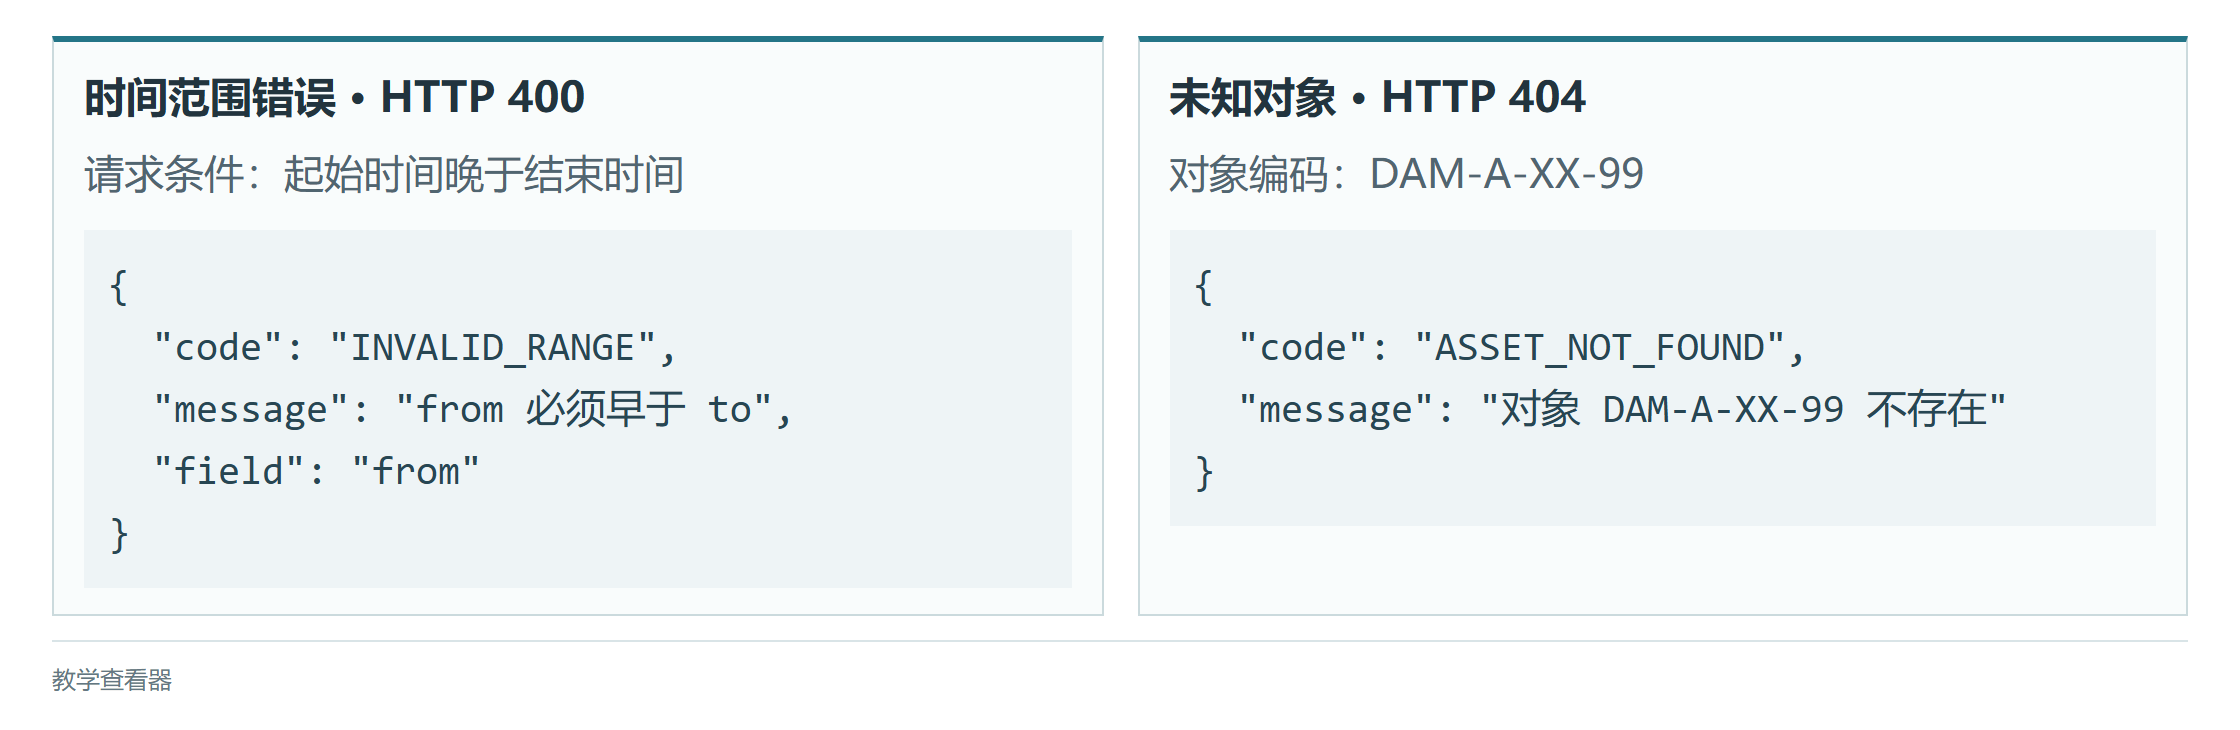
\includegraphics[width=16cm]{images/runtime/http-responses.png}
\caption{400与404错误体的实际响应（教学查看器，配套教学接口）}
\label{fig:ch05-error-results}
\end{figure}

\subsection{用第4章的页面和故障表验证接口}

写好的接口要对照契约检查，而且不止检查一次。现在这个程序只有固定数据，没有数据库，也没有登录，能检查的是表\ref{tab:ch05-first-verify}的四行：固定数据、204、404 和 400 各一例。5.4节接上数据库以后，用同样的请求再查一遍，这时对象和观测来自数据库。5.6节补上认证以后，后端才具备教学接口的全部行为，可以把第4章的 S2 页面接过来，重做表\ref{tab:ch04-stage-acceptance}的界面验收。教学接口靠\texttt{teach=}参数人为制造故障（表\ref{tab:api-teach-faults}）；真实后端没有这个参数，要用真实的请求去触发：不带令牌、把时间范围写反、请求不存在的对象、请求还没有观测的对象。

\begin{table}[htbp]
\centering
\caption{第一个接口的契约核对单}
\label{tab:ch05-first-verify}
\begin{tabular}{p{0.34\textwidth}p{0.12\textwidth}p{0.44\textwidth}}
\toprule
请求 & 期望状态 & 期望响应体 / 页面表现 \\
\midrule
GET /api/assets/DAM-A-PZ-07/readings/latest & 200 & value 185.091，页面显示“案例渗压07：185.091 kPa” \\
GET /api/assets/DAM-A-WL-01/readings/latest & 204 & 空体；页面显示“暂无观测”而不是报错 \\
GET /api/assets/DAM-A-XX-99/readings/latest & 404 & \texttt{\{code:"ASSET\_NOT\_FOUND"\}}；页面显示“对象不存在，请返回列表” \\
GET …/readings?from=2026-07-02…\&to=2026-07-01… & 400 & \texttt{\{code:"INVALID\_RANGE", field:"from"\}} \\
\bottomrule
\end{tabular}
\end{table}

\paragraph{配套工程中的位置}清单\ref{lst:ch05-first-controller}与清单\ref{lst:ch05-first-params}对应配套目录\texttt{backend/src/main/java/edu/example/lesson52/}，是 S3 阶段的起点：一个类，没有数据库，没有认证。它放在独立的包\texttt{edu.example.lesson52}里，与完整工程的\texttt{edu.example.qingyuan}分开；Spring Boot 从启动类所在的包向下扫描组件，两组控制器若被同一次扫描发现，两个\texttt{/api/assets}映射冲突，应用启动即失败。表\ref{tab:ch05-first-verify}的四行不必手工逐个点，配套工程的契约核对脚本把它们连同错误体的形状写成了可执行的检查，运行方式见清单\ref{lst:ch05-contract-check-cmd}：

\begin{lstlisting}[label={lst:ch05-contract-check-cmd},language=bash,caption={对 5.2 节的程序运行契约核对脚本}]
node teaching-api/contract-check.mjs http://localhost:8080 --stage=lesson52
\end{lstlisting}

脚本逐项打印通过或失败；失败时按它报告的路径、状态码和字段去核对程序。同一个脚本把\texttt{--stage}换成\texttt{lesson54}、\texttt{full}或\texttt{teaching}，分别核对5.4节接了数据库的程序、带认证的完整后端和教学接口，每个阶段只检查该阶段已经实现的行为。

\paragraph{自测}（1）把清单\ref{lst:ch05-first-controller}中的\texttt{@RestController}换成\texttt{@Controller}，访问\texttt{/api/assets}会发生什么？为什么？（框架把返回值当视图名去找模板，得到 404 或 500；\texttt{@RestController} = \texttt{@Controller} + \texttt{@ResponseBody}。）（2）\texttt{latest}方法为什么返回\texttt{ResponseEntity}而\texttt{assets}方法直接返回\texttt{List}？（前者需要区分 200 与 204 两种状态码，后者永远 200。）（3）不看代码，说出契约里“错误体统一为\texttt{\{code, message, field?\}}”在本节由哪两个方法保证，还有哪一类错误它们接不住。

\section{Spring Boot 工程是怎样装起来的}

\paragraph{本节层次}核心：5.3.1、5.3.2、5.3.3；拓展：5.3.4。

\paragraph{进入本节所需知识}5.2节的程序已经跑通，能从请求路径找到对应的控制器方法；读过附录B P2 单元中关于\texttt{pom.xml}和依赖注入的两段。

5.2节的程序只有一个控制器类，却能监听端口、解析路径、输出 JSON，这些事是 Spring Boot 替你做的。本节回答三个问题：这些能力从哪里来（起步依赖与自动配置，5.3.1节）；数据库地址、口令这类随环境变化的值放在哪里（配置文件，5.3.2节）；控制器需要的 Repository 和服务对象由谁创建、怎样交到它手里（依赖注入，5.3.3节）。5.4节接数据库、拆分三层时，这三样都要用到。清单\ref{lst:ch05-http}是配套工程后端部分的目录，后面提到的文件都可以在里面找到。配套工程规模小，完整后端的十几个类都放在\texttt{edu.example.qingyuan}一个包里；类多起来以后，通常再按控制器、服务、数据访问分成子包。

\begin{lstlisting}[label={lst:ch05-http},language=bash,caption={配套工程后端部分的目录}]
companion/water-platform-demo/
  backend/
    pom.xml                          # 依赖与 Java 版本
    src/main/java/edu/example/
      lesson52/                      # 5.2 节：一个控制器，固定数据
      lesson54/                      # 5.4 节入口：只装配，不含业务代码
      lesson56/                      # 5.6 节：刷新令牌校验器
      qingyuan/                      # 完整后端：控制器、服务、实体、Repository、安全配置
    src/main/resources/application.yml
    src/test/java/edu/example/       # 测试，包结构与 main 相同
  db/001_init.sql                    # 建表、约束与索引
  db/002_seed.sql                    # 五个对象和几条种子观测
\end{lstlisting}

\subsection{起步依赖：程序为什么能监听端口、输出 JSON}

\texttt{Lesson52Application}的\texttt{main}方法只有一行\texttt{SpringApplication.run(...)}，没有创建服务器的代码。监听端口的是 Tomcat，把路径分派到控制器方法的是 Spring MVC，把\texttt{List}转成 JSON 的是 Jackson。这三个库都不用自己去找：\texttt{pom.xml}里声明一个\texttt{spring-boot-starter-web}，Maven 就把它们连同相互匹配的版本一起下载下来。这种“一项能力打包成一个依赖”的坐标叫\textbf{起步依赖}（starter）。清单\ref{lst:ch05-boot-dependencies}摘自配套工程的\texttt{pom.xml}，略去了安全、消息等后面几节才用到的依赖。

\begin{lstlisting}[label={lst:ch05-boot-dependencies},language=XML,breakatwhitespace=false,caption={pom.xml：导入 Spring Boot 3.2.10 的版本清单，声明起步依赖（节选）}]
  <properties>
    <java.version>17</java.version>
    <spring-boot.version>3.2.10</spring-boot.version>
  </properties>
  <dependencyManagement>
    <dependencies>
      <dependency>
        <groupId>org.springframework.boot</groupId>
        <artifactId>spring-boot-dependencies</artifactId>
        <version>${spring-boot.version}</version>
        <type>pom</type>
        <scope>import</scope>
      </dependency>
    </dependencies>
  </dependencyManagement>
  <dependencies>
    <dependency><groupId>org.springframework.boot</groupId><artifactId>spring-boot-starter-web</artifactId></dependency>
    <dependency><groupId>org.springframework.boot</groupId><artifactId>spring-boot-starter-data-jpa</artifactId></dependency>
    <dependency><groupId>org.springframework.boot</groupId><artifactId>spring-boot-starter-validation</artifactId></dependency>
    <dependency><groupId>org.postgresql</groupId><artifactId>postgresql</artifactId></dependency>
\end{lstlisting}

四个依赖都没有写版本号。版本来自\texttt{dependencyManagement}里导入的\texttt{spring-boot-}\allowbreak\texttt{dependencies}：它是一张版本清单（BOM），列出 Spring Boot 3.2.10 验证过的几百个库各自的版本，导入之后，清单里有的库一律按它取版本，Web、JPA 和 PostgreSQL 驱动之间不会因为版本不配套而出错。许多教程用的是另一种写法，在\texttt{pom.xml}开头用\texttt{<parent>}继承\texttt{spring-boot-}\allowbreak\texttt{starter-parent}。两种写法在版本管理上效果相同，因为 parent 内部也是引用这张清单；区别是 parent 还顺带配置了几个构建插件。只导入 BOM 时这些要自己写，配套\texttt{pom.xml}里编译插件的\texttt{<parameters>}\allowbreak\texttt{true</parameters>}就是一例，缺了它，\texttt{@PathVariable String assetId}这种不写参数名的绑定在运行时找不到名字，文件中的注释说明了后果。

四个起步依赖分别带来：Web（Tomcat、Spring MVC、Jackson）、数据访问（JPA 与连接池，5.4节）、请求体校验（5.5节）和 PostgreSQL 的 JDBC 驱动。Spring Boot 3 建立在 Jakarta EE 之上，所以清单中的导入语句以\texttt{jakarta.persistence}、\texttt{jakarta.servlet}开头；网上以\texttt{javax.}开头的旧示例要改包名才能编译。

库下载下来只是躺在类路径上，谁来创建 Tomcat、注册 JSON 转换器？这一步叫\textbf{自动配置}。Spring Boot 启动时检查一批条件：类路径上有 Tomcat 和 Spring MVC 的类，就创建内嵌服务器和请求分派器；有 Jackson，就注册 JSON 转换器；有 JPA 而且配置了数据库地址，就创建连接池。每一条都附带“你没有自己定义同类对象”这个前提，你定义了，默认的那份就让位。所以自动配置是一组带条件的默认值，条件和结果都查得到。

\paragraph{运行与观察}在\texttt{backend}目录执行\texttt{mvn dependency:tree}，在输出里找到\texttt{spring-boot-starter-web}一行，它下面挂着\texttt{tomcat-embed-core}、\texttt{spring-webmvc}和\texttt{jackson-databind}，版本号都不是你写的。再给5.2节的启动命令追加参数\texttt{-Dspring-boot.run.arguments=--debug}，启动日志里多出一份\texttt{CONDITIONS EVALUATION REPORT}：\texttt{Positive matches}一栏能找到\texttt{DispatcherServletAutoConfiguration}和\texttt{JacksonAutoConfiguration}，每一项后面写着它成立的条件；\texttt{Negative matches}一栏列出没有生效的配置和原因。以后遇到“某个功能为什么没起作用”，先读这份报告，再决定是补依赖还是改配置。

\subsection{连接配置：随环境变化的值放在哪里}

数据库地址在你的笔记本上是\texttt{localhost:5432}，在 Docker Compose 里是\texttt{postgres:5432}，到了部署环境又是另一个地址；口令各处也不同。这类值如果写在 Java 代码里，每换一个环境就要改代码、重新编译。Spring Boot 的做法是把它们集中写在\texttt{src/main/resources/application.yml}中，程序启动时读取。YAML 用缩进表示层级，\texttt{spring.datasource.url}这个配置项写出来就是\texttt{spring:}下面缩进一层的\texttt{datasource:}、再缩进一层的\texttt{url:}。

配置值可以写成占位符。配套工程里数据库地址的写法是\texttt{\$\{DB\_URL:}\allowbreak\texttt{jdbc:postgresql://}\allowbreak\texttt{localhost:5432/qingyuan\}}，读作：环境变量\texttt{DB\_URL}有值就用它，没有就用冒号后面的默认值。同一份文件因此不加修改就能用在本机和容器里，差别只在启动前设了哪些环境变量。5.4.1节接数据库时用到的就是这一段（清单\ref{lst:ch05-db-config}），这里先弄清它的读法。

口令为什么不写进仓库？仓库会被克隆、分享、公开，提交历史里出现过一次的口令，删掉文件也抹不掉。配套工程的\texttt{application.yml}给\texttt{DB\_PASSWORD}留了默认值\texttt{teaching-only}，是为了让读者克隆下来就能运行，它对应的数据库只监听本机的 127.0.0.1。部署到多人可以访问的环境时，配置文件里只保留\texttt{\$\{DB\_PASSWORD\}}、不给默认值，口令由运维通过环境变量或密钥文件提供；没提供时应用启动失败并指出缺少哪个变量，比带着一个人人知道的口令运行要好。5.6节的 JWT 签名密钥按同样的办法处理。

环境之间差别较多时，可以按 Profile 拆文件：公共部分留在\texttt{application.yml}，某个环境特有的部分放进\texttt{application-test.yml}这样的文件，启动时用环境变量\texttt{SPRING\_PROFILES\_ACTIVE=test}选择。配套工程的差别只有几个地址和口令，用占位符就够了，没有拆分。预警阈值、特征水位这类业务参数不属于环境差异，它们以表\ref{tab:case-parameters}为准，不能在各环境的配置文件里各写一份。

\paragraph{运行与观察}环境变量不只能填占位符，还能直接覆盖配置项，规则是把配置项名字里的点换成下划线、字母大写：\texttt{server.port}对应\texttt{SERVER\_PORT}。先设置\texttt{SERVER\_PORT=8081}（PowerShell 写作\texttt{\$env:SERVER\_PORT=8081}，macOS/Linux 写作\texttt{export SERVER\_PORT=8081}），再启动5.2节的程序，日志变成\texttt{Tomcat started on port 8081}，浏览器要改用 8081 端口访问；代码和配置文件都没有动。练习后关闭这个终端，或把变量清掉，免得影响后面的步骤。

\subsection{构造器注入：对象由谁创建}

5.4节的控制器要用到两个对象：查测点台账的\texttt{AssetRepository}和查观测的\texttt{ReadingService}；\texttt{ReadingService}自己又要用\texttt{ReadingRepository}。按学过的 Java 写法，控制器里应当有一行\texttt{new ReadingService(new ...)}。配套工程里却找不到这样的代码，控制器只在构造器参数里写明“我需要这两个对象”，见清单\ref{lst:ch05-di-constructor}。

\begin{lstlisting}[label={lst:ch05-di-constructor},language=Java,caption={用构造器参数声明“我需要什么”（摘自配套工程的两个类）}]
// ReadingService.java
@Service
public class ReadingService {
    private final ReadingRepository repository;
    public ReadingService(ReadingRepository repository) { this.repository = repository; }
    // ……
}

// AssetController.java
@RestController
@RequestMapping("/api/assets")
public class AssetController {
    private final AssetRepository assets;
    private final ReadingService readings;

    public AssetController(AssetRepository assets, ReadingService readings) {
        this.assets = assets; this.readings = readings;
    }
    // ……
}
\end{lstlisting}

\paragraph{谁 new 的}是 Spring 的容器。应用启动时，它从启动类所在的包向下扫描，找出带\texttt{@RestController}、\texttt{@Service}、\texttt{@Component}这类注解的类和 Repository 接口，为每个类创建一个对象。由容器创建和保管的对象叫 \textbf{Bean}。创建某个类之前，容器先看它的构造器需要哪些类型的参数，把那些类型的 Bean 先创建好再传进去。上面的例子里，顺序是\texttt{ReadingRepository}、\texttt{ReadingService}，然后才轮到\texttt{AssetController}。类只声明需要什么，由外部创建好再交给它，这种做法叫\textbf{依赖注入}；通过构造器参数来交，叫构造器注入。每种 Bean 默认只创建一个，所有请求共用，这一点的后果在5.3.4节说明。

\paragraph{为什么用构造器而不是字段}Spring 也允许在字段上写\texttt{@Autowired}，由容器在对象创建之后用反射把值填进去。本书的清单一律用构造器，理由有三条。字段可以声明成\texttt{final}，赋值一次之后不会被改动。对象只要创建出来，依赖就是齐全的，不存在“创建了但某个字段还是\texttt{null}”的中间状态。第三条最实用：不启动 Spring 也能创建这个类的对象，测试时自己调用构造器、自己传参数就行，字段注入的类离开容器则没法填那个字段。

\paragraph{测试时怎么传假的}清单\ref{lst:ch05-di-fake}测试\texttt{ReadingService.latest}在“测点还没有观测”时的行为。\texttt{mock(}\allowbreak\texttt{ReadingRepository.class)}用 Mockito（测试起步依赖自带）生成一个假的 Repository：它实现了接口的全部方法，默认什么都不做，\texttt{when(...).thenReturn(...)}规定某个方法被调用时返回什么。然后像普通 Java 一样\texttt{new ReadingService(fake)}。整个测试不连数据库、不启动 Spring，几十毫秒就跑完。

\begin{lstlisting}[label={lst:ch05-di-fake},language=Java,caption={自己调用构造器，传入假的 Repository（书中示例）}]
import static org.assertj.core.api.Assertions.assertThat;
import static org.mockito.Mockito.mock;
import static org.mockito.Mockito.when;

class ReadingServiceTest {
    @Test
    void latestIsEmptyWhenAssetHasNoReading() {
        ReadingRepository fake = mock(ReadingRepository.class);
        when(fake.findFirstByIdAssetIdOrderByIdOccurredAtDescIdVersionDesc("DAM-A-D-01"))
                .thenReturn(Optional.empty());

        ReadingService service = new ReadingService(fake);   // 没有 Spring，就是普通的 new

        assertThat(service.latest("DAM-A-D-01")).isEmpty();
    }
}
\end{lstlisting}

\paragraph{一个会遇到的失败}5.4.2节的程序跑通以后，把\texttt{ReadingService}类上的\texttt{@Service}注释掉，用完整工程的入口\texttt{WaterPlatformApplication}启动。应用启动失败，日志末尾的\texttt{APPLICATION FAILED TO START}下面有一句\texttt{required a bean of type 'edu.example.qingyuan.ReadingService' that could not be found}，前半句指出是哪个类的构造器的第几个参数。原因是去掉注解以后，扫描时不再把这个类当作 Bean，需要它的类就创建不出来。恢复注解后重新启动。5.4节的\texttt{Lesson54Application}用\texttt{@Import}直接点名装入\texttt{ReadingService}，不依赖扫描，所以这个试验要用完整工程的入口来做。

\paragraph{自测}（1）\texttt{AssetController}的构造器有两个参数，容器按什么顺序创建这三个对象？依据是什么？（2）清单\ref{lst:ch05-di-fake}里的\texttt{service}是 Bean 吗？（不是，它是测试代码自己创建的普通对象，容器不知道它。）（3）把\texttt{ReadingService}改成字段注入，清单\ref{lst:ch05-di-fake}的测试还能这样写吗？

\subsection{框架在背后做的另外几件事}

这一小节是选读，列出容器的三个行为。它们平时看不见，出问题时需要知道从哪里找原因。

\paragraph{Bean 是单例，字段不能存请求数据}\texttt{ReadingService}在整个应用里只有一个对象，Tomcat 的几十个工作线程同时调用它。如果在服务类里加一个字段\texttt{private String currentAssetId}，在方法开头赋值、后面读取，两个并发请求就会互相覆盖：值班员甲查 PZ-07，拿到的可能是值班员乙刚查的 WL-01 的数据。这种错误单人测试时发现不了。Bean 的字段只放构造器注入进来的、同样无状态的协作对象；每次请求的数据通过方法参数和局部变量传递。

\paragraph{注解靠代理生效}\texttt{@Transactional}、\texttt{@PreAuthorize}、\texttt{@Cacheable}这类注解本身不执行任何代码。容器发现某个 Bean 上有它们，注入给别人的就不是原对象，而是一个包了一层的\textbf{代理}：外部调用先到代理，代理开启事务或检查权限，再转给原对象。由此得到两条规则：只有经过容器注入的对象才带这些行为，清单\ref{lst:ch05-di-fake}里自己\texttt{new}出来的\texttt{service}没有事务；同一个类内部用\texttt{this.方法()}互相调用不经过代理，被调用方法上的注解不起作用。第二条是事务最常见的失效原因，5.4.5节给出例子。

\paragraph{需要关闭的资源}线程池、外部连接这类对象要在应用停止时关闭。用\texttt{@Bean}方法创建的对象，Spring 在关闭时会寻找它的\texttt{close()}或\texttt{shutdown()}方法并调用；也可以用\texttt{@Bean(destroyMethod = "shutdown")}明确指定，指定的方法必须真实存在。Java 17 的\texttt{ExecutorService}只有\texttt{shutdown()}，\texttt{close()}是 Java 19 才加上的，写成\texttt{destroyMethod = "close"}会在启动时报找不到销毁方法。自己写的组件可以在一个方法上标\texttt{@PreDestroy}完成清理。数据库连接池由自动配置创建和关闭，不用操心。

\section{Jakarta Persistence与事务管理}

\paragraph{本节层次}核心：5.4.1、5.4.2、5.4.4、5.4.5、5.4.6；指导实践：5.4.3、5.4.7；拓展：5.4.8、5.4.9、5.4.10、5.4.11。标为拓展的四个小节是选读，前面七个小节不依赖它们。

\paragraph{进入本节所需知识}5.3节的连接配置与构造器注入；附录B P3 单元，能解释表、主键、外键、参数化查询和事务。


\subsection{把固定数据换成数据库查询}\label{sec:ch05-db-step}

\paragraph{业务问题}5.2节的四个测点写在 Java 代码里。工程上新装一支渗压计，就得改代码、重新编译、重新部署；历史观测的查询也一直返回空列表。测点台账和观测本来就存放在数据库的\texttt{asset}和\texttt{reading}两张表里（教学用到的列见附录B P3 单元的表\ref{tab:prep-p3-tables}，完整表结构见配套工程的\texttt{db/001\_init.sql}），现在让接口去读这两张表。接口的路径、字段和状态码一律不变，第4章的页面不应察觉数据来源换过。

要补三样东西：一个与\texttt{asset}表对应的 Java 类（实体），一个负责查询的接口（Repository），以及数据库的连接配置。

\paragraph{实体：一行记录对应一个对象}清单\ref{lst:ch05-db-entity}是配套工程的\texttt{AssetEntity.java}。\texttt{@Entity}声明这个类的对象与数据库表的行对应，\texttt{@Table}指出表名，\texttt{@Id}标出主键字段。字段名\texttt{assetId}与列名\texttt{asset\_id}的对应不用逐个声明：Spring Boot 默认把驼峰写法的字段名转换成下划线写法的列名。无参构造器留给框架，它从数据库读出一行后，先用无参构造器创建对象再填入各字段；业务代码使用带参数的构造器。实体只有读取方法、没有\texttt{set}方法，业务代码拿到对象后无法随手改动它的字段。表里的\texttt{geometry}、\texttt{elevation\_m}等列在实体中没有对应字段，这是允许的：实体只需声明本程序用到的列，空间位置到第6章才用。

\begin{lstlisting}[label={lst:ch05-db-entity},language=Java,caption={AssetEntity：与 asset 表对应的实体}]
package edu.example.qingyuan;

import jakarta.persistence.Entity;
import jakarta.persistence.Id;
import jakarta.persistence.Table;

@Entity
@Table(name = "asset")
public class AssetEntity {
    @Id private String assetId;
    private String assetType;
    private String displayName;
    private String unit;
    private boolean active = true;
    protected AssetEntity() {}
    public AssetEntity(String assetId, String assetType, String displayName, String unit) {
        this.assetId = assetId; this.assetType = assetType; this.displayName = displayName; this.unit = unit;
    }
    public String getAssetId() { return assetId; }
    public String getAssetType() { return assetType; }
    public String getDisplayName() { return displayName; }
    public String getUnit() { return unit; }
    public boolean isActive() { return active; }
}
\end{lstlisting}

\paragraph{Repository：只声明方法，不写实现}清单\ref{lst:ch05-db-repository}是一个接口，全工程找不到它的实现类。应用启动时，Spring Data 读取接口中的方法名，按“\texttt{findBy} + 条件 + \texttt{OrderBy} + 排序字段”的规则生成查询：\texttt{findByActiveTrue}\allowbreak\texttt{OrderByAssetId}被翻译成一条查询语句，大意是\texttt{select ... from asset}\allowbreak\texttt{ where active = true}\allowbreak\texttt{ order by asset\_id}。继承\texttt{JpaRepository<AssetEntity, String>}还带来一批现成的方法，两个类型参数分别是实体类型和主键类型，5.4.2节要用的\texttt{existsById}就在其中。方法名里的\texttt{Active}、\texttt{AssetId}必须与实体字段名对应；拼错了，编译照样通过，错误要到应用启动时才暴露，本小节末尾的故障练习会让你读一次这条错误。

\begin{lstlisting}[label={lst:ch05-db-repository},language=Java,caption={AssetRepository：由方法名派生查询}]
package edu.example.qingyuan;

import java.util.List;
import org.springframework.data.jpa.repository.JpaRepository;

public interface AssetRepository extends JpaRepository<AssetEntity, String> {
    List<AssetEntity> findByActiveTrueOrderByAssetId();
}
\end{lstlisting}

\paragraph{控制器：只改数据来源}控制器的改动见清单\ref{lst:ch05-db-controller}，其余部分与5.2节相同。原来的\texttt{FIXED}列表删去，换成一个\texttt{AssetRepository}类型的字段。这个字段由构造器参数赋值，而全工程没有哪一行代码调用这个构造器：应用启动时，框架先创建 Repository 的实例，再把它作为参数创建控制器，这就是5.3.3节讲的构造器注入（构造器的第二个参数\texttt{ReadingService}在5.4.2节说明）。配套文件里每个接口方法上方还多一行\texttt{@PreAuthorize(...)}，那是5.6节的权限声明，启用认证之前不起作用，清单中略去。\texttt{AssetDto.from}把实体转换成接口约定的响应对象；\texttt{map(AssetDto::from)}中的\texttt{AssetDto::from}是方法引用，等价于 lambda 表达式\texttt{e -> AssetDto.from(e)}。实体不直接作为响应体返回，原因有两个。第一，表里以后可能增加只供内部使用的列（例如停用原因），它们不应自动出现在接口上。第二，接口字段一旦交给前端使用就不能随便改，而表结构还会调整。DTO（数据传输对象）就是隔在两者之间的一层。

\begin{lstlisting}[label={lst:ch05-db-controller},language=Java,caption={AssetController 的改动：注入 Repository，用查询结果替换固定列表}]
// —— AssetController.java 中发生变化的部分 ——
    public record AssetDto(String assetId, String displayName, String assetType, String unit) {
        static AssetDto from(AssetEntity e) {
            return new AssetDto(e.getAssetId(), e.getDisplayName(), e.getAssetType(), e.getUnit());
        }
    }

    private final AssetRepository assets;
    private final ReadingService readings;

    public AssetController(AssetRepository assets, ReadingService readings) {
        this.assets = assets; this.readings = readings;
    }
    @GetMapping
    public List<AssetDto> assets() {
        return assets.findByActiveTrueOrderByAssetId().stream().map(AssetDto::from).toList();
    }
\end{lstlisting}

\paragraph{连接配置}数据库在哪里、用什么账号连接，写在\texttt{src/main/resources/application.yml}中（清单\ref{lst:ch05-db-config}）。\texttt{\$\{DB\_URL:jdbc:postgresql://...\}}的含义是：有环境变量\texttt{DB\_URL}就用它，没有就用冒号后面的默认值，同一份配置文件因此可以不加修改地用于本机和容器。DDL 指建表、改表这类语句；\texttt{ddl-auto: validate}表示应用启动时只核对实体与表结构、不做改动，对不上就拒绝启动；表由\texttt{db/001\_init.sql}创建，应用本身不建表也不改表。

\begin{lstlisting}[label={lst:ch05-db-config},language=YAML,caption={application.yml 中的数据源配置}]
spring:
  datasource:
    url: ${DB_URL:jdbc:postgresql://localhost:5432/qingyuan}
    username: ${DB_USER:qingyuan_app}
    password: ${DB_PASSWORD:teaching-only}
  jpa:
    open-in-view: false
    hibernate.ddl-auto: validate
\end{lstlisting}

\paragraph{观测表的实体}\texttt{reading}表的主键由三列组成：哪个对象、什么时刻、第几个版本。同一对象、同一时刻、同一版本只能有一条记录；人工订正不覆盖原值，而是追加一条版本号加1的记录，“当时采到的是什么、后来改成了什么”都查得到。清单\ref{lst:ch05-db-reading-entity}用\texttt{@EmbeddedId}把这三列组合成一个主键对象\texttt{ReadingId}；\texttt{@Embeddable}表示\texttt{ReadingId}自己不对应一张表，它的三个字段嵌入\texttt{reading}表的三列；JPA 规范要求复合主键类实现\texttt{Serializable}。\texttt{value}的类型是\texttt{BigDecimal}而不是\texttt{double}：表中这一列是十进制的\texttt{numeric}，实体写成\texttt{Double}会在启动核对时被拒绝；二进制浮点数也无法精确表示 0.1、185.091 这样的十进制小数，误差会在累加和比较时显现（\texttt{0.1 + 0.2 == 0.3}为假），日降雨量累计、与阈值比较都属于这类运算。缺测时\texttt{value}为\texttt{null}，与 0 是两回事。

\begin{lstlisting}[label={lst:ch05-db-reading-entity},language=Java,caption={ReadingEntity：复合主键与带单位的观测值（节选）}]
@Entity
@Table(name = "reading")
public class ReadingEntity {
    @EmbeddedId private ReadingId id;
    // 幂等键：一次上报一个 eventId，重复收到时靠它识别
    @Column(name = "event_id", nullable = false) private String eventId;
    // 表中是 numeric 列，对应 BigDecimal；缺测时为 null，不是 0
    @Column(name = "value") private BigDecimal value;
    @Column(nullable = false) private String unit;
    @Column(nullable = false) private String quality;
    @Column(nullable = false) private String source;
    // ……构造器与访问方法略，见配套文件

    @Embeddable
    public record ReadingId(@Column(name = "asset_id") String assetId,
                            @Column(name = "occurred_at") OffsetDateTime occurredAt,
                            int version) implements java.io.Serializable {}
}
\end{lstlisting}

清单\ref{lst:ch05-db-reading-repository}是观测的 Repository。按时间窗查询不适合用方法名表达，改用\texttt{@Query}写出查询语句。这种语句叫 JPQL，写法与 SQL 相近，但\texttt{from}后面是实体类名，条件里用的是字段名（\texttt{r.id.occurredAt}）而不是列名。语句两端的三个双引号是 Java 的多行字符串；\texttt{:assetId}是命名参数，运行时由标了\texttt{@Param("assetId")}的方法参数填入，值与语句分开传递，就是附录B P3 单元讲的参数化查询。时间窗取左闭右开$[\mathit{from}, \mathit{to})$：查询“7月1日”和“7月2日”两天时，7月2日零点整的那条观测只出现在后一天的结果里，两天的结果拼接起来既不重复也不遗漏，统计日降雨量、日平均渗压时不会把边界上的观测算两次。取最新观测仍由方法名派生。方法名中的\texttt{IdAssetId}要读成\texttt{id.assetId}，即先进入主键对象\texttt{id}，再取其中的\texttt{assetId}；\texttt{First}表示只取一条。排序先按时间倒序，同一时刻再按版本号倒序，取到的是订正后的值。

\begin{lstlisting}[label={lst:ch05-db-reading-repository},language=Java,caption={ReadingRepository：时间窗查询与最新一条}]
package edu.example.qingyuan;

import java.time.OffsetDateTime;
import java.util.List;
import java.util.Optional;
import org.springframework.data.jpa.repository.JpaRepository;
import org.springframework.data.jpa.repository.Query;
import org.springframework.data.repository.query.Param;

public interface ReadingRepository extends JpaRepository<ReadingEntity, ReadingEntity.ReadingId> {
    /** [from, to)：相邻查询窗口的共同边界只出现在后一个窗口。 */
    @Query("""
            select r from ReadingEntity r where r.id.assetId = :assetId
            and r.id.occurredAt >= :from and r.id.occurredAt < :to
            order by r.id.occurredAt, r.id.version
            """)
    List<ReadingEntity> findInWindow(@Param("assetId") String assetId,
            @Param("from") OffsetDateTime from, @Param("to") OffsetDateTime to);
    boolean existsByEventId(String eventId);

    /** 契约 GET /api/assets/{id}/readings/latest：同一时刻可能有多个版本，取版本号最大的那条。 */
    Optional<ReadingEntity> findFirstByIdAssetIdOrderByIdOccurredAtDescIdVersionDesc(String assetId);
}
\end{lstlisting}

\paragraph{运行与观察}这一步的可运行入口是配套工程的\texttt{edu.example.lesson54.Lesson54Application}。它没有自己的业务代码，只把上面几个类和5.4.2节的服务类装配起来，不启用认证，也不连接消息队列。配套工程只保留拆成三层之后的版本，5.4.1节和5.4.2节因此共用这一个入口；“全都写在控制器里”的中间状态只出现在书中的讲解里。先停掉5.2节的程序，按\texttt{STAGES.md}“S3 中点”的命令用 Docker 启动 PostgreSQL（初始化脚本自动建表并写入五个对象和几条观测），再启动这个入口。表\ref{tab:ch05-db-run}是应当看到的结果。

\begin{table}[htbp]
\centering
\caption{接入数据库后的预期运行记录}
\label{tab:ch05-db-run}
\begin{tabular}{p{0.44\textwidth}p{0.08\textwidth}p{0.40\textwidth}}
\toprule
操作 & 状态码 & 观察 \\
\midrule
浏览器打开 /api/assets & 200 & 五个对象，按编码排序；比5.2节多出\texttt{DAM-A-PZ-08}，它来自数据库而不是代码 \\
在数据库中执行\texttt{UPDATE asset SET active = false WHERE asset\_id = 'DAM-A-RF-01'}后刷新（执行方法和恢复命令见\texttt{STAGES.md}） & 200 & 只剩四个对象；程序没有重启，代码没有改动。练习后把\texttt{active}改回\texttt{true} \\
/api/assets/DAM-A-D-01/readings/latest & 204 & 位移计已登记、尚无观测 \\
/api/assets/DAM-A-PZ-07/readings，时间窗取宽，如\texttt{from=2026-01-01T00:00:00Z}、\texttt{to=2030-01-01T00:00:00Z} & 200 & 五条种子观测，其中一条\texttt{value}为\texttt{null}、\texttt{quality}为\texttt{missing}；时间以 UTC（末尾带 Z）给出，与带\texttt{+08:00}的写法指同一时刻 \\
运行契约核对脚本，\texttt{--stage=lesson54} & — & 全部通过；状态码、字段名和错误体与5.2节一致 \\
\bottomrule
\end{tabular}
\end{table}

\paragraph{一个会遇到的失败}把清单\ref{lst:ch05-db-repository}的方法名改成\texttt{findByActiveTrueOrderByAssetCode}再启动。编译通过，应用却启动失败，日志末尾有一行\texttt{PropertyReferenceException: No property 'assetCode' found for type 'AssetEntity'}。原因是 Spring Data 在启动时解析方法名，\texttt{AssetEntity}没有名为\texttt{assetCode}的字段。改回\texttt{AssetId}后重新启动，再访问\texttt{/api/assets}确认恢复。另一个常见失败是数据库没有启动或口令不符，日志中出现\texttt{Connection refused}或\texttt{password authentication failed}，应用同样拒绝启动。这类错误都要从启动日志的最后一个\texttt{Caused by}读起，它指向最初的原因。

\paragraph{自测}（1）\texttt{AssetRepository}没有实现类，\texttt{assets.findByActiveTrueOrderByAssetId()}调用的代码从哪里来？（Spring Data 在启动时按方法名生成实现。）（2）把\texttt{ddl-auto}从\texttt{validate}改成\texttt{update}，应用会按实体自动改表。监测平台为什么不这样做？（表结构由迁移脚本统一管理并经过评审；让程序自动改表，观测表的约束和索引可能在无人知晓时被改动。）（3）时间窗为什么取左闭右开而不是两端都闭？

\subsection{从一个类到三层}\label{sec:ch05-layer-step}

\paragraph{业务问题}接入数据库以后，“取最新观测”这个接口要回答的问题变多了：这个对象存在吗？存在的话，最新的一条是哪条？同一时刻有订正版本时取哪个？一条也没有时怎么应答？这些判断如果都写在控制器方法里，控制器既要处理 HTTP，又要懂业务规则，还要知道怎样查库。5.7节的消息消费者收到新观测时，也需要“按对象和时间查观测”“写入前检查是否重复”这些能力，而它根本不经过 HTTP，控制器里的代码它用不上。解决办法是把代码按职责分到三层，每层只回答一类问题，如图\ref{fig:ch05-request-chain}所示。

\paragraph{服务层}清单\ref{lst:ch05-rest-layer}是配套工程的\texttt{ReadingService}。\texttt{@Service}把它登记为由框架创建和注入的组件。它对外提供两个查询方法，调用者不需要知道底下是哪一条 SQL。\texttt{latest}返回\texttt{Optional}：有观测就装着那条观测，没有就是空的。“没有观测”在这里是一种正常结果，不是异常；它对应 HTTP 的哪个状态码，服务层不关心，也不应该关心，因为调用它的不一定是 HTTP 请求。方法上的\texttt{@Transactional(readOnly = true)}与事务有关。事务是一组要么全部生效、要么全部不生效的数据库操作（附录B P3 单元），服务层的方法通常以它为单位执行。这两个方法只查不改，谈不上“全部不生效”；加上这个注解，是让方法里的查询共用同一个数据库连接，并向框架说明这里只读，Hibernate 因此不必为查出来的对象保留用于比对改动的副本。写入方法上的事务在5.4.4节和5.4.5节展开。

\begin{lstlisting}[label={lst:ch05-rest-layer},language=Java,caption={ReadingService：服务层的两个查询方法}]
@Service
public class ReadingService {
    private final ReadingRepository repository;
    public ReadingService(ReadingRepository repository) { this.repository = repository; }

    @Transactional(readOnly = true)
    public List<ReadingEntity> find(String assetId, OffsetDateTime from, OffsetDateTime to) {
        return repository.findInWindow(assetId, from, to);
    }

    /** 最新一条观测；对象存在但尚无观测时返回空，由控制层按契约转成 204。 */
    @Transactional(readOnly = true)
    public Optional<ReadingEntity> latest(String assetId) {
        return repository.findFirstByIdAssetIdOrderByIdOccurredAtDescIdVersionDesc(assetId);
    }
    // ……幂等写入方法 accept(...) 见配套文件
}
\end{lstlisting}

\paragraph{控制器：协议转换，加一次存在性查询}清单\ref{lst:ch05-layer-controller}是拆分之后控制器里的\texttt{latest}方法。它做三件事：用\texttt{existsById}确认对象存在，不存在就抛出异常，由统一的异常处理（5.5.2节）转换成 404 和契约错误体；调用服务层取最新观测；把服务层返回的\texttt{Optional}翻译成 HTTP 应答，有值时转换成\texttt{ReadingDto}并应答 200，空值时应答 204。5.1节说的“204 与 404 要分开”，落到代码上就是这两个分支。

\begin{lstlisting}[label={lst:ch05-layer-controller},language=Java,caption={AssetController.latest：对象不存在 404，尚无观测 204}]
    @GetMapping("/{assetId}/readings/latest")
    public ResponseEntity<ReadingDto> latest(@PathVariable String assetId) {
        if (!assets.existsById(assetId)) {
            throw new AssetNotFoundException(assetId);
        }
        return readings.latest(assetId)
                .map(ReadingDto::from)
                .map(ResponseEntity::ok)
                .orElseGet(() -> ResponseEntity.noContent().build());
    }
\end{lstlisting}

\paragraph{哪些查询可以留在控制器里}第一件事里，控制器直接调用了\texttt{AssetRepository}，没有经过服务层。配套工程是这样划界的：控制器负责 HTTP 协议转换，也可以直接用 Repository 做“这个编码存在吗”这种不含业务规则的单次查询；含有规则的查询，以及会被别的入口复用的查询与写入，放在服务层。“取最新观测”含有规则（同一时刻取订正后的版本），消息消费者写入观测时也要用到服务层的方法，所以它们在\texttt{ReadingService}里。“编码是否登记过”只是按主键查一次，没有规则可言，目前也只有 HTTP 入口关心它（消费者写入时由外键约束把关）；为它单设一个只转发一行的服务方法，得不到什么。这条界线会随需求移动。以后“存在”如果要附带条件，例如已停用的测点对值班员视为不存在，或者不同角色能看到的测点范围不同，它就成了业务规则，应当挪进服务层，让所有入口得到同一个答案。控制器里针对同一件事出现第二次查询，或者开始读取查出来的对象的字段做判断（例如\texttt{asset.isActive()}），也是该挪的信号。

\paragraph{依赖方向}依赖只朝一个方向：控制器依赖服务，也可以像上面那样直接依赖 Repository；服务依赖 Repository 接口；Repository 的实现依赖数据库。反过来不成立，Repository 不知道有服务，服务不知道有控制器。\texttt{ReadingService}的代码里没有出现任何 HTTP 或 JSON 的类型，单元测试可以直接创建它，传入一个假的 Repository 来检验规则，5.3.3节的清单\ref{lst:ch05-di-fake}就是这样做的。图\ref{fig:ch05-rest-contract}标出一次请求可能在哪个边界上失败，以及各自对应的状态码：格式问题在控制器被拒绝（400），对象不存在或状态冲突由业务判断得出（404、409）。测试接口时，除了断言状态码，还应核对响应字段，并确认失败的请求没有留下写了一半的数据。

\begin{figure}[htbp]
\centering
\begin{tikzpicture}[>=Stealth,thick,
  boundary/.style={draw=Primary,rounded corners=2pt,text width=2.7cm,minimum height=.85cm,align=center,fill=PrimaryLight,text=PrimaryDark,font=\scriptsize},
  error/.style={boundary,draw=Accent,fill=white}]
  \node[boundary] (http) at (0,0) {HTTP请求\\方法、路径、JSON};
  \node[boundary] (validate) at (3.7,0) {Controller\\格式校验};
  \node[boundary] (usecase) at (7.4,0) {Application Service\\用例、规则与事务};
  \node[boundary] (dto) at (11.1,0) {响应映射与DTO\\稳定的外部字段};
  \node[boundary] (repo) at (7.4,-1.8) {Repository\\查询与持久化};
  \node[error] (bad) at (3.7,-1.8) {400\\输入错误};
  \node[error] (domain) at (11.1,-1.8) {404/409\\对象不存在/状态冲突};
  \draw[->,Primary] (http)--(validate);
  \draw[->,Primary] (validate)--(usecase);
  \draw[->,Primary] (usecase)--(dto);
  \draw[<->,Primary] (usecase)--(repo);
  \draw[->,Accent] (validate)--(bad);
  \draw[->,Accent] (usecase.south east)--(domain.north west);
\end{tikzpicture}
\caption{REST接口的契约边界与失败返回}
\label{fig:ch05-rest-contract}
\end{figure}

\paragraph{运行与观察}仍然使用\texttt{Lesson54Application}。从5.2节的一个类，到接上数据库，再到拆成三层，程序内部变了三次，\texttt{--stage=lesson52}与\texttt{--stage=lesson54}核对的却是同一份契约，状态码、字段名和错误体都没有变。重构指的就是这种改动：内部结构变了，对外的行为不变；判断重构有没有改坏东西，靠的是这类可以重复执行的检查。再做一个反向试验：把清单\ref{lst:ch05-layer-controller}中\texttt{existsById}的判断删掉，重新启动后请求\texttt{/api/assets/DAM-A-XX-99/readings/latest}。应答从 404 变成了 204，一个不存在的对象被报告成“暂无观测”，契约核对脚本在“返回 404”这一项上报告失败。恢复这段判断后重新核对。

\paragraph{自测}（1）\texttt{ReadingService.latest}为什么返回\texttt{Optional}，而不是在没有观测时抛出异常？（没有观测是正常结果；是否算错误、用哪个状态码表达，由调用方决定。）（2）消息消费者收到一条观测后需要写入数据库，它应该调用控制器、服务还是 Repository？为什么？（3）如果让\texttt{ReadingService}直接返回\texttt{ResponseEntity}，哪一条依赖方向被破坏了？（4）\texttt{latest}方法里的\texttt{existsById}直接调用了 Repository。举一个需求变化的例子，说明它什么时候应当挪进服务层。

\subsection{分页与稳定排序}

\paragraph{业务问题}\texttt{findInWindow}把时间窗里的观测全部取回。渗压计按5分钟一条计，一天288条，页面画一条日曲线没有问题；分析员把时间窗拉到一年，就是十万多条，全部装进内存、转成 JSON、经网络送到浏览器，数据库连接、服务器内存和页面都吃不消。列表类接口要守两条规矩：一次返回多少条有上限；翻页时既不重复也不漏掉。

时间窗是第一道限制，它是契约里的必填参数。第二道限制是在时间窗内分页。Spring Data 用\texttt{Pageable}表示“第几页、每页几条、按什么排序”，查询方法的返回类型写成\texttt{Page}，框架会多发一条\texttt{count}查询，把总条数和总页数一并带回。清单\ref{lst:ch05-pageable-repository}在5.4.1节的 Repository 和5.4.2节的服务上各加一个方法。

\begin{lstlisting}[label={lst:ch05-pageable-repository},language=Java,caption={时间窗内的分页查询：页大小设上限，排序写明（书中示例）}]
// —— ReadingRepository 中新增 ——
    @Query("""
            select r from ReadingEntity r where r.id.assetId = :assetId
            and r.id.occurredAt >= :from and r.id.occurredAt < :to
            """)
    Page<ReadingEntity> findPageInWindow(@Param("assetId") String assetId,
            @Param("from") OffsetDateTime from, @Param("to") OffsetDateTime to,
            Pageable pageable);

// —— ReadingService 中新增 ——
    private static final int MAX_PAGE_SIZE = 500;

    @Transactional(readOnly = true)
    public Page<ReadingEntity> findPage(String assetId, OffsetDateTime from,
                                        OffsetDateTime to, int page, int size) {
        int bounded = Math.min(Math.max(size, 1), MAX_PAGE_SIZE);
        Pageable request = PageRequest.of(page, bounded,
                Sort.by("id.occurredAt", "id.version").ascending());
        return repository.findPageInWindow(assetId, from, to, request);
    }
\end{lstlisting}

\paragraph{页大小由服务端封顶}\texttt{size}来自请求参数，调用方写\texttt{size=1000000}，分页就形同虚设，所以服务层把它夹在 1 和 500 之间。页码从 0 开始是 Spring Data 的约定，接口文档里要写明。

\paragraph{排序必须能分出先后}数据库不保证没有\texttt{ORDER BY}的查询按什么顺序返回；排序键有并列时，并列的几行谁先谁后也不确定，两次查询可能不同。假如只按\texttt{occurredAt}排序，而某一时刻恰好有原始值和订正值两个版本，它们又正好落在页的边界上，那么第一页末尾和第二页开头可能是同一行，另一行则哪一页都不出现。办法是让排序键的组合唯一。对一个测点来说，\texttt{(occurredAt, version)}是主键去掉对象编码后剩下的部分，不会并列，清单中的\texttt{Sort}就按这两项写。

页码分页每翻一页都要数据库从头数到偏移位置，页码越大越慢，\texttt{count}查询在大表上也不便宜。只需要“继续往后加载”的场景可以改用游标分页：记住上一页最后一行的排序键，下一页从它后面取，见附录C的“分页、游标与查询预算”。导出全年数据这类耗时操作不放在一次请求里等：接口先应答\texttt{202 Accepted}并给出任务地址，由客户端轮询任务状态。

到这里已经用过两种写查询的办法：方法名派生和\texttt{@Query}。表\ref{tab:ch05-jpa-query-strategies}把它们和后面会遇到的另外三种放在一起，选择时先写出业务问题，再挑够用的那一种。

\begin{table}[htbp]
\centering
\small
\caption{JPA 查询的几种写法与适用范围}
\label{tab:ch05-jpa-query-strategies}
\begin{tabular}{p{0.18\textwidth}p{0.33\textwidth}p{0.36\textwidth}}
\toprule
写法 & 适合的问题 & 使用时注意 \\
\midrule
方法名派生 & 单表、条件简单：取最新一条、判断是否存在 & 方法名与字段名逐字对应，拼错要到启动时才报错（5.4.1节） \\
\texttt{@Query} & 时间窗、多条件、需要写明排序 & 参数名与\texttt{@Param}一致；时间窗统一左闭右开 \\
\texttt{Pageable/Page} & 需要总页数、能跳页的列表 & 页大小封顶；排序键唯一；留意\texttt{count}查询的开销 \\
DTO 投影 & 列表只用到少数几列 & 查询直接返回\texttt{record}，不把整个实体带出服务层 \\
原生 SQL & PostGIS 空间函数、TimescaleDB 时间桶聚合 & 参数绑定；语句与数据库版本、迁移脚本一起评审 \\
\bottomrule
\end{tabular}
\end{table}

\subsection{写入与约束：幂等写入与订正}

\paragraph{业务问题}观测不是由页面录入的。网关把仪器读数整理成事件，经消息队列送到后端，由消费者调用服务层写入数据库。网络会抖动，网关等不到确认就重发，消息队列在消费者重启后也会把没确认的消息再投一次，所以同一条观测到达两次是常态。写入方法必须做到：同一条观测无论到达几次，库里只有一行。这就是5.1节说的幂等。消息队列怎样配置是5.7节的选学内容；服务层这个写入方法不管调用者是谁都要这样写，属于主线。

事件的形状见清单\ref{lst:ch05-reading-event}，它是配套工程的\texttt{ReadingEvent.java}。\texttt{eventId}由网关在采集时生成，重发时不变，后端靠它认出重复。

\begin{lstlisting}[label={lst:ch05-reading-event},language=Java,caption={ReadingEvent：一次观测上报携带的字段}]
/** Kafka 观测事件契约，字段与第8章 8.3 节一致。 */
public record ReadingEvent(String eventId, String assetId, OffsetDateTime occurredAt,
                           int version, BigDecimal value, String unit,
                           String quality, String source) {}
\end{lstlisting}

清单\ref{lst:ch05-accept}是\texttt{ReadingService}里的写入方法，也就是清单\ref{lst:ch05-rest-layer}末尾略去的那一段。

\begin{lstlisting}[label={lst:ch05-accept},language=Java,caption={ReadingService.accept：先预检，再由唯一索引把关}]
    /** 幂等写入：先按 eventId 预检，并发重投由数据库复合唯一索引兜底。 */
    @Transactional
    public void accept(ReadingEvent event) {
        if (repository.existsByEventId(event.eventId())) return;
        repository.saveAndFlush(new ReadingEntity(
                new ReadingEntity.ReadingId(event.assetId(), event.occurredAt(), event.version()),
                event.eventId(), event.value(), event.unit(), event.quality(), event.source()));
    }
\end{lstlisting}

\paragraph{两道防线}第一道是\texttt{existsByEventId}：查一下这个编号写过没有，写过就直接返回。绝大多数重复在这里被挡掉。只靠它还不够：两个线程同时处理同一事件的两份拷贝时，可能都查到“没写过”，然后都去插入。第二道防线在数据库。\texttt{db/001\_init.sql}给\texttt{reading}表建了一个唯一索引\texttt{reading\_event\_uidx}，覆盖\texttt{(occurred\_at, event\_id)}两列（建表语句见5.4.7节的清单\ref{lst:ch05-index-migration}）。两个并发的插入只有一个能成功，另一个被数据库拒绝，Spring 把这个错误包装成\texttt{DataIntegrityViolationException}抛出。先查后写的检查挡不住并发，唯一约束才是最终的裁决者；预检的作用是让常见的重复不必走到报错这一步。索引里带上\texttt{occurred\_at}，是因为\texttt{reading}是按时间分区的 TimescaleDB 超表，超表上的唯一索引必须包含分区列。

\paragraph{两处写法的原因}用\texttt{saveAndFlush}而不用\texttt{save}：\texttt{save}只是把对象交给 JPA，插入语句可能拖到事务提交时才发出；\texttt{saveAndFlush}让语句立刻执行，违反约束的异常就在这一行抛出，位置明确。异常在哪里接住也有讲究。\texttt{accept}方法内部不捕获它，因为数据库报错以后这个事务已经不能继续使用，只能回滚。配套工程在调用方\texttt{ReadingConsumer}里捕获，那里已经在事务之外：记一条“重复事件已忽略”的日志，然后正常返回，消息被确认，不会重投（见5.7.3节的清单\ref{lst:ch05-kafka-idempotency}）。

\paragraph{订正：追加一个版本}观测写入以后不修改、不删除。仪器故障、抄录错误需要更正时，追加一行：对象和时刻不变，\texttt{version}加1，\texttt{source}记为人工，\texttt{revision\_reason}写明原因，原来那一行原样保留。这是\texttt{reading}表把\texttt{version}放进主键的用意，也是契约表中\texttt{PUT /api/readings/\{id\}}一行“订正后的记录（版本 +1）”“观测不删除，只增版本”的含义：接口名义上是修改，落到库里是追加。这样做的理由来自监测业务。预警是依据当时的观测发出的，事后复盘要能回答“发预警那一刻系统看到的是什么值”；原值被覆盖，这个问题就无从回答。5.4.1节的“取最新一条”先按时间倒序、再按版本号倒序，取到的自然是订正后的值。

\paragraph{运行与观察}数据库按5.4.1节的方式启动后，种子数据里 PZ-07 有一条质量码为\texttt{suspect}的观测，事件编号\texttt{SEED-PZ07-004}。用清单\ref{lst:ch05-revise-sql}给它追加一个订正版本，执行方式与5.4.1节修改\texttt{active}的练习相同。

\begin{lstlisting}[label={lst:ch05-revise-sql},language=SQL,caption={订正一条可疑观测：复制原行，版本号加 1，写明原因}]
INSERT INTO reading(asset_id, occurred_at, version, event_id,
                    value, unit, quality, source, revision_reason)
SELECT asset_id, occurred_at, version + 1, 'REV-PZ07-004',
       119.0, unit, 'valid', 'manual', '人工复核：现场记录为 119.0'
FROM reading WHERE event_id = 'SEED-PZ07-004';
\end{lstlisting}

再用宽时间窗请求\texttt{/api/assets/DAM-A-PZ-07/readings}，结果从五条变成六条：同一个\texttt{occurredAt}下有两行，\texttt{version}为1的仍是\texttt{suspect}的 121.9，\texttt{version}为2的是\texttt{valid}的 119.0。画曲线时同一时刻取版本号最大的一行。把这条\texttt{INSERT}原样再执行一次，数据库报\texttt{duplicate key value violates unique constraint}：对象、时刻、版本三项与刚写入的那一行相同，主键不允许第二行。

\paragraph{需要知道的一个边界}\texttt{JpaRepository}的\texttt{save}和\texttt{saveAndFlush}对“主键已经有值”的对象先按主键查一次：库里没有就插入，有就把字段更新成新值。\texttt{ReadingEntity}的主键由调用方给出，所以如果送来的事件与库里某一行的对象、时刻、版本都相同，只是\texttt{eventId}不同，\texttt{accept}会更新那一行，而不是报主键冲突。正常的网关不会发出这样的事件，配套的教学代码也没有拦它。要让数据库层面彻底做到只追加，写入可以改用第8章清单\ref{lst:ch08-sql-idempotent-insert}那样的原生\texttt{INSERT ... ON CONFLICT DO NOTHING}语句，应用账号也不授予\texttt{reading}表的\texttt{UPDATE}和\texttt{DELETE}权限。

\paragraph{自测}（1）去掉\texttt{existsByEventId}这一行，程序还幂等吗？代价是什么？（仍然幂等，唯一索引会拒绝重复；但每次重复都要走一遍“插入、报错、回滚”，日志里也多出一批异常。）（2）去掉唯一索引、只留预检呢？（3）值班员发现昨天 14:00 的渗压值抄错了，应该修改原行还是追加版本？复盘时各有什么后果？

\subsection{事务基础}

\paragraph{业务问题}第8章的业务链里有一步“派单”：值班员确认预警以后创建处置工单。落到数据库是两条语句，一条把\texttt{warning}表中这条预警的状态从\texttt{acknowledged}改为\texttt{assigned}，一条向\texttt{work\_order}表插入工单。如果第一条执行完，第二条因为某个字段超长而失败，库里就留下一条“已派单”却找不到工单的预警；值班员看到它已经派出，不会再管，实际上没有人去现场。

\textbf{事务}就是用来排除这种中间状态的。它把几条语句捆成一个整体，结束方式只有两种：\textbf{提交}，全部生效；\textbf{回滚}，全部撤销，如同没有执行过。教科书用 ACID 四个字母概括事务的性质，放到派单这个例子里分别是：
\begin{itemize}
\item \textbf{原子性}（Atomicity）：改预警状态和插入工单要么都发生，要么都不发生。
\item \textbf{一致性}（Consistency）：提交时数据库的约束全部成立，例如工单的\texttt{warning\_id}必须指向存在的预警。应用层的规则（先确认才能派单）由代码在同一个事务里检查。
\item \textbf{隔离性}（Isolation）：另一个请求不会看到“状态已改、工单还没插入”的半成品。隔离有强弱几档，见5.4.9节选读。
\item \textbf{持久性}（Durability）：提交成功以后，即使服务器马上断电，重启后这两处修改都还在。
\end{itemize}

\paragraph{在 Spring 里怎样划定事务}在服务类的公开方法上加\texttt{@Transactional}。方法开始时框架开启事务，方法正常返回时提交，方法抛出运行时异常（\texttt{RuntimeException}及其子类）时回滚。清单\ref{lst:ch05-tx-dispatch}是第8章\texttt{WarningWorkflowService.dispatch}的骨架，完整代码见清单\ref{lst:ch08-service}。

\begin{lstlisting}[label={lst:ch05-tx-dispatch},language=Java,caption={一个事务里的两步：改预警状态，插入工单（骨架，完整代码见第8章）}]
    @Transactional
    public WorkOrderEntity dispatch(long warningId, String ownerRole,
                                    Instant dueAt, String action) {
        if (warnings.transit(warningId, "acknowledged", "assigned") == 0)   // 第一条语句
            throw new Conflict("ILLEGAL_TRANSITION", "必须先确认预警才能派单");
        return orders.save(new WorkOrderEntity(warningId, ownerRole, dueAt, action));  // 第二条
    }
\end{lstlisting}

事务的边界放在服务层的方法上，因为“一件业务上完整的事”正是服务方法表达的东西。放在控制器里，HTTP 的细节会和数据一致性搅在一起，消息消费者也用不上；放在 Repository 里又太细，每个 Repository 方法各开各的事务，两步之间就没有保护。有两个默认行为需要记住。一是回滚只针对运行时异常，方法声明抛出的受检异常默认不触发回滚，需要时写\texttt{@Transactional(rollbackFor = Exception.class)}。二是在方法里用\texttt{try/catch}把异常接住而不再抛出，框架就看不到异常，照常提交。5.4.2节的查询方法上写的是\texttt{@Transactional(readOnly = true)}，开启的是只读事务；它只是一个声明，拦不住方法里调用\texttt{save}，也不能代替数据库账号的权限控制。

\paragraph{最常见的坑：同类内部调用}5.3.4节说过，\texttt{@Transactional}靠代理生效，只有从外部经过代理进来的调用才会开启事务。清单\ref{lst:ch05-tx-self-call}的写法看上去有事务，运行时却没有。

\begin{lstlisting}[label={lst:ch05-tx-self-call},language=Java,caption={同类内部调用绕过代理，事务注解不起作用}]
@Service
public class WarningWorkflowService {
    // 控制器调用的是这个方法，它没有事务注解
    public WorkOrderEntity dispatchWithDefaults(long warningId) {
        return this.dispatch(warningId, "DUTY", Instant.now().plus(4, ChronoUnit.HOURS), "现场巡查");
        //     ^^^^ 对象内部的直接调用，不经过代理：dispatch 上的 @Transactional 没有机会生效
    }

    @Transactional
    public WorkOrderEntity dispatch(long warningId, String ownerRole, Instant dueAt, String action) {
        // ……两条语句
    }
}
\end{lstlisting}

没有事务时，两条语句各自立即生效，第二条失败，第一条已经撤不回来，正是开头描述的事故。改法有两种：把\texttt{@Transactional}标在外部实际调用的那个方法上；或者把\texttt{dispatch}移到另一个 Bean，通过构造器注入后调用。判断“有没有事务”要看调用是不是从别的 Bean 进来的，看方法上有没有注解并不可靠。

\paragraph{运行与观察}在\texttt{application.yml}里加一行\texttt{logging.level.}\allowbreak\texttt{org.springframework.}\allowbreak\texttt{transaction.}\allowbreak\texttt{interceptor:\ TRACE}，重新启动后请求一次最新观测。日志里出现成对的两行：\texttt{Getting transaction for}\allowbreak\texttt{ [edu.example.qingyuan.}\allowbreak\texttt{ReadingService.latest]}和\texttt{Completing transaction}\allowbreak\texttt{ for [...]}，这是代理在方法前后做的事。同类内部调用的那种写法看不到这两行。练习后删去这行配置。

\paragraph{事务里不要等外部系统}事务开着的时候占用一个数据库连接，改过的行还被锁着。在事务里调用短信网关、请求另一个 HTTP 服务，对方慢几秒，连接和锁就多占几秒；对方调用成功以后事务又回滚，短信也追不回来。通知、刷新缓存、发消息这类动作放到事务提交之后再做，5.7节讲具体做法。

\paragraph{自测}（1）\texttt{dispatch}里第二条语句失败时，第一条语句改过的预警状态最终是什么？依据 ACID 的哪一条？（2）方法里写了\texttt{try \{ orders.save(...); \} catch (Exception e) \{ log.warn(...); \}}，第二步失败后事务提交还是回滚？（3）为什么说\texttt{readOnly = true}不能当作权限控制？

\subsection{状态修改与并发冲突}

\paragraph{业务问题}观测只追加，预警和工单则要修改：预警的状态从\texttt{open}走到\texttt{acknowledged}、\texttt{assigned}、\texttt{closed}。两个值班员在各自的屏幕上看到同一条\texttt{open}的预警，几乎同时点了“确认”。按“先读出来，判断状态是 open，再写回 acknowledged”的写法，两个请求都读到\texttt{open}，都通过判断，都写入成功，两个人都以为是自己确认的，后面各自派单，现场就会收到两张工单。后写的人悄悄盖掉先写的人的结果，这类问题叫\textbf{丢失更新}。

\paragraph{主要做法：带状态条件的更新}把“我期望的旧状态”写进\texttt{UPDATE}的\texttt{WHERE}条件，让数据库在一条语句里同时完成判断和修改。清单\ref{lst:ch05-conditional-update}与第8章8.3节的写法一致，那里有配套的 SQL（清单\ref{lst:ch08-sql-warning-ack}）和完整的服务与控制器。

\begin{lstlisting}[label={lst:ch05-conditional-update},language=Java,caption={条件更新：影响行数为 0 就是冲突（与第8章写法一致）}]
// WarningRepository：返回值是被改动的行数
    @Modifying(clearAutomatically = true)
    @Query("""
        update WarningEntity w set w.status = :next
        where w.warningId = :id and w.status = :expected
          and w.evaluable = true
        """)
    int transit(@Param("id") long id, @Param("expected") String expected,
                @Param("next") String next);

// WarningWorkflowService
    @Transactional
    public WarningEntity acknowledge(long warningId) {
        int changed = warnings.transit(warningId, "open", "acknowledged");
        WarningEntity current = load(warningId);            // 不存在则抛出 404 对应的异常
        if (changed == 1) return current;
        throw new Conflict("ILLEGAL_TRANSITION",            // 由统一处理器转成 409
                "状态 " + current.getStatus() + " 不允许确认");
    }
\end{lstlisting}

两个请求同时到达时，数据库让它们排队：第一条\texttt{UPDATE}改动1行；第二条等第一条提交以后重新检查条件，此时状态已经是\texttt{acknowledged}，条件不成立，改动0行。服务层看到0行，读出当前状态，抛出冲突异常，统一异常处理把它转成 \textbf{409 Conflict} 和契约错误体，第二位值班员的页面据此刷新，显示“已由他人确认”。409 的含义是：请求本身没有问题，但与资源当前的状态冲突。同一个请求因为超时被重发也走这条路，预警只会被确认一次，这就是契约表\texttt{ack}一行“重复可重试”的来历。\texttt{warning}表不需要为此增加任何列，状态字段本身就是并发控制的依据。

\paragraph{另一种做法：\texttt{@Version} 乐观锁}有些资源没有状态机，而是整行编辑，例如修改测点台账里的显示名称、量程和安装高程。两个人同时打开编辑页、先后保存，后保存的会覆盖先保存的。JPA 为此提供\texttt{@Version}，用法见清单\ref{lst:ch05-version-audit}：给表加一个整数列，实体上标注解，其余由框架完成。

\begin{lstlisting}[label={lst:ch05-version-audit},language=Java,caption={@Version 乐观锁：需要给表加一列（书中示例）}]
@Entity
@Table(name = "asset")
public class AssetEntity {
    @Id private String assetId;
    @Version private long rowVersion;     // 需要迁移脚本给 asset 表加 row_version 列
    // ……
}
// 保存时 Hibernate 发出的语句形如：
//   UPDATE asset SET display_name = ?, row_version = 4 WHERE asset_id = ? AND row_version = 3
// 影响 0 行时抛出 ObjectOptimisticLockingFailureException，统一处理器同样转成 409
\end{lstlisting}

编辑页读出数据时连同\texttt{rowVersion}一起拿到，保存时带回；期间别人改过，版本号对不上，保存被拒绝，页面提示重新加载。它的原理和条件更新相同，都是在\texttt{WHERE}里带上期望的旧值，只是比较的是一个专用的计数列，由框架在每次更新时自动加1。

这一列与\texttt{reading.version}名字相近，含义完全不同，表\ref{tab:ch05-two-versions}把两者并排列出。清单里特意把乐观锁的列叫作\texttt{rowVersion}，就是为了避免混用。

\begin{table}[htbp]
\centering
\small
\caption{两个“版本”：观测的订正版本与 JPA 乐观锁版本}
\label{tab:ch05-two-versions}
\begin{tabular}{p{0.16\textwidth}p{0.36\textwidth}p{0.36\textwidth}}
\toprule
 & 观测的订正版本\texttt{reading.version} & 乐观锁版本（\texttt{@Version}列） \\
\midrule
属于哪一层 & 业务语义：这是该时刻观测的第几次订正 & 并发控制：这一行被更新过几次 \\
谁来加1 & 业务代码，订正时追加一行新记录 & 框架，每次\texttt{UPDATE}时自动加1 \\
旧值去向 & 保留，各版本都查得到 & 被覆盖，只剩最新的一行 \\
出现在哪里 & 主键的一部分；接口响应的\texttt{version}字段 & 普通列；随编辑表单往返，不属于业务数据 \\
冲突的表现 & 两人同时订正得到相同的新版本号，主键重复 & 版本号对不上，更新0行，应答409 \\
\bottomrule
\end{tabular}
\end{table}

\paragraph{自测}（1）把\texttt{transit}查询里的\texttt{and w.status = :expected}删掉，两个值班员同时确认会发生什么？（2）观测表能不能用\texttt{@Version}来实现订正？为什么？（不能。\texttt{@Version}更新时覆盖原行，订正要求保留原值。）（3）两位分析员同时订正同一时刻的观测，各自算出的新版本号都是2，数据库会怎样处理第二个？（提示：分别考虑用清单\ref{lst:ch05-revise-sql}那样的\texttt{INSERT}语句写入，和5.4.4节“需要知道的一个边界”所说的经\texttt{save}写入。）

\subsection{索引与迁移脚本}

\paragraph{索引跟着查询走}索引是数据库为某几列额外维护的一份有序目录，查询条件用到这些列时可以直接定位，不必逐行扫描。代价是每次写入都要同时维护它，所以索引只为确实存在的查询而建。清单\ref{lst:ch05-index-migration}是\texttt{db/001\_init.sql}中\texttt{reading}表的部分，三处索引各自对应前面几小节的一个查询。

\begin{lstlisting}[label={lst:ch05-index-migration},language=SQL,caption={reading 表的主键、约束与索引（摘自 db/001\_init.sql）}]
CREATE TABLE IF NOT EXISTS reading (
  asset_id text NOT NULL REFERENCES asset(asset_id), occurred_at timestamptz NOT NULL,
  version integer NOT NULL DEFAULT 1, reading_id bigserial, event_id text NOT NULL,
  value numeric, unit text NOT NULL, quality text NOT NULL, source text NOT NULL,
  revision_reason text, received_at timestamptz NOT NULL DEFAULT now(),
  PRIMARY KEY (asset_id, occurred_at, version),
  CHECK (quality IN ('valid','suspect','missing')),
  CHECK (value IS NOT NULL OR quality = 'missing')
);
SELECT create_hypertable('reading', by_range('occurred_at'), if_not_exists => TRUE);
-- 超表唯一索引必须包含分区列，幂等键用复合唯一索引表达
CREATE UNIQUE INDEX IF NOT EXISTS reading_event_uidx ON reading(occurred_at, event_id);
CREATE INDEX IF NOT EXISTS reading_asset_time_idx ON reading(asset_id, occurred_at DESC);
\end{lstlisting}

主键\texttt{(asset\_id, occurred\_at, version)}本身就是一个索引，时间窗查询“某个对象、某段时间、按时间和版本排序”与它的列顺序完全一致。\texttt{reading\_asset\_time\_idx}把时间倒过来排，为“取最新一条”服务。\texttt{reading\_event\_uidx}是5.4.4节的幂等键。多列索引的列顺序有讲究：查询条件必须从第一列用起才能定位。先按对象再按时间，符合“先选测点、再选时段”的查询习惯；反过来把时间放在第一列，查一个测点的数据就要翻遍这段时间里所有测点的记录。两条\texttt{CHECK}和一个外键是5.5.3节所说的最后一道校验：质量码只能取三个值；没有数值的观测只能是\texttt{missing}；观测必须挂在已登记的对象上。\texttt{create\_hypertable}把表按时间切成块，查询带时间条件时只需要读相关的块，超表的行为约束见 TimescaleDB 官方文档\cite{timescaleDocs}。

\paragraph{表结构用脚本管理}5.4.1节的配置里\texttt{ddl-auto}取\texttt{validate}，应用只核对、不改表，建表和改表都靠 SQL 脚本。脚本按顺序编号、提交进仓库、一经执行就不再修改，要改表就新增一个脚本；这样每个环境的表结构都能从脚本重建出来，改动也能在代码评审里看到。配套工程只有\texttt{001\_init.sql}和\texttt{002\_seed.sql}两个文件，由数据库容器第一次启动时执行；脚本多起来以后，通常交给数据库迁移工具（如 Flyway），由它记录每个库执行到了第几号。

给运行中的大表改结构，要考虑锁和耗时。增加一个可以为空的列很快；直接增加带\texttt{NOT NULL}的列，或者给几千万行的表建索引，可能长时间阻塞写入，观测在这段时间里进不来。稳妥的顺序是分几次发布：先加可空列，程序开始写新列；后台分批回填旧行；最后再加非空约束。索引用\texttt{CREATE INDEX CONCURRENTLY}建立，可以不阻塞写入。每个迁移脚本除了改动本身，还应写明怎样验证、出问题怎样退回。

\subsection{选读：懒加载与 N+1 查询}

\paragraph{问题是什么}配套工程的实体之间没有对象引用，\texttt{ReadingEntity}里只存了\texttt{assetId}这个字符串。JPA 也支持让一个实体直接引用另一个。假设预警列表要显示测点名称，可以给第8章的\texttt{WarningEntity}加一个指向\texttt{AssetEntity}的字段，标上\texttt{@ManyToOne(fetch = FetchType.LAZY)}。LAZY（懒加载）的意思是查预警时先不查测点，等代码第一次调用\texttt{w.getAsset().getDisplayName()}时再去查。列表里有50条预警、涉及20个不同的测点，就是1条查预警的语句，加上循环里陆续发出的20条查测点的语句。这种形状叫 \textbf{N+1 查询}：数据少时察觉不到，列表一长，接口的耗时几乎全花在这些零碎的小查询上。

\paragraph{怎么发现}打开 SQL 日志，在\texttt{application.yml}里加\texttt{logging.level.org.hibernate.SQL:\ DEBUG}，请求一次列表接口，数一数日志里的\texttt{select}：一次请求发出几十条几乎一样、只有参数不同的查询，就是它。另一个征兆是\texttt{LazyInitializationException}：5.4.1节的配置里\texttt{open-in-view}为\texttt{false}，服务方法返回、事务结束以后再去碰懒加载的字段，就会抛出这个异常。把关联改成\texttt{EAGER}可以让异常消失，但每次查预警都会顺带查测点，不需要测点的接口也逃不掉。

\paragraph{常用解法}在查询里写明这一次要把关联一起取回，见清单\ref{lst:ch05-fetch-join}。

\begin{lstlisting}[label={lst:ch05-fetch-join},language=Java,caption={join fetch：一条语句取回预警及其测点（书中示例）}]
// WarningEntity 中增加的关联；列仍是 asset_id，只读映射，不影响原有的 assetId 字段
    @ManyToOne(fetch = FetchType.LAZY)
    @JoinColumn(name = "asset_id", insertable = false, updatable = false)
    private AssetEntity asset;

// WarningRepository
    @Query("""
        select w from WarningEntity w join fetch w.asset
        where w.status in :statuses order by w.createdAt
        """)
    List<WarningEntity> findWithAsset(@Param("statuses") List<String> statuses);
\end{lstlisting}

\texttt{join fetch}让数据库用一次连接查询返回两张表的数据。关联数据要在服务方法内（事务还开着的时候）转换成 DTO，实体不带出服务层。方法名派生的查询可以用\texttt{@EntityGraph(attributePaths = "asset")}达到同样的效果。如果列表只需要测点名称这一列，更省事的是 DTO 投影：查询直接返回由预警字段和\texttt{displayName}组成的\texttt{record}，不加载整个实体。配套工程不在实体之间建立对象引用、需要时按编码另查，就是为了让这类问题不出现；实体之间关系复杂、一次要取多层数据的系统，才需要逐个接口地安排取数方式。

\subsection{选读：事务传播与隔离级别}

\paragraph{传播：已有事务时再进入一个事务方法}5.4.5节的\texttt{dispatch}调用了两个 Repository 方法，它们都加入\texttt{dispatch}开启的事务，这是默认行为，叫\texttt{REQUIRED}：有事务就加入，没有就新开一个。绝大多数代码用默认值就够了。需要换一种的典型情形是审计：系统要求记录“谁在什么时候尝试确认了哪条预警”，即使确认因为冲突而失败也要留下记录。审计写入如果加入主事务，主事务一回滚，审计记录也跟着消失。清单\ref{lst:ch05-propagation-service}用\texttt{REQUIRES\_NEW}让审计单独成为一个事务。

\begin{lstlisting}[label={lst:ch05-propagation-service},language=Java,caption={REQUIRES\_NEW：审计记录不随主事务回滚（书中示例）}]
@Service
class AuditService {
    private final AuditRepository audits;
    AuditService(AuditRepository audits) { this.audits = audits; }

    @Transactional(propagation = Propagation.REQUIRES_NEW)
    public void record(String actor, String action, String target) {
        audits.save(new AuditLog(actor, action, target, Instant.now()));
    }
}
// WarningWorkflowService.acknowledge 的开头调用 audit.record(...)：
// AuditService 是另一个 Bean，调用经过代理，传播设置才会生效
\end{lstlisting}

图\ref{fig:ch05-tx-proxy}画出这次调用的时序：代理先开启主事务；进入\texttt{record}时主事务被挂起，审计在自己的事务里提交；回到主事务以后，它无论提交还是回滚，都不影响已经写下的审计记录。图右端的“提交成功以后”是5.7节提交后事件的位置。

\begin{figure}[htbp]
\centering
\begin{tikzpicture}[>=Stealth,thick,node distance=.65cm,
  txbox/.style={draw=Primary,rounded corners=2pt,fill=PrimaryLight,text=PrimaryDark,align=center,text width=2.6cm,minimum height=.9cm,font=\small}]
  \node[txbox] (http) {HTTP控制器\\调用服务};
  \node[txbox,right=of http] (proxy) {Spring事务代理\\开启主事务};
  \node[txbox,right=of proxy] (tx) {主事务\\条件更新预警};
  \node[txbox,right=of tx] (commit) {主事务提交成功\\{\scriptsize AFTER\_COMMIT}};
  \node[txbox,draw=Accent,fill=Accent!10,below=1.45cm of tx] (audit) {{\scriptsize REQUIRES\_NEW}\\独立审计事务};
  \draw[->,Primary] (http)--(proxy);
  \draw[->,Primary] (proxy)--(tx);
  \draw[->,Primary] (tx)--(commit);
  \draw[->,Accent] ([xshift=-7mm]tx.south)--node[left,font=\scriptsize]{挂起主事务}([xshift=-7mm]audit.north);
  \draw[->,Accent] ([xshift=7mm]audit.north)--node[right,font=\scriptsize]{结束后恢复}([xshift=7mm]tx.south);
  \node[below=.25cm of audit,font=\scriptsize,text=TextGray] {审计事务独立提交或回滚};
\end{tikzpicture}
\caption{事务代理、独立审计与提交后事件}
\label{fig:ch05-tx-proxy}
\end{figure}

代价是主事务挂起期间仍占着一个连接，审计又占一个；把\texttt{REQUIRES\_NEW}的方法放进循环里调用，连接池很快就会被占满。要看清实际发生了什么，把\texttt{org.springframework.orm.jpa}的日志级别设为\texttt{DEBUG}，能看到\texttt{Suspending current transaction, creating new transaction}这样的记录。表\ref{tab:ch05-propagation}列出全部七种传播行为，后五种很少用到，了解含义即可。

\begin{table}[htbp]
\centering
\small
\caption{Spring 的七种事务传播行为}
\label{tab:ch05-propagation}
\begin{tabular}{p{0.22\textwidth}p{0.36\textwidth}p{0.32\textwidth}}
\toprule
传播行为 & 进入方法时 & 典型用途 \\
\midrule
\texttt{REQUIRED}（默认） & 有事务就加入，没有就新开 & 普通的业务读写 \\
\texttt{REQUIRES\_NEW} & 挂起外层事务，新开一个独立的 & 必须独立留存的审计、失败记录 \\
\texttt{NESTED} & 在外层事务里设保存点，可以只回滚到保存点 & 批量处理中允许单条失败 \\
\texttt{SUPPORTS} & 有事务就加入，没有就不用事务 & 可有可无的只读查询 \\
\texttt{NOT\_SUPPORTED} & 挂起外层事务，以非事务方式执行 & 不应占用事务的统计、采样 \\
\texttt{MANDATORY} & 必须已有事务，否则抛出异常 & 只允许作为事务内一步的方法 \\
\texttt{NEVER} & 必须没有事务，否则抛出异常 & 明确禁止在事务里调用的外部适配器 \\
\bottomrule
\end{tabular}
\end{table}

\paragraph{隔离级别：并发事务互相能看到什么}SQL 标准定义了四档隔离级别，从弱到强依次是 READ UNCOMMITTED、READ COMMITTED、REPEATABLE READ 和 SERIALIZABLE，越强越能避免并发带来的异常，付出的等待和重试也越多。常说的异常有四种。\textbf{脏读}是读到别的事务尚未提交、随后可能回滚的数据。\textbf{不可重复读}是同一事务里两次读同一行，得到不同的值。\textbf{幻读}是两次执行同一个范围查询，返回的行数不同。\textbf{丢失更新}是5.4.6节的情形，两个事务基于同一个旧值各自写回，后者盖掉前者。PostgreSQL 的默认级别是 READ COMMITTED：每条语句只看得到语句开始时已经提交的数据，不会脏读；同一事务里的两条查询之间，别人提交的修改是看得见的。它的 READ UNCOMMITTED 实际按 READ COMMITTED 执行，所以在 PostgreSQL 上做不出脏读实验。

怎样发现隔离级别带来的问题？这类问题单人操作时从不出现，要用两个会话交错执行才能复现。开两个\texttt{psql}窗口，各自\texttt{BEGIN}，按预定顺序轮流执行语句，观察谁在等待、谁改动了0行。5.4.6节的条件更新在默认级别下就是安全的：第二条\texttt{UPDATE}遇到被第一条锁住的行会等待，对方提交以后，PostgreSQL 用最新的行重新检查\texttt{WHERE}条件，条件不再成立，改动0行。先\texttt{SELECT}、在 Java 里判断、再\texttt{UPDATE}的写法得不到这种保护。常用解法因此有三种，按优先顺序是：把判断写进\texttt{UPDATE}的条件或唯一约束，让数据库裁决；整行编辑用\texttt{@Version}；确实需要在一个事务里多次读取并保持一致的报表类计算，才在那一个方法上提高隔离级别，写作\texttt{@Transactional(isolation = Isolation.REPEATABLE\_READ)}，并准备好在提交失败时重试。

\subsection{选读：读执行计划}

\paragraph{问题是什么}一条查询慢，原因可能是没有合适的索引、有索引但没有用上，或者返回的行实在太多。靠猜测加索引常常无效，还拖慢写入。

\paragraph{怎么发现}让数据库自己说明它是怎样执行的。在\texttt{psql}里给查询加上\texttt{EXPLAIN (ANALYZE, BUFFERS)}前缀，数据库会实际执行这条语句，并打印执行计划，见清单\ref{lst:ch05-explain}。

\begin{lstlisting}[label={lst:ch05-explain},language=SQL,caption={查看时间窗查询的执行计划}]
EXPLAIN (ANALYZE, BUFFERS)
SELECT * FROM reading
WHERE asset_id = 'DAM-A-PZ-07'
  AND occurred_at >= '2026-01-01T00:00:00Z' AND occurred_at < '2030-01-01T00:00:00Z'
ORDER BY occurred_at, version;
\end{lstlisting}

读计划先看三处。一看节点类型：\texttt{Index Scan}或\texttt{Index Only Scan}表示用上了索引，\texttt{Seq Scan}表示逐行扫描整张表或整个分块。二看估计行数（\texttt{rows=}）与实际行数（\texttt{actual ... rows=}）：两者相差几个数量级，说明统计信息过时，执行\texttt{ANALYZE reading}更新。三看\texttt{Execution Time}和\texttt{Buffers}：读了多少数据页，其中多少来自内存。种子数据只有几行，数据库多半直接选\texttt{Seq Scan}，对几行数据来说扫描比走索引更快，这是正常的；要看到索引起作用，先按\texttt{STAGES.md}用\texttt{db/load-s3-data.sql}导入完整的28测点数据集。各种节点的含义和代价估算见 PostgreSQL 官方文档\cite{postgresDocs}。

\paragraph{一个值得看的例子}5.4.4节的预检\texttt{existsByEventId}生成的查询只有一个条件\texttt{event\_id = ?}，而幂等键索引是\texttt{(occurred\_at, event\_id)}，\texttt{event\_id}排在第二列。按5.4.7节的规则，条件没有从第一列用起，这个索引帮不上忙，数据量大了以后每次预检都接近全表扫描。用\texttt{EXPLAIN}验证这个判断，再考虑解法：预检时把\texttt{occurred\_at}一起作为条件（事件里本来就有这个字段），查询就能用上这个索引，TimescaleDB 也只需要读对应时间的那一个分块。

\paragraph{常用解法}按查询条件和排序建立或调整多列索引；让查询条件对上索引的前导列；只取需要的列和行（分页、DTO 投影）；统计信息过时就更新。每次只改一处，改完用同一条\texttt{EXPLAIN}对比前后。缓存、连接池等应用层面的手段见5.8节和附录C。

\subsection{选读：统计量的增量更新与数值稳定}

服务层有时要在内存里边接收观测边维护统计量，例如某测点当日的平均渗压。最直接的写法是保存总和与个数，要用时相除；更差的写法是每来一个新值就把当天的观测重新读一遍求平均，观测越多越慢。增量算法只保存当前均值和个数。已有$n$个样本、均值为$\bar{x}_n$时加入新值$x$，由均值的定义
\[
  \bar{x}_{n+1}=\frac{n\,\bar{x}_n+x}{n+1}
  =\bar{x}_n+\frac{x-\bar{x}_n}{n+1}.
\]
右端的形式只用到新值与当前均值的差，修正量的大小与数据本身同一量级，不会出现“一个很大的总和加上一个很小的新值”这种损失有效数字的运算；这也是 Welford 增量算法计算均值和方差时的第一步。清单\ref{lst:ch05-tx-service}按右端的形式实现，注意先用$n+1$做分母、再让计数加1，顺序反了结果就错。

\begin{lstlisting}[label={lst:ch05-tx-service},language=Java,caption={增量均值的数值稳定实现}]
class WaterDataSummary {
    private long dataCount = 0L;
    private double averageLevel = 0.0;

    public void updateStatistics(double newLevel) {
        averageLevel += (newLevel - averageLevel)
                / (dataCount + 1);
        dataCount++;
    }

    public long getDataCount() { return dataCount; }
    public double getAverageLevel() { return averageLevel; }
}
\end{lstlisting}

\texttt{WaterDataSummary}是一个普通的内存对象，既不是实体，也不是 Bean。它不是线程安全的：两个线程同时调用\texttt{updateStatistics}，可能读到同一个\texttt{dataCount}，其中一次更新就丢了，道理与5.4.6节的丢失更新相同。并发场景下按测点分开、每个测点由一个线程顺序处理，或者把统计交给数据库的聚合函数。缺测的观测（\texttt{value}为\texttt{null}）不参与统计，调用前要先按质量码过滤。这里用\texttt{double}是因为均值本身就是近似的统计量；需要与阈值精确比较、或者累计降雨量这类求和，仍按5.4.1节的说明使用\texttt{BigDecimal}。

\begin{tipbox}
选学：跨服务的一致性可以用事务消息、Saga 或补偿流程处理，领域驱动设计中的聚合可以帮助表达复杂的一致性边界。这些方法要结合业务的失败语义、幂等和可观测性来学习，本章的基础代码用不到它们。
\end{tipbox}

\section{服务层与异常处理}

\paragraph{本节层次}核心：5.5.1、5.5.2；指导实践：5.5.3、5.5.4；拓展：5.5.5。

\paragraph{进入本节所需知识}5.2.2节的错误体与“一个会遇到的失败”；5.4.4节的幂等写入、5.4.5节的事务和5.4.6节的条件更新。

前面几节的接口都是查询，出错的方式只有“对象不存在”和“参数不对”两种。写入和状态变更的请求要复杂一些：请求体可能缺字段，字段齐全但不合业务规则，规则都满足却被数据库约束拒绝，或者与别人的操作冲突。本节跟着两个契约里的请求走一遍，看它们在哪一层被检查、失败时怎样变成同一种形状的错误应答。一个是\texttt{POST /api/readings}，专业分析员人工补录一条观测；另一个是\texttt{POST /api/warnings/\{id\}/ack}，值班员确认预警。图\ref{fig:ch05-rest-contract}已经标出三个可能失败的位置，本节把每个位置上的代码补齐。

\subsection{请求体与服务层规则：补录一条观测}

\paragraph{业务问题}网关掉线期间的观测由人工从仪器记录本上补录。请求体按契约包含对象编码、采样时刻、数值、单位和质量码五项，请求头\texttt{Idempotency-Key}带一个由页面生成的唯一编号，用途与网关事件的\texttt{eventId}相同。后端要回答三个问题：请求体的形状对不对，内容合不合业务规则，能不能安全地写进去。

\paragraph{第一层：请求体的形状}清单\ref{lst:ch05-rest-write}用一个\texttt{record}描述请求体，字段上的注解来自 Bean Validation（5.3.1节的\texttt{spring-boot-starter-validation}）：\texttt{@NotBlank}要求字符串非空且不全是空白，\texttt{@NotNull}要求字段存在，\texttt{@Pattern}限定取值。控制器参数上的\texttt{@Valid}触发检查，不通过时框架抛出\texttt{MethodArgumentNotValidException}，控制器方法根本不会执行。

\begin{lstlisting}[label={lst:ch05-rest-write},language=Java,caption={补录接口的请求体与控制器（书中示例，配套工程未包含）}]
public record CreateReadingRequest(
        @NotBlank String assetId,
        @NotNull OffsetDateTime occurredAt,
        BigDecimal value,          // 缺测时为 null；能不能为空取决于 quality，由服务层判断
        @NotBlank String unit,
        @NotNull @Pattern(regexp = "valid|suspect|missing") String quality) {}

@RestController
@RequestMapping("/api/readings")
public class ReadingWriteController {
    private final ManualReadingService service;
    public ReadingWriteController(ManualReadingService service) { this.service = service; }

    @PostMapping
    @PreAuthorize("hasAuthority('ANALYST')")           // 契约：补录与订正限专业分析员
    public ResponseEntity<AssetController.ReadingDto> create(
            @RequestHeader("Idempotency-Key") String key,
            @Valid @RequestBody CreateReadingRequest body) {
        ReadingEntity saved = service.record(body, key);
        return ResponseEntity.status(HttpStatus.CREATED)
                .body(AssetController.ReadingDto.from(saved));
    }
}
\end{lstlisting}

注解能检查的只有单个字段的形状。\texttt{value}上没有写\texttt{@NotNull}，因为缺测的观测本来就没有数值；“只有质量码为\texttt{missing}时才允许没有数值”牵涉两个字段，要读到测点台账才能判断的“单位对不对”更不是注解能表达的。数值用\texttt{BigDecimal}、时刻用带时区偏移的\texttt{OffsetDateTime}，理由与5.4.1节相同。成功时应答 201 和新记录。契约里单条观测的地址\texttt{/api/readings/\{id\}}用的是表中的\texttt{reading\_id}列，配套实体没有映射这一列；要在应答里加上\texttt{Location}头，先把它映射进实体，这留作练习。

\paragraph{第二层：服务层的规则}清单\ref{lst:ch05-command-service}的\texttt{record}方法依次检查几条规则，全部通过才写入。

\begin{lstlisting}[label={lst:ch05-command-service},language=Java,caption={ManualReadingService.record：先查规则，再幂等写入（书中示例）}]
@Service
public class ManualReadingService {
    /** 违反业务规则：由统一异常处理转成 400，code 与 field 原样带出。 */
    public static class RuleViolation extends RuntimeException {
        public final String code, field;
        public RuleViolation(String code, String message, String field) {
            super(message); this.code = code; this.field = field;
        }
    }
    /** 该对象在这一时刻已有观测：转成 409 READING_EXISTS。 */
    public static class ReadingExists extends RuntimeException {
        public ReadingExists(String assetId, OffsetDateTime occurredAt) {
            super("对象 " + assetId + " 在 " + occurredAt + " 已有观测，更正请走订正");
        }
    }

    private final AssetRepository assets;
    private final ReadingRepository readings;
    public ManualReadingService(AssetRepository assets, ReadingRepository readings) {
        this.assets = assets; this.readings = readings;
    }

    @Transactional
    public ReadingEntity record(CreateReadingRequest body, String idempotencyKey) {
        AssetEntity asset = assets.findById(body.assetId()).filter(AssetEntity::isActive)
                .orElseThrow(() -> new AssetController.AssetNotFoundException(body.assetId()));
        if (!body.unit().equals(asset.getUnit()))
            throw new RuleViolation("UNIT_MISMATCH",
                    "对象 " + asset.getAssetId() + " 的单位是 " + asset.getUnit(), "unit");
        if (body.value() == null && !"missing".equals(body.quality()))
            throw new RuleViolation("VALUE_REQUIRED", "只有缺测（missing）的观测可以没有数值", "value");

        Optional<ReadingEntity> replay = readings.findByEventId(idempotencyKey);  // Repository 中新增的派生查询
        if (replay.isPresent()) return replay.get();              // 重发的请求：返回上一次的记录
        var id = new ReadingEntity.ReadingId(body.assetId(), body.occurredAt(), 1);
        if (readings.existsById(id))                              // 这一时刻已有观测：应当走订正
            throw new ReadingExists(body.assetId(), body.occurredAt());
        return readings.saveAndFlush(new ReadingEntity(id, idempotencyKey,
                body.value(), body.unit(), body.quality(), "manual"));
    }
}
\end{lstlisting}

对象必须已登记且在用，否则抛出5.4.2节已有的\texttt{AssetNotFoundException}。单位必须与台账一致：渗压计登记的是 kPa，补录时填了 m，数值差着一个数量级，这种错误只有对照台账才查得出来。第三条规则把质量码和数值联系起来。规则都通过以后按5.4.4节的方式幂等写入：幂等键已经写过，就返回上一次的记录，这正是契约“重复键返回同一记录”的要求。键是新的，还要再看一眼这个对象在这一时刻是否已有观测。已有的话，这次补录实际上是想更正它，应答 409，请分析员改走订正；5.4.4节说过，带着相同主键去\texttt{save}会把原行改写，这里必须拦住。两项都通过才插入。\texttt{RuleViolation}带着错误码和出错字段，服务层仍然不出现任何 HTTP 的类型，异常怎样变成状态码是下一小节的事。

\paragraph{第三层：数据库约束}\texttt{reading}表的两条\texttt{CHECK}（清单\ref{lst:ch05-index-migration}）与上面的第三条规则、请求体上的\texttt{@Pattern}检查的是同一件事。重复并非多余：消息消费者调用的\texttt{accept}不经过这个服务，运维用 SQL 脚本修数据更是什么代码都不经过，数据库约束是所有写入路径共用的最后一道关。它报出来的错误对调用方很不友好，所以前两层要尽量在此之前把问题用明确的错误码说清楚。

\subsection{统一错误体}

\paragraph{业务问题}5.2.2节的错误处理写在控制器内部，只管得到那一个类；它也接不住时间参数解析失败，因为那发生在进入控制器方法之前。现在有了多个控制器，服务层还会抛出业务异常，需要一个全局的地方，把各种异常统一翻译成契约规定的\texttt{\{code, message, field?\}}。

清单\ref{lst:ch05-error-handler}节选自配套工程的\texttt{ApiExceptionHandler.java}。\texttt{@RestControllerAdvice}声明这个类对所有控制器生效；每个\texttt{@ExceptionHandler}方法负责一种异常，返回值就是 HTTP 应答。所有方法都通过同一个\texttt{body(...)}产出错误体，形状因此只在这一处定义。

\begin{lstlisting}[label={lst:ch05-error-handler},language=Java,caption={ApiExceptionHandler：把异常翻译成契约错误体（节选）}]
@RestControllerAdvice
public class ApiExceptionHandler {

    private static ResponseEntity<Map<String, String>> body(
            HttpStatus status, String code, String message, String field) {
        Map<String, String> payload = new LinkedHashMap<>();
        payload.put("code", code);
        payload.put("message", message);
        if (field != null) payload.put("field", field);
        return ResponseEntity.status(status).body(payload);
    }

    @ExceptionHandler(AssetController.AssetNotFoundException.class)
    ResponseEntity<Map<String, String>> assetNotFound(AssetController.AssetNotFoundException e) {
        return body(HttpStatus.NOT_FOUND, "ASSET_NOT_FOUND", e.getMessage(), null);
    }

    /** from/to 写成不合法的时间格式，或把 + 号原样放进地址栏时走这里。 */
    @ExceptionHandler(MethodArgumentTypeMismatchException.class)
    ResponseEntity<Map<String, String>> typeMismatch(MethodArgumentTypeMismatchException e) {
        return body(HttpStatus.BAD_REQUEST, "INVALID_PARAMETER",
                "参数 " + e.getName() + " 的取值无法解析，时间参数需为 ISO-8601 带时区格式", e.getName());
    }

    @ExceptionHandler(MissingServletRequestParameterException.class)
    ResponseEntity<Map<String, String>> missing(MissingServletRequestParameterException e) {
        return body(HttpStatus.BAD_REQUEST, "FIELD_REQUIRED",
                "缺少必填参数 " + e.getParameterName(), e.getParameterName());
    }

    @ExceptionHandler(MethodArgumentNotValidException.class)
    ResponseEntity<Map<String, String>> invalid(MethodArgumentNotValidException e) {
        String field = e.getBindingResult().getFieldErrors().stream()
                .map(org.springframework.validation.FieldError::getField).findFirst().orElse(null);
        return body(HttpStatus.BAD_REQUEST, "VALIDATION_ERROR", "请求参数无效", field);
    }
    // ……INVALID_RANGE、路径不存在、ResponseStatusException 三个处理器见配套文件

    /** 兜底：技术细节留在服务端日志，响应体只给稳定错误码。 */
    @ExceptionHandler(Exception.class)
    ResponseEntity<Map<String, String>> unexpected(Exception e) {
        org.slf4j.LoggerFactory.getLogger(ApiExceptionHandler.class)
                .error("未处理的服务端异常", e);
        return body(HttpStatus.INTERNAL_SERVER_ERROR, "INTERNAL_ERROR", "服务端处理失败", null);
    }
}
\end{lstlisting}

\texttt{typeMismatch}解决了5.2.2节留下的问题：地址栏里的加号被解码成空格、时间解析失败时，应答不再是 Spring 默认的错误页，而是\texttt{INVALID\_PARAMETER}和出错的参数名。\texttt{invalid}处理上一小节\texttt{@Valid}检查的失败；契约的\texttt{field}是单数，这里取第一个出错的字段，页面据此把光标定位到对应的输入框。最后的兜底处理器接住一切没有预料到的异常：完整的堆栈写进服务端日志，应答里只有\texttt{INTERNAL\_ERROR}。异常类名、SQL 片段和堆栈不发给客户端，它们对用户没有用处，却会向攻击者透露表结构和所用的框架。日志里可以记对象编码和事件编号，口令和完整令牌不能记。

新增一种业务异常，就在这个类里加一个方法。上一小节的\texttt{RuleViolation}对应的处理器只有一行：\texttt{return body(HttpStatus.BAD\_REQUEST, e.code, e.getMessage(), e.field);}，\texttt{ReadingExists}照此转成 409 和\texttt{READING\_EXISTS}。第8章为预警状态冲突添加的 409 处理器（清单\ref{lst:ch08-workorder-chain}）也是这样写的。401 和 403 不经过这里：认证与授权发生在请求到达控制器之前的安全过滤链里，由5.6节的\texttt{SecurityConfig}直接写出同样形状的错误体。

\paragraph{与 ProblemDetail 的关系}Spring 6 内置了\texttt{ProblemDetail}类，对应 RFC 9457（前身是 RFC 7807）定义的错误格式，字段是\texttt{type}、\texttt{title}、\texttt{status}、\texttt{detail}和\texttt{instance}，媒体类型为\texttt{application/problem+json}。本书的接口契约（表\ref{tab:api-contract}）约定的是\texttt{\{code, message, field?\}}，第4章的页面、教学接口和后端都已按它实现，所以没有采用\texttt{ProblemDetail}。对外公开、需要与第三方系统对接的接口可以考虑使用这个标准格式。

\paragraph{一处如实记录的差异}缺少必填项时，错误码应该是\texttt{FIELD\_REQUIRED}还是\texttt{VALIDATION\_ERROR}？教学接口对请求体缺字段应答\texttt{FIELD\_REQUIRED}，第8章的核对脚本\texttt{closeloop-check.mjs}也按这个码检查。配套后端的处理器里，缺少查询参数走\texttt{missing}，得到\texttt{FIELD\_REQUIRED}；请求体缺字段走\texttt{invalid}，得到的却是\texttt{VALIDATION\_ERROR}。状态码和\texttt{field}两边一致，只有\texttt{code}不同。差异出在表示层的异常翻译上，服务层和数据库与它无关：\texttt{@NotNull}、\texttt{@NotBlank}、\texttt{@Pattern}的失败都汇成同一种异常，\texttt{invalid}方法没有再细分。要对齐，可以在\texttt{invalid}里取出第一个\texttt{FieldError}的\texttt{getCode()}，值为\texttt{NotNull}或\texttt{NotBlank}时改用\texttt{FIELD\_REQUIRED}。第8章把后端接到核对脚本上时会遇到这一项不通过，修正留到那里完成。

\paragraph{运行与观察}启动\texttt{Lesson54Application}（它已经装入\texttt{ApiExceptionHandler}），在浏览器地址栏依次请求三个地址：\texttt{/api/assets/DAM-A-PZ-07/readings?from=abc\&to=2030-01-01T00:00:00Z}，\texttt{/api/assets/DAM-A-PZ-07/readings?to=2030-01-01T00:00:00Z}，以及\texttt{/api/asset}。应答依次是 400 与\texttt{INVALID\_PARAMETER}（\texttt{field}为\texttt{from}）、400 与\texttt{FIELD\_REQUIRED}（\texttt{field}为\texttt{from}）、404 与\texttt{NOT\_FOUND}，三个错误体的形状相同。对照表\ref{tab:ch05-first-run}的第二行：5.2节的程序对\texttt{/api/asset}应答的是 Spring 的通用错误，现在连路径写错也回到了契约之内。

\subsection{三层校验与错误码约定}

表\ref{tab:ch05-error-codes}把前两小节的内容，连同5.4.6节的预警确认，按“在哪一层被拦下”整理在一起。确认预警的请求没有请求体，第一层能出错的只有路径里的编号不是数字；主要的检查在服务层，手段是条件更新；数据库一层则由\texttt{warning}表的\texttt{CHECK}和外键把关。

\begin{table}[htbp]
\centering
\small
\caption{补录观测与确认预警：三层校验各自检查什么、怎样应答}
\label{tab:ch05-error-codes}
\begin{tabular}{p{0.10\textwidth}p{0.30\textwidth}p{0.22\textwidth}p{0.26\textwidth}}
\toprule
层 & 检查的内容 & 失败时抛出 & 状态码与\texttt{code} \\
\midrule
表示层 & 请求体字段齐全、类型与取值范围；路径和查询参数能解析 & 框架的校验与类型转换异常 & 400；\texttt{VALIDATION\_ERROR}、\texttt{INVALID\_PARAMETER}、\texttt{FIELD\_REQUIRED} \\
服务层 & 对象已登记且在用；单位与台账一致；数值与质量码相容；该时刻尚无观测 & \texttt{AssetNotFound}\allowbreak\texttt{Exception}、\texttt{RuleViolation}、\texttt{ReadingExists} & 404 \texttt{ASSET\_NOT\_FOUND}；400 \texttt{UNIT\_MISMATCH}、\texttt{VALUE\_REQUIRED}；409 \texttt{READING\_EXISTS} \\
服务层 & 预警存在；可评估；当前状态允许这次流转 & 第8章的\texttt{Missing}、\texttt{Conflict} & 404 \texttt{WARNING\_NOT\_FOUND}；409 \texttt{NOT\_EVALUABLE}、\texttt{ILLEGAL\_TRANSITION} \\
持久化层 & 主键、唯一索引、外键、\texttt{CHECK} & \texttt{DataIntegrity}\allowbreak\texttt{ViolationException} & 重复事件：忽略或返回原记录；其余落到兜底的 500，说明前两层漏了检查 \\
\bottomrule
\end{tabular}
\end{table}

三层面向的入口不同。HTTP 请求三层都经过；消息消费者从服务层进入；数据修复脚本直接面对数据库。哪一层都不能假设前一层一定执行过。

状态码表达“哪一类结果”，给程序和网关看；\texttt{code}表达“具体是什么问题”，页面据此决定提示语和下一步动作。同样是 400，\texttt{UNIT\_MISMATCH}应提示分析员核对单位，\texttt{INVALID\_PARAMETER}多半是页面自己拼错了地址；同样是 409，\texttt{ILLEGAL\_TRANSITION}要刷新列表，\texttt{NOT\_EVALUABLE}要提示先处理数据质量。错误码一经发布就不改名，\texttt{message}的措辞可以调整，前端不应拿它做判断。失败不能包装成状态码 200 再在响应体里放一个\texttt{success:false}：网关、监控和浏览器都按状态码统计成败，这样做会让它们把失败全部记成成功。查询结果为空的列表应答 200 和空数组；204 只用于契约写明的“单个资源尚无内容”。

为每个写入用例单独定义请求体\texttt{record}，不要让补录、订正、派单共用一个字段全部可选的大对象：那样“没传这个字段”和“要把这个字段清空”无从区分，校验注解也无处可写。接口的路径、字段、错误码和示例写成 OpenAPI 文档，与契约表\ref{tab:api-contract}保持一致，每次发布时一同更新。

\subsection{幂等键与重试}

值班室的网络不总是可靠。页面提交补录后迟迟收不到应答，用户会再点一次，请求库的超时重试也可能自动重发。第一次请求其实可能已经成功，只是应答丢在了路上。服务端必须让“重发”与“只发一次”的结果相同。

对创建类的请求，办法是5.5.1节用到的幂等键。页面在用户打开补录表单时生成一个唯一编号，放进\texttt{Idempotency-Key}请求头，重发时保持不变。服务端有几条规则要守。幂等键与业务数据写在同一个事务里，本书直接把它存进\texttt{reading.event\_id}并由唯一索引保护；放在内存的\texttt{Map}里，服务一重启就全忘了，多实例部署时各个实例之间也互不知情。同一个键再次到达时返回第一次的结果，不再执行一遍。同一个键却带着不同的请求体，说明客户端把一个键用在了两件事上，应答 409，不能悄悄当成重复而忽略；清单\ref{lst:ch05-command-service}为了简短没有比较请求体，补上这一步是一个不错的练习。键的有效期要覆盖客户端可能重试的最长时间。

对状态流转类的请求，条件更新天然就是幂等的，不需要额外的键。确认预警的请求重发十次，预警也只从\texttt{open}变成\texttt{acknowledged}一次，后面九次得到 409 和当前状态。页面收到这个 409 以后重新读取预警：状态已经是自己想要的，就当作成功处理。

\subsection{DTO、单位与时间}

DTO 把接口字段与表结构隔开（5.4.1节），它也是单位和时间口径的关口。

单位必须明示。请求里不带单位的数值不能默认当成某个单位，5.5.1节因此要求\texttt{unit}必填，并与台账核对。同一个测点的历史数据在库里用同一个单位保存；要接受别的单位（现场记录本上的米水头），就在服务层按测点配置明确换算，换算后的单位随数值一起保存和返回。应答里的\texttt{value}永远和\texttt{unit}一起出现。

时间统一用带时区偏移的 ISO 8601 字符串，对应 Java 的\texttt{OffsetDateTime}。\texttt{2026-07-01T08:00:00+08:00}与\texttt{2026-07-01T00:00:00Z}是同一时刻，数据库的\texttt{timestamptz}按时刻比较，5.9节的测试专门验证了这一点。不带偏移的时间字符串一律拒绝。页面按值班员所在的时区显示，属于前端的事。\texttt{occurredAt}是仪器采样的时刻，服务器收到数据的时刻是表里的\texttt{received\_at}，补传的数据两者可以相差很久，后者不能拿来代替前者。

应答 DTO 只放调用方需要的字段。\texttt{reading}表的\texttt{source}、\texttt{revision\_reason}、\texttt{received\_at}没有出现在\texttt{ReadingDto}里，将来要对分析员开放订正原因，是在 DTO 里加一个字段，而不是把实体直接返回。枚举型字段增加取值时（例如质量码以后多出一种），旧页面应能把不认识的值显示为“未知”而不是报错；删除或改名则属于破坏性变更，要随接口版本一起发布。

\section{Spring Security 6与JWT}

\paragraph{本节层次}指导实践：5.6.1、5.6.3、5.6.5；拓展：5.6.2、5.6.4、5.6.6、5.6.7、5.6.8。

\paragraph{进入本节所需知识}先读5.1节的 HTTP状态码与5.5节异常处理；在提供的认证骨架上验证权限。


认证回答“用户是谁”，授权回答“允许做什么”。Spring Security 6使用\texttt{@EnableMethodSecurity}启用方法授权，并采用Lambda DSL配置过滤链。无状态API关闭服务器会话并在JWT过滤器中建立认证上下文。

图\ref{fig:ch05-security-filter}把一次受保护请求经过过滤器链的决策点展开。认证过滤器只负责从 Bearer 令牌得到可信主体和权限，授权规则再决定该主体能否访问具体方法；两者分开后，过期令牌应得到 401，权限不足应得到 403，业务方法不必重复解析令牌。图中的“拒绝”分支还提醒读者：过滤器不能把异常吞掉后继续当作匿名用户执行写操作，审计日志要记录拒绝原因和请求追踪 ID。

\begin{figure}[htbp]
\centering
\begin{tikzpicture}[>=Stealth,thick,node distance=0.5cm and 0.45cm]
  \tikzset{stage/.style={draw=Primary,rounded corners=2pt,minimum width=2.35cm,minimum height=.78cm,align=center,fill=PrimaryLight,text=PrimaryDark,font=\scriptsize},
    reject/.style={draw=Accent,rounded corners=2pt,minimum width=2.35cm,minimum height=.68cm,align=center,fill=white,text=PrimaryDark,font=\scriptsize}}
  \node[stage] (http) {HTTP请求\\Authorization};
  \node[stage,right=of http] (jwt) {JwtAuthentication\\Filter验签};
  \node[stage,right=of jwt] (context) {SecurityContext\\主体与权限};
  \node[stage,right=of context] (method) {方法授权\\@PreAuthorize};
  \node[stage,right=of method] (service) {业务服务\\事务边界};
  \node[reject,below=of jwt] (badtoken) {401\\令牌无效/过期};
  \node[reject,below=of method] (denied) {403\\权限不足};
  \draw[->,draw=Primary] (http)--(jwt);
  \draw[->,draw=Primary] (jwt)--(context);
  \draw[->,draw=Primary] (context)--(method);
  \draw[->,draw=Primary] (method)--(service);
  \draw[->,draw=Accent] (jwt)--(badtoken);
  \draw[->,draw=Accent] (method)--(denied);
\end{tikzpicture}
\caption{Spring Security 6 的 JWT 认证与方法授权边界}
\label{fig:ch05-security-filter}
\end{figure}

清单\ref{lst:ch05-security-chain}是图\ref{fig:ch05-security-filter}中那条过滤链的配置：会话置为无状态，认证端点放行，其余请求交给 JWT 过滤器。

\begin{lstlisting}[label={lst:ch05-security-chain},language=Java,caption={Spring Security过滤链}]
import org.springframework.context.annotation.*;
import org.springframework.http.HttpStatus;
import org.springframework.security.config.annotation.method.configuration.*;
import org.springframework.security.config.annotation.web.builders.*;
import org.springframework.security.config.http.SessionCreationPolicy;
import org.springframework.security.web.*;
import org.springframework.security.web.authentication.*;

@Configuration
@EnableMethodSecurity
@EnableConfigurationProperties(JwtProperties.class)
class SecurityConfig {
    @Bean
    SecurityFilterChain securityFilterChain(HttpSecurity http,
            JwtAuthenticationFilter jwtFilter) throws Exception {
        return http
            .csrf(AbstractHttpConfigurer::disable)
            // 接入下文的 corsConfigurationSource Bean；
            // 只定义 Bean 而不调用 .cors() 时该配置不会生效
            .cors(Customizer.withDefaults())
            .sessionManagement(s -> s.sessionCreationPolicy(
                    SessionCreationPolicy.STATELESS))
            .exceptionHandling(e -> e
                    .authenticationEntryPoint((request, response, ex) ->
                            response.sendError(HttpStatus.UNAUTHORIZED.value()))
                    .accessDeniedHandler((request, response, ex) ->
                            response.sendError(HttpStatus.FORBIDDEN.value())))
            .authorizeHttpRequests(a -> a
                    .requestMatchers("/actuator/health", "/api/auth/**").permitAll()
                    .anyRequest().authenticated())
            .addFilterBefore(jwtFilter, UsernamePasswordAuthenticationFilter.class)
            .build();
    }
}
\end{lstlisting}

浏览器若使用Cookie携带凭据，不能机械关闭CSRF防护；上例适用于只从Authorization头读取Bearer令牌的API。权限只使用一个枚举，避免名称和取值漂移。清单\ref{lst:ch05-jwt-filter}的过滤器只做一件事：把\texttt{Bearer}头里的令牌解析成认证对象放进\texttt{SecurityContext}，解析失败就放行给后续环节返回 401，不在过滤器里直接写响应体。

\begin{lstlisting}[label={lst:ch05-jwt-filter},language=Java,caption={JWT认证过滤器}]
import jakarta.servlet.*;
import jakarta.servlet.http.*;
import org.springframework.security.authentication.UsernamePasswordAuthenticationToken;
import org.springframework.security.core.authority.SimpleGrantedAuthority;
import org.springframework.security.core.context.SecurityContextHolder;
import org.springframework.security.web.authentication.WebAuthenticationDetailsSource;
import org.springframework.web.filter.OncePerRequestFilter;
import java.io.IOException;
import java.util.stream.Collectors;

enum WaterSystemPermission {
    STATION_READ, READING_WRITE, ALERT_ACKNOWLEDGE
}

class JwtAuthenticationFilter extends OncePerRequestFilter {
    private final JwtService jwtService;
    private final TokenRevocationService revocations;

    JwtAuthenticationFilter(JwtService jwtService,
                            TokenRevocationService revocations) {
        this.jwtService = jwtService;
        this.revocations = revocations;
    }

    @Override
    protected void doFilterInternal(HttpServletRequest request,
                                    HttpServletResponse response,
                                    FilterChain chain)
            throws ServletException, IOException {
        String header = request.getHeader("Authorization");
        if (header != null && header.startsWith("Bearer ")) {
            String token = header.substring("Bearer ".length());
            try {
                Claims claims = jwtService.parseAccess(token);
                String jti = claims.getId();
                if (jti != null && !revocations.isRevoked(jti)) {
                    var authorities = jwtService.permissions(claims).stream()
                            .map(SimpleGrantedAuthority::new)
                            .collect(Collectors.toUnmodifiableSet());
                    var authentication = new UsernamePasswordAuthenticationToken(
                            claims.getSubject(), null, authorities);
                    authentication.setDetails(new WebAuthenticationDetailsSource()
                            .buildDetails(request));
                    SecurityContextHolder.getContext().setAuthentication(authentication);
                }
            } catch (JwtException ex) {
                SecurityContextHolder.clearContext();
            }
        }
        chain.doFilter(request, response);
    }
}
\end{lstlisting}

签名密钥、签发者和令牌有效期这一组值随环境变化，按5.3.2节的办法放在\texttt{application.yml}的\texttt{security.jwt}下，由环境变量提供。清单\ref{lst:ch05-config-validation}用一个\texttt{record}把它们集中起来：\texttt{@ConfigurationProperties}按前缀把配置项绑定到同名字段，\texttt{@Validated}让字段上的校验注解在应用启动时执行。密钥为空、有效期写成 0，应用就拒绝启动并指出是哪一项，不必等到第一个登录请求才暴露。这个\texttt{record}要经过注册才会成为 Bean，清单\ref{lst:ch05-security-chain}类上的\texttt{@EnableConfigurationProperties(JwtProperties.class)}做的就是这件事。

\begin{lstlisting}[label={lst:ch05-config-validation},language=Java,caption={JwtProperties：集中绑定 JWT 配置并在启动时校验}]
@ConfigurationProperties(prefix = "security.jwt")
@Validated
public record JwtProperties(
        @NotBlank String secret,
        @NotBlank String issuer,
        @Min(60) @Max(86_400) long accessSeconds,
        @Min(300) @Max(2_592_000) long refreshSeconds) {}
\end{lstlisting}

JWT 密钥以足够长度的 Base64 值提供。本章示例锁定 jjwt 0.11.x：\texttt{parseClaimsJws} 返回 Claims 之前已经完成签名验证，签名不合法会抛出异常，应用不能先手工解码 Base64 再“验证”字段。刷新凭据须在有效期内使用，校验签名、\texttt{type=refresh}、issuer、subject、jti 和服务端会话状态；到期后重新登录。访问令牌到期可以触发刷新请求，刷新令牌本身到期则拒绝签发新令牌。清单\ref{lst:ch05-jwt-parse}给出 jjwt 0.11.x 的正确调用顺序，注意签名验证发生在读取任何 Claim 之前。

\begin{lstlisting}[label={lst:ch05-jwt-parse},language=Java,caption={jjwt 0.11.x 签名验证与访问令牌解析}]
import io.jsonwebtoken.*;
import io.jsonwebtoken.security.Keys;
import io.jsonwebtoken.io.Decoders;
import javax.crypto.SecretKey;
import java.util.List;
import java.time.Clock;
import org.springframework.stereotype.Service;
import edu.example.lesson56.RefreshTokenVerifier;
import org.springframework.context.annotation.Bean;
import org.springframework.context.annotation.Configuration;

// JwtProperties 的定义见上一个清单

@Configuration
class JwtClockConfiguration {
    @Bean
    Clock jwtClock() { return Clock.systemUTC(); }
}

@Service
class JwtService {
    private final SecretKey key;
    private final JwtProperties properties;
    private final Clock clock;

    JwtService(JwtProperties properties, Clock clock) {
        this.properties = properties;
        this.clock = clock;
        this.key = Keys.hmacShaKeyFor(
                Decoders.BASE64.decode(properties.secret()));
    }

    Claims parseAccess(String token) {
        Claims claims = Jwts.parserBuilder().setSigningKey(key)
                .requireIssuer(properties.issuer()).build()
                .parseClaimsJws(token).getBody();
        if (!"access".equals(claims.get("type", String.class)))
            throw new JwtException("token type is not access");
        return claims;
    }

    List<String> permissions(Claims claims) {
        return claims.get("permissions", List.class);
    }

    /** 刷新令牌的签名、声明和有效期统一交给完整校验器。 */
    Claims parseRefresh(String token) {
        return new RefreshTokenVerifier(key, properties.issuer(),
                clock).parse(token);
    }
}
\end{lstlisting}

清单\ref{lst:ch05-refresh-verifier}给出完整校验器，文件位于配套后端的\texttt{edu.example.lesson56}包。运行\texttt{mvn -Dtest=RefreshTokenVerifierTest test}可观察有效令牌通过、到期及篡改令牌被拒绝；固定时钟使边界测试可复现。该工具不新增HTTP端点，轮换会话由后续持久化实践实现。

\begin{lstlisting}[label={lst:ch05-refresh-verifier},language=Java,breaklines=true,caption={拒绝到期刷新令牌的完整校验器}]
package edu.example.lesson56;

import io.jsonwebtoken.Claims;
import io.jsonwebtoken.JwtException;
import io.jsonwebtoken.Jwts;
import java.time.Clock;
import java.time.Instant;
import java.util.Date;
import java.util.Objects;
import javax.crypto.SecretKey;

/** jjwt 0.11.x：只验证刷新令牌，轮换与撤销记录由调用方在事务中处理。 */
public final class RefreshTokenVerifier {
    private final SecretKey key;
    private final String issuer;
    private final Clock clock;

    public RefreshTokenVerifier(SecretKey key, String issuer, Clock clock) {
        this.key = Objects.requireNonNull(key);
        if (issuer == null || issuer.isBlank()) throw new IllegalArgumentException("issuer is required");
        this.issuer = issuer;
        this.clock = Objects.requireNonNull(clock);
    }

    public Claims parse(String token) {
        Instant now = clock.instant();
        Claims claims = Jwts.parserBuilder().setSigningKey(key)
                .requireIssuer(issuer).require("type", "refresh")
                .setClock(() -> Date.from(now)).build()
                .parseClaimsJws(token).getBody();
        Date expiry = claims.getExpiration();
        if (expiry == null || !expiry.toInstant().isAfter(now))
            throw new JwtException("refresh token must have a future expiration");
        if (claims.getSubject() == null || claims.getSubject().isBlank())
            throw new JwtException("refresh token subject is required");
        if (claims.getId() == null || claims.getId().isBlank())
            throw new JwtException("refresh token jti is required");
        return claims;
    }
}
\end{lstlisting}

刷新服务必须进一步确认Claims中的\texttt{type=refresh}、签发者和服务端撤销状态，才可签发新令牌对。配置常量由\texttt{JwtProperties}共享，不跨类访问私有常量。

\begin{tipbox}
版本迁移提示：jjwt 0.12.x 将解析器接口拆为\texttt{Jwts.parser().verifyWith(key).build()}与\texttt{parseSignedClaims(token).getPayload()}两步，对应本章 0.11.x 的\texttt{parserBuilder().setSigningKey(key).build()}和\texttt{parseClaimsJws(token).getBody()}。迁移时逐项核对签名算法、issuer、type、过期处理和异常类型，不能只做方法名替换。
\end{tipbox}

认证链路可以拆成“凭据校验—令牌签发—请求认证—权限决策—撤销与轮换”五个环节。图\ref{fig:ch05-auth-sequence}把访问令牌和刷新令牌的边界画出：访问令牌短期有效，携带权限进入过滤器；刷新令牌只发送到刷新端点，服务端验证类型和撤销状态后签发新的令牌对。前端不能把刷新令牌当作普通 API 凭据，也不能在浏览器日志、URL 或错误消息中输出完整令牌。

\begin{figure}[htbp]
\centering
\begin{tikzpicture}[>=Stealth,thick,
  auth/.style={draw=Primary,rounded corners=2pt,fill=PrimaryLight,text=PrimaryDark,text width=2.05cm,minimum height=.9cm,align=center,font=\scriptsize},
  reject/.style={auth,draw=Accent,fill=white}]
  \node[auth] (login) at (0,0) {登录\\提交凭据};
  \node[auth] (issue) at (2.75,0) {认证服务\\签发令牌对};
  \node[auth] (api) at (5.5,0) {API请求\\Bearer access};
  \node[auth] (filter) at (8.25,0) {JWT过滤器\\验签\\类型、有效期};
  \node[auth] (decision) at (11,0) {URL/方法授权\\角色与权限};
  \node[auth] (service) at (13.75,0) {业务服务\\执行用例};
  \node[auth] (refresh) at (2.75,-2) {刷新端点\\验证refresh并轮换};
  \node[reject] (unauth) at (8.25,-2) {401\\认证失败};
  \node[reject] (denied) at (11,-2) {403\\权限不足};
  \foreach \a/\b in {login/issue,issue/api,api/filter,filter/decision,decision/service}
    \draw[->,Primary] (\a)--(\b);
  \draw[->,Accent] (filter)--(unauth);
  \draw[->,Accent] (decision)--(denied);
  \draw[->,Accent,dashed] (unauth.west)--node[above,align=center,font=\scriptsize]{access过期且\\持有有效refresh}(refresh.east);
  \draw[->,Primary] (refresh)--(issue);
  \node[below=.3cm of denied,font=\scriptsize,text=TextGray] {403不触发令牌刷新};
\end{tikzpicture}
\caption{Spring Security 6 与 JWT 的认证授权时序}
\label{fig:ch05-auth-sequence}
\end{figure}

令牌的声明应最小化。\texttt{sub}标识用户或服务主体，\texttt{iss}限制签发者，\texttt{aud}限制使用方，\texttt{iat}和\texttt{exp}描述有效时间，\texttt{jti}用于撤销和审计，\texttt{type}区分 access 与 refresh，权限集合只携带授权决策需要的稳定代码。不要把身份证号、手机号、设备密钥或完整业务对象放入 JWT；JWT 是带签名的可读载荷，不是加密容器。

\begin{lstlisting}[label={lst:ch05-jwt-issue},language=Java,caption={jjwt 0.11.x 签发访问与刷新令牌}]
import io.jsonwebtoken.Jwts;
import java.time.Instant;
import java.util.Date;
import java.util.List;
import java.util.UUID;

record TokenPair(String accessToken, String refreshToken,
                 Instant accessExpiresAt, Instant refreshExpiresAt) {}

class TokenIssuer {
    private final JwtProperties properties;
    private final SecretKey key;

    TokenIssuer(JwtProperties properties, SecretKey key) {
        this.properties = properties;
        this.key = key;
    }

    TokenPair issue(String subject, List<String> permissions, Instant now) {
        Instant accessExp = now.plusSeconds(properties.accessSeconds());
        Instant refreshExp = now.plusSeconds(properties.refreshSeconds());
        String access = build(subject, permissions, "access", now, accessExp);
        String refresh = build(subject, List.of(), "refresh", now, refreshExp);
        return new TokenPair(access, refresh, accessExp, refreshExp);
    }

    private String build(String subject, List<String> permissions, String type,
                         Instant issuedAt, Instant expiresAt) {
        return Jwts.builder().setId(UUID.randomUUID().toString())
                .setSubject(subject).setIssuer(properties.issuer())
                .setIssuedAt(Date.from(issuedAt)).setExpiration(Date.from(expiresAt))
                .claim("type", type).claim("permissions", permissions)
                .signWith(key).compact();
    }
}
\end{lstlisting}

清单\ref{lst:ch05-jwt-issue}用不同的 jti 生成访问与刷新令牌，刷新令牌不携带业务权限，减少权限变更后的残留窗口。签发时间由注入的时钟提供，测试可以固定\texttt{Instant}验证过期边界；生产环境要考虑设备与服务器时钟偏差，允许的时钟容差必须写入安全配置并监控。密钥轮换时保留短暂的旧密钥验证窗口，并给每个密钥版本设置撤销和淘汰日期。清单\ref{lst:ch05-login}把这些约束落到登录端点上：密码比对走\texttt{PasswordEncoder}，成功后一次签发访问令牌与刷新令牌。

\begin{lstlisting}[label={lst:ch05-login},language=Java,caption={登录端点、密码校验与令牌签发}]
import org.springframework.security.crypto.password.PasswordEncoder;
import org.springframework.web.bind.annotation.*;
import jakarta.validation.Valid;

record LoginRequest(String username, String password) {}
record LoginResponse(String accessToken, String refreshToken,
                     Instant accessExpiresAt, Instant refreshExpiresAt) {}

@RestController
@RequestMapping("/api/auth")
class LoginController {
    private final UserAccountService accounts;
    private final PasswordEncoder passwordEncoder;
    private final TokenIssuer issuer;
    private final Clock clock;

    LoginController(UserAccountService accounts, PasswordEncoder passwordEncoder,
                    TokenIssuer issuer, Clock clock) {
        this.accounts = accounts;
        this.passwordEncoder = passwordEncoder;
        this.issuer = issuer;
        this.clock = clock;
    }

    @PostMapping("/login")
    LoginResponse login(@Valid @RequestBody LoginRequest request) {
        UserAccount account = accounts.findEnabled(request.username())
                .orElseThrow(() -> new BadCredentialsException("用户名或密码错误"));
        if (!passwordEncoder.matches(request.password(), account.passwordHash()))
            throw new BadCredentialsException("用户名或密码错误");
        TokenPair pair = issuer.issue(account.id(), account.permissions(),
                Instant.now(clock));
        return new LoginResponse(pair.accessToken(), pair.refreshToken(),
                pair.accessExpiresAt(), pair.refreshExpiresAt());
    }
}
\end{lstlisting}

密码只保存经过适当成本因子哈希后的结果，登录错误统一返回“凭据无效”，不区分用户名不存在还是密码错误，避免账号枚举。登录端点应有速率限制、失败计数和审计事件；密码重置、二次认证和设备绑定属于更高层的身份系统，不能用把字段塞进 JWT 的方式替代。刷新端点的检查比登录更容易写漏，清单\ref{lst:ch05-jwt-refresh}把三项必查列全：签名、\texttt{type}是否为\texttt{refresh}、旧 jti 是否已在轮换中作废。

\begin{lstlisting}[label={lst:ch05-jwt-refresh},language=Java,caption={刷新令牌的签名、类型和轮换检查}]
import io.jsonwebtoken.*;
import java.time.Instant;
import java.time.Clock;
import org.springframework.security.authentication.BadCredentialsException;

// 实现须以事务中的条件更新消费未过期且主体匹配的会话，返回旧会话；
// 同一 jti 的并发调用至多一个成功。登录时也须登记新 refresh 会话。
record RefreshSession(String subject, java.util.List<String> permissions) {}
interface RefreshSessionRepository {
    java.util.Optional<RefreshSession> consumeActive(
        String jti, String subject, Instant now);
    void saveActive(String jti, RefreshSession session, Instant expiresAt);
}

@org.springframework.stereotype.Service
class RefreshService {
    private final JwtService jwtService;
    private final TokenIssuer issuer;
    private final TokenRevocationService revocations;
    private final RefreshSessionRepository sessions;
    private final Clock clock;

    RefreshService(JwtService jwtService, TokenIssuer issuer,
                   TokenRevocationService revocations,
                   RefreshSessionRepository sessions, Clock clock) {
        this.jwtService = jwtService;
        this.issuer = issuer;
        this.revocations = revocations;
        this.sessions = sessions;
        this.clock = clock;
    }

    @org.springframework.transaction.annotation.Transactional
    TokenPair refresh(String token) {
        Claims claims = jwtService.parseRefresh(token);
        String jti = claims.getId();
        if (jti == null || revocations.isRevoked(jti))
            throw new BadCredentialsException("刷新会话已撤销");
        Instant now = Instant.now(clock);
        RefreshSession session = sessions.consumeActive(jti, claims.getSubject(), now)
                .orElseThrow(() -> new BadCredentialsException("刷新会话不存在"));
        revocations.revoke(jti, claims.getExpiration().toInstant());
        TokenPair next = issuer.issue(session.subject(), session.permissions(), now);
        Claims nextClaims = jwtService.parseRefresh(next.refreshToken());
        sessions.saveActive(nextClaims.getId(), session,
                nextClaims.getExpiration().toInstant());
        return next;
    }
}
\end{lstlisting}

JWT 的声明字段、签名与校验语义以 RFC 7519 为规范依据\cite{rfc7519}。刷新采用轮换策略：每次成功使用旧 refresh jti 后立即撤销，并生成新的 refresh jti；若同一旧令牌再次出现，系统可以判定重放并撤销整个会话族。过期刷新令牌直接拒绝。会话仓储的\texttt{consumeActive}须以条件更新原子地消费旧会话，且在同一数据库事务中登记新会话；先查询再写Redis不能保证并发轮换唯一。该仓储由持久化练习实现，Redis撤销缓存不替代会话事实。

\begin{lstlisting}[label={lst:ch05-revocation},language=Java,caption={基于 jti 与版本号的令牌撤销}]
import java.time.Duration;
import java.time.Instant;
import org.springframework.data.redis.core.StringRedisTemplate;

interface TokenRevocationService {
    boolean isRevoked(String jti);
    void revoke(String jti, Instant expiresAt);
}

@Service
class RedisTokenRevocationService implements TokenRevocationService {
    private final StringRedisTemplate redis;

    RedisTokenRevocationService(StringRedisTemplate redis) {
        this.redis = redis;
    }

    public boolean isRevoked(String jti) {
        return Boolean.TRUE.equals(redis.hasKey("jwt:revoked:" + jti));
    }

    public void revoke(String jti, Instant expiresAt) {
        Duration remaining = Duration.between(Instant.now(), expiresAt);
        if (!remaining.isNegative() && !remaining.isZero())
            redis.opsForValue().set("jwt:revoked:" + jti, "1", remaining);
    }
}
\end{lstlisting}

清单\ref{lst:ch05-revocation}让撤销记录的 TTL 覆盖原令牌剩余寿命，避免黑名单永久增长。高并发平台还可以使用用户令牌版本号：用户注销或改密时递增版本，过滤器比较令牌中的版本与当前账户版本；jti 黑名单适合撤销单个设备，版本号适合撤销用户全部会话，两者可以组合。撤销状态读取失败时要按安全策略拒绝请求或进入受限降级，不能把 Redis 不可达默认为“令牌有效”。过滤链解决“是谁”，方法级注解解决“能做什么”：清单\ref{lst:ch05-method-security}用\texttt{@PreAuthorize}把权限要求写在控制器方法上，权限名与配套\texttt{SecurityConfig}中三个教学账号的权限一致；跨域策略集中在一处配置，不散落在各个控制器。

\begin{lstlisting}[label={lst:ch05-method-security},language=Java,caption={方法级权限与跨域策略}]
import org.springframework.security.access.prepost.PreAuthorize;
import org.springframework.web.bind.annotation.*;

// AssetController.java（配套工程）：查询接口对三种角色开放
    @GetMapping("/{assetId}/readings/latest")
    @PreAuthorize("hasAnyAuthority('DUTY','ANALYST','OPS')")
    public ResponseEntity<ReadingDto> latest(@PathVariable String assetId) { /* 见 5.4.2 节 */ }

// ReadingWriteController.java（5.5.1 节）：补录只对专业分析员开放
    @PostMapping
    @PreAuthorize("hasAuthority('ANALYST')")
    public ResponseEntity<AssetController.ReadingDto> create(/* 见 5.5.1 节 */) { /* …… */ }

@Configuration
class CorsConfig {
    @Bean
    CorsConfigurationSource corsConfigurationSource() {
        CorsConfiguration c = new CorsConfiguration();
        c.setAllowedOrigins(List.of("https://water.example.edu"));
        c.setAllowedMethods(List.of("GET", "POST", "PUT", "DELETE"));
        c.setAllowedHeaders(List.of("Authorization", "Content-Type"));
        UrlBasedCorsConfigurationSource source = new UrlBasedCorsConfigurationSource();
        source.registerCorsConfiguration("/api/**", c);
        return source;
    }
}
\end{lstlisting}

方法级权限是控制器之后的第二道边界，不能只依赖前端按钮隐藏。CORS 只约束浏览器跨源读取，不等于身份认证；允许来源、方法和请求头要使用明确白名单，不能在携带凭据时使用任意来源。系统还应区分未认证的401和已认证但无权限的403，日志记录权限代码和追踪 ID，不回显完整 JWT。

认证与授权测试要覆盖：合法访问令牌、签名错误、issuer 错误、type 错误、过期令牌、撤销 jti、权限不足、无 Authorization 头、CORS 预检和密钥轮换窗口。测试不应把真实密钥写进源码，使用测试专用随机密钥和固定时钟；集成测试验证过滤器确实建立\texttt{SecurityContext}，方法授权验证权限缺失时返回403。刷新测试还要验证旧 refresh jti 不能重复使用，并检查 Redis 过期后黑名单自动清理。

\subsection{威胁模型与认证边界}

安全设计先描述需要保护的对象和攻击路径。案例水库平台至少要保护值班员身份、测站写入权限、预警处置记录、设备上报密钥和审计日志；攻击者可能伪造 Bearer 令牌、重放被窃取的刷新令牌、利用错误码枚举账号、通过跨源页面诱导请求，或在日志和备份中搜寻长期有效的密钥。JWT 只解决“令牌由谁签发、内容是否被篡改”，不能解决令牌被复制后的重放，也不能代替传输层加密、账户生命周期和数据库权限。

访问令牌的有效期应短于一次值班班次中可接受的暴露窗口，刷新令牌的寿命则受设备风险、撤销能力和人工换班流程约束。有效期不是越长越方便：时间越长，泄露后的可利用窗口越大；时间越短，客户端刷新和故障恢复越频繁。工程上要结合网关超时、Redis 可用性、时钟偏差和移动网络重连确定数值，并把这些配置写入安全评审记录，而不是在代码中散落魔法数字。

\subsection{密钥生命周期与配置管理}

HMAC 密钥必须来自受控密钥管理器或部署平台的机密变量，应用配置只保存变量名和密钥版本。启动时校验 Base64 可解码、长度满足算法要求、issuer 非空且当前版本处于有效窗口；校验失败立即阻止实例接收流量。日志只能输出密钥版本和摘要，不能输出密钥本身、完整 JWT 或配置对象的\texttt{toString}。

密钥轮换分为准备、双读、切换和退役四步。准备阶段生成新密钥并登记版本；双读阶段验证器按令牌头部的\texttt{kid}选择旧或新密钥，但签发只使用新密钥；切换阶段撤销异常版本并观察认证失败率；退役阶段等待最长刷新令牌寿命加时钟容差后删除旧密钥。若令牌没有\texttt{kid}，轮换时只能按时间窗口尝试有限的候选密钥，并应在下一次签发中补上版本标识。

\subsection{密码、账户与登录防护}

密码存储使用 Spring Security 的\texttt{PasswordEncoder}，例如 BCrypt 或 Argon2，并由安全基线规定成本因子。数据库只保存哈希、算法版本、修改时间和失败计数，不保存明文或可逆加密后的密码。登录成功后清零失败计数并记录设备和追踪 ID；连续失败触发指数退避或临时锁定，解锁由风险策略决定。管理员重置密码时应递增账户令牌版本，使旧访问和刷新令牌全部失效。

认证异常的外部表现要统一。用户名不存在、密码错误、账户停用和二次认证失败都返回相同的401描述，详细原因只写入受控审计；资源存在性检查在权限判断之后执行，避免未授权用户通过404/403差异推测测站编号。审计事件记录主体、客户端、时间、结果码和关联的\texttt{jti}，但不记录密码、Authorization 头或完整刷新令牌。

\subsection{CSRF、CORS 与浏览器存储}

本章过滤链关闭 CSRF 的前提是 API 只从 Authorization 头读取 Bearer 令牌，且访问令牌不由浏览器自动附带。如果改用 HttpOnly Cookie 保存凭据，浏览器会自动发送 Cookie，必须启用 CSRF 令牌或采用双重提交方案；把 Cookie 标记为 HttpOnly 只能降低脚本读取风险，不能阻止跨站请求本身。SameSite、Secure、过期时间和域路径应与部署拓扑一起评审。

CORS 预检请求只是在浏览器侧询问“是否允许这个源访问”，服务端仍要执行身份认证和方法授权。生产环境把来源列入白名单，明确允许的方法、请求头、暴露头和缓存时长；不能因为预检失败就放开\texttt{*}，也不能把 CORS 当作防火墙。非浏览器设备、Kafka 消费者和内部任务不受 CORS 保护，仍需使用服务身份和网络策略。

前端存储策略要根据威胁模型选择。内存存储能缩短刷新后的暴露时间但页面刷新会丢失；\texttt{sessionStorage}限定标签页生命周期，却仍可能被同源脚本读取；\texttt{localStorage}便于持久登录但一旦发生 XSS 会长期暴露。更高要求的系统可以把刷新凭据放入受保护 Cookie，将短期访问令牌保存在内存，并配合 CSP、依赖审计和严格的 DOM 写入规则。无论选择哪种方案，网络日志、错误监控和浏览器历史都不应包含令牌。

\subsection{权限建模与最小授权}

权限代码要表达稳定能力而不是界面按钮。例如\texttt{STATION\_READ}允许读取测站，\texttt{READING\_WRITE}允许写入读数，\texttt{ALERT\_ACKNOWLEDGE}允许确认预警；“值班员”“专业分析员”“审批人”和“运维员”是角色，角色到权限的映射由服务端配置管理。资源范围还要单独检查：拥有读数写入权限不代表可以修改所有工程或归档记录。

方法级注解适合表达粗粒度能力，细粒度的测站归属、时间窗口和状态迁移放在应用服务。授权判断失败应保持无副作用，不能先保存实体再检查权限；批量接口要逐条验证资源范围，避免一条请求越权覆盖其他测站。权限增加采用向后兼容策略，权限删除或含义改变则发布版本化变更，并在审计中记录授权策略版本。

\subsection{撤销、重放与故障降级}

撤销服务不可达时，系统必须事先确定“安全失败”还是“可用优先”。对写入、密码修改和预警处置等高风险操作应拒绝请求并返回503，读取公开状态可以使用短时间缓存但要标记缓存时间。Redis 黑名单记录应带 TTL，TTL 至少覆盖令牌剩余寿命；用户版本号变更要通过事务更新并在缓存失效后最终一致。撤销接口本身需要认证、幂等和审计，不能让任意客户端提交 jti 即可封禁其他用户。

重放检测不仅适用于刷新令牌，也适用于一次性登录链接、密码重置链接和设备注册码。服务端保存随机值的哈希、主体、用途、首次使用时间和过期时间；第一次消费后原子地标记已用，重复消费返回统一错误。消息或 HTTP 重试必须携带请求 ID，不能通过比较请求到达时间猜测是否重复。检测到同一刷新会话族的异常重放时，可撤销该用户全部会话并通知运维复核。

\subsection{认证链路的可观测性与演练}

安全指标包括401/403比率、签名失败、issuer/type 不匹配、刷新成功率、撤销查询延迟、Redis 错误、密钥版本分布和账户锁定次数。指标标签不能使用完整用户名、令牌或高基数的原始 URL，避免监控系统本身泄露隐私。日志采用结构化字段记录\texttt{traceId}、主体哈希、jti 哈希、权限结果和策略版本；审计日志单独存储并设置保留和访问权限。

演练应覆盖密钥误配、Redis 故障、旧密钥退役过早、时钟漂移、刷新令牌重放和网关错误转码。每次演练记录检测时间、拒绝比例、恢复步骤和未覆盖的请求类型；恢复后检查旧令牌是否仍能访问、黑名单是否增长异常、缓存是否持有过期权限。演练结果应能说明每种故障影响了哪些请求、哪些操作被拒绝，以及恢复后如何重新验证权限。

接口契约中还应明确 Authorization 头的大小上限、令牌格式、401/403/429/503 的响应结构和重试建议。网关负责基础限流，应用服务负责账户和 jti 级别的风控，数据库负责审计唯一性；三层职责不能互相假定。发布前使用自动化扫描检查依赖漏洞、弱密钥、调试端点和错误日志，人工复核权限矩阵与数据范围。这样，学生可以把安全实现从一段过滤器代码扩展为可部署、可轮换、可审计的系统能力。

\subsection{令牌失效与会话迁移}

退出登录需要同步处理浏览器保存的令牌和服务端会话。客户端应清除内存中的访问令牌、撤销当前 refresh jti，并在下一次请求收到401时停止自动重试，避免失败请求形成循环。服务端注销接口验证当前 refresh 会话的主体和设备范围，再写入撤销记录；管理员强制下线则递增账户版本并记录原因。多个终端同时在线时，注销一个设备不应误伤其他设备，除非操作明确选择“退出全部会话”。

会话迁移要考虑密钥轮换和权限变更。权限从“可写入”降为“只读”后，已签发的短期 access token 仍可能在剩余寿命内携带旧权限；高风险权限可以采用更短的 access 有效期、实时版本检查或敏感接口再次查询账户状态。普通读取允许短暂使用令牌声明以降低延迟，但预警确认、规则发布和测站配置修改应在服务层执行最新权限检查。

令牌解析失败的错误分类只用于内部指标，不直接返回给客户端。签名失败、过期、issuer 不匹配、type 错误和撤销状态分别计数，响应统一为401；权限不足返回403；触发账户或 IP 限流返回429并给出重试时间；密钥服务或撤销存储不可用返回503。这样既不给攻击者提供试错反馈，又让运维能从指标判断是密钥配置错误、时钟漂移还是恶意重放。

刷新端点要限制调用频率和来源，不能接受跨域任意站点的请求体。客户端只在访问令牌临近过期或收到明确的401时刷新一次，使用互斥锁合并并发刷新，避免多个请求同时消费同一个旧 refresh jti。服务端轮换成功后返回新令牌对和过期时间，客户端只保留最新一对；如果轮换失败，清除本地凭据并要求重新登录，不能继续使用已经被撤销的旧令牌。

审计数据要区分“认证事件”和“业务操作”。登录成功、登录失败、刷新、撤销、密钥切换属于认证事件；创建读数、确认预警、修改配置属于业务操作。两类事件共享 traceId 和主体，但保留不同的保留期限、访问角色和脱敏规则。审计表设置事件 ID 唯一约束，写入失败时按照 5.4 节确立的事务边界决定回滚主操作、写入发件箱或进入人工补偿，不能静默丢失。

安全配置应在启动检查和运行检查中分别验证。启动检查确认 issuer、密钥版本、撤销存储地址和 CORS 白名单存在；运行检查周期性验证密钥即将过期、Redis 延迟、刷新失败率和时间同步偏差。健康端点可以报告“认证依赖不可用”，但不能在响应中泄露密钥版本之外的敏感配置。发布流水线在切换流量前先调用认证探针，验证合法令牌、非法签名和撤销令牌的三条路径。

在多服务部署中，不同服务是否共享 JWT 签名密钥要有明确决策。共享密钥便于验证但扩大泄露影响，任一服务都能伪造其他服务信任的令牌；公钥验证和集中签发可以缩小签名权限，服务只持有验证公钥，签发服务通过安全通道保护私钥。无论采用 HMAC 还是非对称算法，issuer、audience、算法白名单和密钥版本都写入契约，禁止根据令牌头部的算法字段动态信任未知算法。

最后，教材示例中的安全代码必须配套“不能做什么”的检查清单：不手工 Base64 解码后信任 Claims，不使用未验签的解析 API，不把 refresh 当 access，不把密钥放在前端变量或 Git，不在异常中回显完整令牌，不用 CORS 放宽替代权限，不在过滤器里执行数据库写事务。代码审查、自动化测试和部署演练共同覆盖这些边界，学生才不会把一个能运行的 Demo 误当作生产级认证系统。

\section{事务事件与消息队列}

\paragraph{本节层次}核心：5.7.1；拓展：5.7.2、5.7.3、5.7.4、5.7.5、5.7.6。本节引言和5.7.1讲清两个异步概念：“提交之后再做”，以及同步调用为什么会把下游的故障传给上游。5.7.2—5.7.6是 Kafka 生产者、消费者幂等、重试与死信、事务发件箱和分区顺序的完整实现，属于选学，用于课程设计或自学，运行它们需要配套工程的 Compose 环境。

\paragraph{进入本节所需知识}5.4.4节的幂等写入和5.4.5节的事务基础，能说明“事务提交成功”和“后续处理成功”是两件事。


5.4.5节留下一条规矩：事务里不要等外部系统。观测入库之后还有几件事要做，例如更新指标、让缓存失效、通知预警评估，它们都应该在事务\textbf{提交之后}再做。提前做会出两种错：事务后来回滚了，指标里却多记了一条并不存在的观测；或者通知先到一步，对方回头查库，那条观测还没有提交，查不到。

Spring 在进程内提供了事件机制来表达“提交之后再做”。写入方只负责说明发生了什么，见清单\ref{lst:ch05-event-publish}；谁来响应、做什么，写入方不知道，也不需要知道。

\begin{lstlisting}[label={lst:ch05-event-publish},language=Java,caption={在写入方法里发布事件（书中示例）}]
public record ReadingSavedEvent(String eventId, String assetId, OffsetDateTime occurredAt) {}

// ReadingService：构造器增加一个参数 ApplicationEventPublisher events，accept 方法末尾增加一行
        events.publishEvent(new ReadingSavedEvent(
                event.eventId(), event.assetId(), event.occurredAt()));
\end{lstlisting}

响应方用\texttt{@TransactionalEventListener}并指定\texttt{AFTER\_COMMIT}，见清单\ref{lst:ch05-cache-service}。事件虽然在事务进行中发布，监听方法却要等事务提交成功才被调用；事务回滚，它就不会被调用，指标也就不会记录一条并不存在的观测。普通的\texttt{@EventListener}没有这个效果，它在\texttt{publishEvent}那一刻立即执行，此时事务还没有提交。

\begin{lstlisting}[label={lst:ch05-cache-service},language=Java,caption={事务提交后的指标事件监听}]
import org.springframework.stereotype.Component;
import org.springframework.transaction.event.*;

interface MetricsCounter {
    void increment(String assetId);
}

@Component
class ReadingEventHandler {
    private final MetricsCounter metricsCounter;

    ReadingEventHandler(MetricsCounter metricsCounter) {
        this.metricsCounter = metricsCounter;
    }

    @TransactionalEventListener(phase = TransactionPhase.AFTER_COMMIT)
    void afterCommit(ReadingSavedEvent event) {
        metricsCounter.increment(event.assetId());
    }
}
\end{lstlisting}

提交后事件有两个限制。监听方法失败时，主事务已经提交，不会跟着回滚，所以监听方法里只放“失败了也无妨、或者可以重做”的动作，并记录失败日志。事件只存在于内存里：进程恰好在提交之后、监听方法执行之前崩溃，这个事件就丢了，另一个进程里的服务也收不到它。一条都不能丢的通知，或者要送到另一个服务的通知，需要消息队列，5.7.1节说明理由，具体实现是5.7.2节以后的选学内容。

\subsection{为什么引入消息队列}

同步调用把生产者、消费者和网络故障绑在同一个请求里。写入服务保存观测后同步调用预警服务，若预警服务重启、网络抖动或处理变慢，写入请求就会超时；客户端重试又可能造成重复保存。同步链路还会把峰值流量直接传给下游，多个消费者同时扩容时难以平滑。消息队列（本书用 Kafka）把事件写入持久化的主题，生产者写完就返回，消费者按自己的速度读取，下游重启或变慢只会造成积压，不会让上游的请求失败。

异步投递的可靠性取决于发送确认、失败恢复和消费端处理策略。生产者要处理发送失败、确认超时和序列化异常，消费者要处理重复投递、处理失败、顺序和重平衡；主题还要设置副本、保留时间、分区数和消费者组。事件体必须包含事件 ID、主体 ID、发生时间、模式版本和追踪 ID，不能只发送一个无法解释的数值。事件版本向后兼容时新增可选字段，破坏性变更发布新主题或新版本。消息队列也不能自动保证业务恰好执行一次：同一条消息可能到达两次，消费者要像5.4.4节的写入方法那样幂等。它适合预警评估、通知和异步统计，不适合需要立即拿到结果的查询。

\subsection{生产者、事件模式与发送确认}

先看 Spring Kafka 的生产者与消费者配置，见清单\ref{lst:ch05-kafka-config}。

\begin{lstlisting}[label={lst:ch05-kafka-config},language=YAML,caption={Spring Kafka 生产与消费配置}]
spring:
  kafka:
    bootstrap-servers: ${KAFKA_BOOTSTRAP_SERVERS}
    producer:
      key-serializer: org.apache.kafka.common.serialization.StringSerializer
      value-serializer: org.springframework.kafka.support.serializer.JsonSerializer
      acks: all
      enable-idempotence: true
      properties:
        spring.json.add.type.headers: false
    consumer:
      group-id: reading-alert-v1
      enable-auto-commit: false
      key-deserializer: org.apache.kafka.common.serialization.StringDeserializer
      value-deserializer: org.springframework.kafka.support.serializer.JsonDeserializer
      properties:
        spring.json.trusted.packages: com.example.water.events
        spring.json.value.default.type: com.example.water.events.ReadingSavedMessage
    listener:
      ack-mode: record
      concurrency: 3
\end{lstlisting}

清单\ref{lst:ch05-kafka-config}把生产者确认设为\texttt{acks=all}并打开 Kafka 的幂等生产者，减少网络重试造成的重复记录；消费者关闭自动提交，让业务处理成功后再提交偏移量。\texttt{spring.json.trusted.packages}只允许教材事件包，不能为了省事写\texttt{*}，否则恶意消息可能诱导反序列化不应实例化的类型。生产配置还应通过机密变量注入 SASL、TLS 和凭据，日志不得输出连接密码。

生产者把领域对象转换为事件 DTO，再通过\texttt{KafkaTemplate}发送。发送成功只表示 broker 接受并按确认策略写入，不表示消费者已经处理；因此接口若需要立即反馈，只返回本地保存结果和事件 ID，消费者处理状态通过状态查询或通知接口提供。发送回调记录分区、偏移量和耗时，失败进入重试或发件箱，而不是在 HTTP 线程中无限阻塞。

\begin{lstlisting}[label={lst:ch05-kafka-producer},language=Java,caption={KafkaTemplate 生产者与发送回调}]
import org.springframework.kafka.core.KafkaTemplate;
import org.springframework.stereotype.Service;
import java.time.Instant;
import java.util.UUID;
import java.util.concurrent.CompletableFuture;

record ReadingSavedMessage(String eventId, String assetId,
                           String quality, Instant occurredAt,
                           String schemaVersion, String traceId) {}

@Service
class ReadingEventPublisher {
    private final KafkaTemplate<String, ReadingSavedMessage> kafka;
    private final EventPublishFailureStore failures;

    ReadingEventPublisher(KafkaTemplate<String, ReadingSavedMessage> kafka,
                          EventPublishFailureStore failures) {
        this.kafka = kafka;
        this.failures = failures;
    }

    void publish(String assetId, String quality, Instant occurredAt,
                 String traceId) {
        String eventId = UUID.randomUUID().toString();
        ReadingSavedMessage message = new ReadingSavedMessage(
                eventId, assetId, quality, occurredAt, "v1", traceId);
        CompletableFuture<?> future = kafka.send("water.reading.saved",
                assetId, message);
        future.whenComplete((result, error) -> {
            if (error != null) failures.record(eventId, message, error);
        });
    }
}
\end{lstlisting}

清单\ref{lst:ch05-kafka-producer}使用测站 ID 作为消息键，使同一测站的事件在同一分区内保持顺序；分区数量和热点测站要通过压测评估。生产者不能在回调里直接修改主业务记录，因为回调可能在另一个线程执行且原事务早已结束；发送失败应写入可重试存储，后台任务按照退避策略再次发送。事件 ID 在数据库和消息体中保持一致，便于消费者去重和运维追踪。

\subsection{消费者幂等与去重约束}

Kafka 保证的是至少一次投递：消费者可能在业务已经提交、偏移量还没来得及提交时崩溃，重启后同一条消息会再来一次。消费者因此必须幂等，而“是否处理过”要交给数据库的唯一约束来裁决，只在内存里用\texttt{Set}去重，重启以后或者多个实例之间都会失效。清单\ref{lst:ch05-kafka-idempotency}是配套工程的\texttt{ReadingConsumer.java}（省略了导入语句）。

\begin{lstlisting}[label={lst:ch05-kafka-idempotency},language=Java,caption={ReadingConsumer：解析事件，交给幂等的服务方法，忽略重复}]
@Component
public class ReadingConsumer {
    private static final Logger log = LoggerFactory.getLogger(ReadingConsumer.class);
    private final ReadingService readings;
    private final ObjectMapper objectMapper;

    public ReadingConsumer(ReadingService readings, ObjectMapper objectMapper) {
        this.readings = readings; this.objectMapper = objectMapper;
    }

    @KafkaListener(topics = "${app.kafka.reading-topic:qingyuan.reading.v1}",
                   groupId = "qingyuan-quality")
    public void consume(String eventJson) {
        ReadingEvent event;
        try {
            event = objectMapper.readValue(eventJson, ReadingEvent.class);
        } catch (Exception malformed) {
            log.warn("丢弃无法解析的观测事件: {}", malformed.getMessage());
            return; // 教学工程直接丢弃；生产应投入死信主题
        }
        try {
            readings.accept(event);
        } catch (DataIntegrityViolationException duplicate) {
            // 并发重投由唯一索引裁决：事务已回滚，在事务边界之外
            // 捕获并确认消息，避免无谓的重试循环（与第8章口径一致）
            log.debug("重复事件已忽略: {}", event.eventId());
        }
    }
}
\end{lstlisting}

消费者本身很薄，幂等靠的是5.4.4节的\texttt{ReadingService.accept}和\texttt{reading}表的唯一索引。监听方法上没有\texttt{@Transactional}：事务开在\texttt{accept}上，唯一索引拒绝重复时异常穿过事务代理抛出来，事务已经回滚；消费者在事务之外接住它，记一条日志后正常返回，这条消息就算处理完毕，不会反复重投。消息以 JSON 字符串接收、由消费者自己解析，解析失败怎么处理也就由自己决定；若改用5.7.2节配置中的\texttt{JsonDeserializer}，解析失败要交给下一小节的错误处理器。

观测写入有现成的唯一键。有些消费者的业务动作没有这样的键，例如收到观测后重新评估预警，结果可能只是更新一个状态。这时单独建一张去重表，只有一个带唯一约束的\texttt{event\_id}列和处理时间，在同一个数据库事务里先插入去重记录、再执行业务动作：插入违反唯一约束，说明这个事件处理过，直接返回。去重记录的保留时间要覆盖消息可能重投和人工补发的最长周期。业务动作如果还涉及外部系统，要靠对方接口的幂等或补偿流程配合，单靠去重表保证不了。消费者组扩容只改变分区的分配，不会消除重复消息。

\subsection{重试、退避与死信队列}

失败要先分类。网络瞬断、数据库连接暂时耗尽和下游503属于可重试错误，应使用有限次数、指数退避和抖动；JSON 格式错误、未知事件版本、违反业务约束属于不可重试错误，应立即进入死信并通知值班员。无限重试会让一个坏消息长期阻塞分区，重试主题或死信主题要保留原事件、异常类型、首次失败时间、重试次数和原始追踪 ID。

\begin{lstlisting}[label={lst:ch05-kafka-retry},language=Java,caption={DefaultErrorHandler 与死信发布}]
import org.apache.kafka.common.TopicPartition;
import org.springframework.context.annotation.*;
import org.springframework.kafka.core.*;
import org.springframework.kafka.listener.*;
import org.springframework.util.backoff.ExponentialBackOff;

@Configuration
class KafkaErrorHandlingConfig {
    @Bean
    DeadLetterPublishingRecoverer deadLetterPublishingRecoverer(
            KafkaOperations<Object, Object> template) {
        return new DeadLetterPublishingRecoverer(template,
                (record, error) -> new TopicPartition(
                        record.topic() + ".DLT", record.partition()));
    }

    @Bean
    DefaultErrorHandler kafkaErrorHandler(
            DeadLetterPublishingRecoverer recoverer) {
        ExponentialBackOff backOff = new ExponentialBackOff(1000L, 2.0);
        backOff.setMaxElapsedTime(30_000L);
        DefaultErrorHandler handler = new DefaultErrorHandler(recoverer, backOff);
        handler.addNotRetryableExceptions(
                IllegalArgumentException.class, JsonParseException.class);
        return handler;
    }
}
\end{lstlisting}

清单\ref{lst:ch05-kafka-retry}把不可重试异常直接送入死信，把瞬态异常限制在30秒窗口内。生产环境还要监控重试次数、死信增长、消费延迟和分区积压；死信处理界面允许专业分析员查看原因、修复数据后按原事件 ID 补发，补发仍经过去重约束。重试任务不能绕过认证和审计，也不能把死信内容原样展示给无权限用户。

\subsection{事务发件箱与可靠发布}

数据库提交和 Kafka 发送是两个资源，直接在事务中先保存再发送可能出现“数据库已提交、消息发送失败”，先发送再提交则可能出现“消息已消费、数据库回滚”。事务发件箱把待发送事件作为业务事务的一部分写入\texttt{outbox\_event}表，提交后由发布器轮询或使用 CDC 读取，发送成功后更新状态。发布器崩溃可以从状态为 pending 的记录继续，消费者仍需幂等，因为发送确认和状态更新之间也可能重试。清单\ref{lst:ch05-outbox}分两段：写入段与业务数据同一个事务，发布段是独立的定时任务，两段之间只通过\texttt{outbox\_event}表的状态字段交接。

\begin{lstlisting}[label={lst:ch05-outbox},language=Java,caption={事务发件箱写入与发布任务}]
import jakarta.persistence.*;
import org.springframework.kafka.core.KafkaTemplate;
import org.springframework.scheduling.annotation.Scheduled;
import org.springframework.stereotype.*;
import org.springframework.transaction.annotation.Transactional;
import java.time.Instant;

@Entity
@Table(name = "outbox_event")
class OutboxEvent {
    @Id @Column(length = 64) private String eventId;
    @Column(nullable = false, length = 120) private String topic;
    @Column(nullable = false, columnDefinition = "text") private String payload;
    @Column(nullable = false, length = 16) private String status;
    @Column(nullable = false) private Instant createdAt;
    protected OutboxEvent() {}
    OutboxEvent(String id, String topic, String payload, Instant now) {
        eventId = id; this.topic = topic; this.payload = payload;
        status = "PENDING"; createdAt = now;
    }
}

@Service
class OutboxService {
    private final OutboxRepository outbox;
    private final KafkaTemplate<String, String> kafka;

    OutboxService(OutboxRepository outbox, KafkaTemplate<String, String> kafka) {
        this.outbox = outbox; this.kafka = kafka;
    }

    @Scheduled(fixedDelay = 1000)
    @Transactional
    void publishPending() {
        // 在事务内同步等待发送结果：whenComplete 回调运行在
        // Kafka 客户端线程上，届时本事务早已提交，状态更新会
        // 脱离事务；同步 get 换来的是"锁批次—发送—记结果"同事务
        for (OutboxEvent event : outbox.lockNextBatch(100)) {
            boolean ok;
            try {
                kafka.send(event.topic(), event.getEventId(),
                           event.getPayload()).get(5, TimeUnit.SECONDS);
                ok = true;
            } catch (InterruptedException interrupted) {
                Thread.currentThread().interrupt();
                ok = false;
            } catch (Exception sendFailure) {
                ok = false;
            }
            outbox.markResult(event.getEventId(), ok);
        }
    }
}
\end{lstlisting}

发件箱表要有状态、尝试次数、最后错误、下次重试时间和创建时间索引；发布器用行锁或租约避免多实例重复领取，发送确认和状态更新采用幂等更新。对于高吞吐时序事件，可以按日期分区、批量发送并设置保留期限，历史成功记录归档而不是无限增长。发件箱解决的是“本地事务与消息之间的原子记录”，不能替代 Kafka 副本、TLS、消费者幂等和死信治理；分区、副本与消费组的语义以 Kafka 官方文档为准\cite{kafkaDocs}。

消息安全还包括主题权限和数据脱敏。生产者只允许写入指定主题，消费者只允许读取所属组；不同环境使用不同集群凭据和主题前缀。事件中不放密码、JWT、个人信息或不必要的原始测点数据，日志使用事件 ID 和摘要定位。主题 ACL、Schema 版本、保留策略、灾备恢复和重放演练应纳入发布清单，确保异常时可以追踪“谁在何时向哪个主题写入了什么版本的事件”。

\subsection{分区、顺序与消费者组}

Kafka 主题由多个分区组成，分区是并行度和顺序边界。同一测站使用同一消息键时，事件在该分区内按偏移量有序；不同测站可以并行处理。分区数增加后不能保证跨分区全局顺序，预警规则若需要跨测站比较，应在应用层按时间窗口重新排序，或把比较任务建模为独立的聚合流。消费者组中的每个分区同一时刻只分配给一个消费者，但重平衡会暂停处理并重新分配，代码必须能安全重启。

消费者提交偏移量的时机决定交付语义。先提交再执行业务可能丢失事件，处理成功再提交可能重复但可通过去重保证最终效果；长时间处理时要延长会话和最大轮询间隔，或把耗时任务转成任务表并快速确认消息。消费者处理线程不应执行无界的外部调用，数据库、HTTP 和模型推理都设置超时，失败交给错误处理器。积压指标按主题、分区和消费者组观察，不能只看应用实例 CPU。

事件模式要有注册和兼容策略。生产者在消息中带模式版本，消费者对未知可选字段忽略，对未知必需字段进入死信；发布新版本前先运行旧消费者的契约测试。JSON 序列化默认的类型头可能泄露实现包名，配置中关闭类型头并使用受控的默认类型；跨服务使用明确的 DTO，不把 JPA 实体直接序列化。事件字段单位、时间时区、质量码和追踪 ID 在文档中固定，变化时附带迁移说明。

批量发送和批量消费要控制资源。生产者可以按字节大小或时间窗口聚合，但必须设置最大等待时间，避免低流量时延迟无限增长；消费者批量拉取后逐条执行，部分失败记录每条事件 ID 和错误原因，不能把整批成功标记掩盖了坏行。发件箱发布器按状态和下次重试时间领取小批次，使用数据库行锁或租约避免多个实例重复发布。归档和清理任务保留失败记录及审计摘要，满足故障追溯与合规要求。

消息链路的端到端测试从数据库事务开始：创建读数、写入发件箱、发布 Kafka、消费者去重、预警服务更新和死信补偿都使用固定事件 ID 和追踪 ID。测试模拟 broker 暂停、网络超时、消费者崩溃、重平衡、重复投递和未知模式，检查主记录是否重复、偏移量是否前进、死信是否可重放。压测记录生产吞吐、消费者延迟、数据库锁等待和 Redis/Kafka 连接数，容量结论以测量数据为依据。

当 Kafka 集群不可用时，写入接口要依据业务级别选择策略：关键监测原始记录仍可先落库并由发件箱延迟发布，实时预警状态则返回“暂未评估”并在界面显示数据时间；不应为了保持 HTTP 200 而假装告警已完成。恢复后发布器按创建时间和优先级追赶积压，并限制重放速率，避免恢复瞬间再次冲击下游。运维手册记录暂停消费、扩容分区、迁移死信和回滚模式版本的步骤。

\section{性能诊断与可观测性专题}\label{sec:ch05-perf-pointer}

\paragraph{本节层次}拓展。

\paragraph{进入本节所需知识}先完成本章接口与持久化实践；带着一项具体的延迟或资源问题阅读附录C。

性能分析从5.4.10节的执行计划读起：先定位耗时语句和资源瓶颈，再选择缓存、索引或连接池参数。附录C“拓展专题”分别介绍缓存与 Redis 一致性、游标分页、连接池与慢查询定位、Actuator 与结构化日志，以及性能故障的分层处置，供课程设计和运维任务查阅，按项目需要选学。平台拆分为多个服务或接口对外公开后才需要考虑的服务边界、跨服务调用的超时与降级、接口版本和健康检查，见附录C的\ref{app:ext-service-boundary}节；微服务边界与分布式失败的系统论述可参考文献\cite{newman2021}。

\section{测试策略与质量门禁}

\paragraph{本节层次}指导实践：5.9.1、5.9.2；拓展：5.9.3。

\paragraph{进入本节所需知识}5.3.3节用假 Repository 测试服务的例子；5.4.1节的时间窗查询；5.5.2节的统一错误体；5.9.2节的无权限场景用到5.6节的权限声明。

5.2节以来，每一步都用契约核对脚本从外部检查接口。脚本要求程序和数据库都已经启动，出错时也只能告诉你“哪个接口不对”。测试代码从内部检查，粒度更细，运行更快，每次改动代码之后都可以全部重跑一遍。后端的测试按“启动多少东西”分成三档，见表\ref{tab:ch05-test-scenarios}。越往下越接近真实运行，也越慢；数量上应当是上面多、下面少。

\begin{table}[htbp]
\centering
\small
\caption{后端测试的三档，以及配套工程中对应的测试}
\label{tab:ch05-test-scenarios}
\begin{tabular}{p{0.13\textwidth}p{0.27\textwidth}p{0.27\textwidth}p{0.22\textwidth}}
\toprule
档次 & 启动什么 & 适合检查 & 配套工程中的例子 \\
\midrule
单元测试 & 不启动 Spring，自己创建对象，依赖用假的 & 服务层规则、令牌的签发与校验、JSON 与事件的对应 & \texttt{JwtServiceTest}、\texttt{ReadingEvent}\allowbreak\texttt{JsonTest}、\texttt{RefreshToken}\allowbreak\texttt{VerifierTest} \\
切片测试 & 只启动一层：\texttt{@DataJpaTest}装入实体与 Repository，\texttt{@WebMvcTest}装入控制器与 MVC & 查询语义与排序；状态码、错误体与权限 & \texttt{ReadingWindowTest}（5.9.1节） \\
整体测试 & \texttt{@SpringBootTest}装入全部 Bean，连接真实的数据库 & 各层接在一起以后的行为、数据库约束 & 契约核对脚本；5.9.3节选读 \\
\bottomrule
\end{tabular}
\end{table}

\subsection{用切片测试验证时间窗查询}

5.4.1节说时间窗取左闭右开，相邻两个窗口拼起来不重不漏。这句话是否属实，取决于\texttt{findInWindow}里写的是\texttt{<}还是\texttt{<=}，一个字符之差，读代码很容易看漏。清单\ref{lst:ch05-unit-service-test}是配套工程的\texttt{ReadingWindowTest.java}（省略了导入语句），它把这条约定写成了三个可以反复执行的检查。

\begin{lstlisting}[label={lst:ch05-unit-service-test},breakatwhitespace=false,language=Java,caption={ReadingWindowTest：用内存数据库验证左闭右开的时间窗}]
/** 在内存测试库执行真实 JPA 查询；不连接或修改工程数据库。 */
@DataJpaTest(showSql = false, properties = {
        "spring.datasource.url=jdbc:h2:mem:reading-window;MODE=PostgreSQL;NON_KEYWORDS=VALUE",
        "spring.datasource.driver-class-name=org.h2.Driver",
        "spring.jpa.hibernate.ddl-auto=create-drop"
})
@AutoConfigureTestDatabase(replace = AutoConfigureTestDatabase.Replace.NONE)
@Import(ReadingService.class)
class ReadingWindowTest {
    @Autowired ReadingRepository repository;
    @Autowired ReadingService service;

    private final OffsetDateTime start = OffsetDateTime.parse("2026-07-01T08:00:00+08:00");

    @BeforeEach
    void seed() {
        add("DAM-A-PZ-07", start.minusHours(1), "before");
        add("DAM-A-PZ-07", start, "start");
        add("DAM-A-PZ-07", start.plusMinutes(30), "inside");
        add("DAM-A-PZ-07", start.plusHours(1), "boundary");
        add("DAM-A-PZ-07", start.plusHours(2), "end");
        add("DAM-A-PZ-08", start, "other-asset");
        repository.flush();
    }

    @Test
    void includesFromExcludesToAndFiltersTheAsset() {
        assertThat(service.find("DAM-A-PZ-07", start, start.plusHours(1)))
                .extracting(ReadingEntity::getEventId).containsExactly("start", "inside");
    }

    @Test
    void adjacentWindowsDoNotRepeatTheirSharedBoundary() {
        var first = service.find("DAM-A-PZ-07", start, start.plusHours(1));
        var second = service.find("DAM-A-PZ-07", start.plusHours(1), start.plusHours(2));
        assertThat(second).extracting(ReadingEntity::getEventId).containsExactly("boundary");
        assertThat(first).extracting(ReadingEntity::getEventId).doesNotContain("boundary");
    }

    @Test
    void utcAndOffsetQueriesSelectTheSameInstants() {
        assertThat(service.find("DAM-A-PZ-07", OffsetDateTime.parse("2026-07-01T00:00:00Z"),
                OffsetDateTime.parse("2026-07-01T01:00:00Z")))
                .extracting(ReadingEntity::getEventId).containsExactly("start", "inside");
    }

    private void add(String assetId, OffsetDateTime time, String eventId) {
        repository.save(new ReadingEntity(new ReadingEntity.ReadingId(assetId, time, 1),
                eventId, new BigDecimal("180.0"), "kPa", "valid", "test"));
    }
}
\end{lstlisting}

\paragraph{测试类上的注解}\texttt{@DataJpaTest}只装入实体、Repository 和它们需要的基础设施，控制器、安全配置、消息消费者一概不装，启动比完整应用快得多。它不扫描\texttt{@Service}，所以用\texttt{@Import}把\texttt{ReadingService}单独加进来。\texttt{properties}把数据源换成 H2 内存数据库，开启它的 PostgreSQL 兼容模式，表由 Hibernate 按实体创建、测试结束即丢弃；\texttt{Replace.NONE}告诉框架就用这里写的地址，不要另行替换。每个测试方法在一个事务里运行，结束时自动回滚，\texttt{seed}插入的六行数据互不干扰。

\paragraph{三个测试各管一件事}测试数据是特意摆的：窗口起点之前一条，起点上一条，窗口内一条，终点上一条，再往后一条，另外给别的测点放一条。第一个测试断言结果恰好是起点和窗口内两条，顺带检查了别的测点没有混进来。第二个测试查询相邻的两个窗口，断言边界上那一条只出现在后一个窗口。第三个测试把同一个窗口改用 UTC 写法（\texttt{00:00Z}与\texttt{08:00+08:00}是同一时刻），结果应当相同。方法名直接写出被检查的约定，测试失败时看名字就知道哪条约定被破坏了。

\paragraph{运行与观察}在\texttt{backend}目录执行\texttt{mvn -Dtest=ReadingWindowTest test}，三个测试通过。然后把\texttt{ReadingRepository.findInWindow}里的\texttt{r.id.occurredAt < :to}改成\texttt{<=}再运行：前两个测试失败，报告里写着期望\texttt{["start", "inside"]}、实际多出一个\texttt{"boundary"}。改回去，重新运行确认通过。这个练习说明了测试的用处：半年以后有人顺手把\texttt{<}改成\texttt{<=}，挡住他的是这个测试，当初写在文档里的那句话起不了这个作用。

\paragraph{H2 的局限}H2 只是兼容 PostgreSQL 的语法。表是 Hibernate 按实体创建的，\texttt{db/001\_init.sql}里的\texttt{CHECK}约束、幂等键的唯一索引和 TimescaleDB 超表在这个测试库里都不存在，5.4.4节的“重复事件被唯一索引拒绝”在这里测不出来。这类检查需要真实的 PostgreSQL，见5.9.3节。

\subsection{用 MockMvc 验证状态码、错误体与权限}

控制器的职责是协议转换，测试它就要检查协议：状态码、JSON 字段、错误体。\texttt{MockMvc}在不打开端口的情况下向 Spring MVC 投递请求，过滤器、参数绑定、控制器、异常处理都照常执行。清单\ref{lst:ch05-mockmvc-test}用\texttt{@WebMvcTest}只装入\texttt{AssetController}，它依赖的\texttt{AssetRepository}和\texttt{ReadingService}用\texttt{@MockBean}换成假的，数据库因此完全不参与；\texttt{ApiExceptionHandler}属于 MVC 的一部分，会被自动装入；安全配置需要用\texttt{@Import}点名。四个测试对应每个接口至少要覆盖的四种场景：正常、参数错误、无权限、资源不存在。

\begin{lstlisting}[label={lst:ch05-mockmvc-test},language=Java,caption={AssetControllerTest：四种基本场景（书中示例，配套工程未包含）}]
@WebMvcTest(AssetController.class)
@Import(SecurityConfig.class)
class AssetControllerTest {
    @Autowired MockMvc mockMvc;
    @MockBean AssetRepository assets;
    @MockBean ReadingService readings;

    private static final String LATEST = "/api/assets/DAM-A-PZ-07/readings/latest";

    @Test
    @WithMockUser(authorities = "DUTY")
    void latestReturnsTheReading() throws Exception {
        when(assets.existsById("DAM-A-PZ-07")).thenReturn(true);
        when(readings.latest("DAM-A-PZ-07")).thenReturn(Optional.of(new ReadingEntity(
                new ReadingEntity.ReadingId("DAM-A-PZ-07",
                        OffsetDateTime.parse("2026-07-01T23:55:00+08:00"), 1),
                "evt-pz-0287-6", new BigDecimal("185.091"), "kPa", "valid", "test")));
        mockMvc.perform(get(LATEST))
                .andExpect(status().isOk())
                .andExpect(jsonPath("$.assetId").value("DAM-A-PZ-07"))
                .andExpect(jsonPath("$.unit").value("kPa"));
    }

    @Test
    @WithMockUser(authorities = "DUTY")
    void reversedRangeIsRejectedBeforeTouchingTheService() throws Exception {
        mockMvc.perform(get("/api/assets/DAM-A-PZ-07/readings")
                        .param("from", "2026-07-02T00:00:00Z").param("to", "2026-07-01T00:00:00Z"))
                .andExpect(status().isBadRequest())
                .andExpect(jsonPath("$.code").value("INVALID_RANGE"))
                .andExpect(jsonPath("$.field").value("from"));
        verifyNoInteractions(readings);
    }

    @Test
    void anonymousRequestIs401() throws Exception {
        mockMvc.perform(get(LATEST))
                .andExpect(status().isUnauthorized())
                .andExpect(jsonPath("$.code").value("UNAUTHORIZED"));
    }

    @Test
    @WithMockUser(authorities = "GUEST")
    void userWithoutAuthorityIs403() throws Exception {
        mockMvc.perform(get(LATEST)).andExpect(status().isForbidden());
    }

    @Test
    @WithMockUser(authorities = "DUTY")
    void unknownAssetIs404WithContractBody() throws Exception {
        when(assets.existsById("DAM-A-XX-99")).thenReturn(false);
        mockMvc.perform(get("/api/assets/DAM-A-XX-99/readings/latest"))
                .andExpect(status().isNotFound())
                .andExpect(jsonPath("$.code").value("ASSET_NOT_FOUND"));
    }
}
\end{lstlisting}

\texttt{@WithMockUser(authorities = "DUTY")}让这一次请求以“已登录、拥有 DUTY 权限”的身份执行，不必真的签发令牌；权限名与配套\texttt{SecurityConfig}中教学账号的权限一致。参数错误的测试多了一句\texttt{verifyNoInteractions(readings)}，它断言服务层没有被调用：被拒绝的请求不应该留下任何副作用，只断言状态码发现不了“先查了库、再报错”这种写法。断言错误码而不断言\texttt{message}的文字，文案调整时测试就不必跟着改。

\paragraph{一个会遇到的失败}运行这组测试，留意\texttt{userWithoutAuthorityIs403}的结果。如果应答是 500 而不是 403，原因在5.5.2节的兜底处理器：\texttt{@PreAuthorize}拒绝访问时抛出的\texttt{AccessDeniedException}发生在调用控制器方法的过程中，Spring MVC 先在\texttt{@ExceptionHandler}里找能处理它的方法，\texttt{@ExceptionHandler(Exception.class)}什么异常都接，于是把它翻译成了\texttt{INTERNAL\_ERROR}，5.6节配置的\texttt{accessDeniedHandler}没有机会处理。配套工程的三个教学账号对现有的三个查询接口都有权限，这条路径平时走不到；第8章加上只允许值班员调用的确认接口以后，分析员去调用就会遇到。修正办法是在\texttt{ApiExceptionHandler}里为这种异常单独加一个处理器，把它原样抛出，交还给安全过滤链，见清单\ref{lst:ch05-access-denied}。未登录的 401 不受影响，因为匿名请求在到达控制器之前就被过滤链拒绝了。

\begin{lstlisting}[label={lst:ch05-access-denied},language=Java,caption={授权失败交还给安全过滤链处理（书中示例）}]
// ApiExceptionHandler.java 中新增；AccessDeniedException 来自 org.springframework.security.access
    @ExceptionHandler(AccessDeniedException.class)
    void accessDenied(AccessDeniedException e) { throw e; }
\end{lstlisting}

\paragraph{测试数据与质量门禁}测试数据分两类。对象台账、单位这类基准数据由脚本统一准备，在测试里只读；观测、预警这类数据由每个测试自己创建，用\texttt{TEST-}开头的编码或测试事务的自动回滚保证互不干扰，测试之间不依赖执行顺序。依赖当前时间的逻辑注入固定时钟（配套的\texttt{JwtServiceTest}就是这样测令牌过期的），不用\texttt{Thread.sleep}等待。

提交代码之前至少执行\texttt{mvn test}和对应阶段的契约核对脚本；团队协作时把这两步交给持续集成，在每次合并前自动执行。覆盖率数字只能说明代码被执行过，不能说明结果被检查过：一段权限判断可以被“覆盖”到，却没有任何断言在看它的返回值。失败的业务断言不要用“自动重试几次”来对付，那只会把缺陷藏起来。

\subsection{选读：用 Testcontainers 连接真实的 PostgreSQL}

\paragraph{问题是什么}幂等键的唯一索引、质量码的\texttt{CHECK}约束、TimescaleDB 超表的行为，H2 都模拟不了。拿开发机上正在运行的数据库来测也不可靠：里面残留着上次练习的数据，别人的机器和持续集成环境里又没有这个库。

\paragraph{常用解法}Testcontainers 在测试开始时用 Docker 启动一个一次性的数据库容器，测试结束后销毁。清单\ref{lst:ch05-testcontainers}使用与配套工程相同的镜像，让容器执行同一份\texttt{001\_init.sql}，然后验证5.4.4节的第二道防线。使用它需要在\texttt{pom.xml}里增加\texttt{org.testcontainers}的\texttt{postgresql}和\texttt{junit-jupiter}两个测试依赖，运行测试的机器上要有 Docker。

\begin{lstlisting}[label={lst:ch05-testcontainers},language=Java,caption={用一次性 PostgreSQL 容器验证唯一索引（书中示例，配套工程未包含）}]
@Testcontainers
@DataJpaTest
@AutoConfigureTestDatabase(replace = AutoConfigureTestDatabase.Replace.NONE)
class ReadingConstraintIT {
    @Container
    static final PostgreSQLContainer<?> POSTGRES = new PostgreSQLContainer<>(
            DockerImageName.parse("timescale/timescaledb-ha:pg16")
                    .asCompatibleSubstituteFor("postgres"))
            .withCopyFileToContainer(MountableFile.forHostPath("../db/001_init.sql"),
                    "/docker-entrypoint-initdb.d/001_init.sql");

    @DynamicPropertySource
    static void databaseProperties(DynamicPropertyRegistry registry) {
        registry.add("spring.datasource.url", POSTGRES::getJdbcUrl);
        registry.add("spring.datasource.username", POSTGRES::getUsername);
        registry.add("spring.datasource.password", POSTGRES::getPassword);
        registry.add("spring.jpa.hibernate.ddl-auto", () -> "validate");
    }

    @Autowired ReadingRepository repository;
    @Autowired JdbcTemplate jdbc;

    @Test
    void sameEventAtTheSameInstantIsRejectedByTheUniqueIndex() {
        jdbc.update("insert into asset(asset_id, asset_type, display_name, unit, geometry) "
                + "values ('TEST-PZ-01', '渗压', '测试渗压', 'kPa', "
                + "ST_SetSRID(ST_MakePoint(111.2, 30.5, 160.0), 4490))");
        OffsetDateTime t = OffsetDateTime.parse("2026-07-01T08:00:00+08:00");
        repository.saveAndFlush(new ReadingEntity(new ReadingEntity.ReadingId("TEST-PZ-01", t, 1),
                "evt-dup", new BigDecimal("180.0"), "kPa", "valid", "test"));
        // 同一事件换一个版本号再写：主键不同，但 (occurred_at, event_id) 相同
        assertThatThrownBy(() -> repository.saveAndFlush(
                new ReadingEntity(new ReadingEntity.ReadingId("TEST-PZ-01", t, 2),
                        "evt-dup", new BigDecimal("180.0"), "kPa", "valid", "test")))
                .isInstanceOf(DataIntegrityViolationException.class);
    }
}
\end{lstlisting}

\texttt{ddl-auto}取\texttt{validate}，表由初始化脚本创建，测试同时也核对了实体与真实表结构是否一致，这正是5.4.1节启动时那一步核对。容器启动要十几秒到几十秒，这一档测试不适合每改一行代码就跑，通常放在提交前和持续集成里执行；类名以\texttt{IT}结尾是 Maven 区分集成测试的习惯。

\begin{tipbox}
\paragraph{选学：Python Web 框架的场景化比较。} 主线后端采用 Spring Boot；若读者在数据分析服务中遇到 Python，可用表\ref{tab:ch05-python-frameworks}了解三个常见框架各自适合的场景和部署时要自己补齐的部分。
\end{tipbox}

\begin{table}[htbp]
\centering
\caption{Python Web 框架的场景、生态与部署约束}
\label{tab:ch05-python-frameworks}
\begin{tabular}{p{0.18\textwidth}p{0.30\textwidth}p{0.36\textwidth}}
\hline
框架 & 适用场景与生态 & 部署约束 \\
\hline
Flask & 轻量 API、数据处理微服务；扩展生态可按需组合，团队需自行约定目录、认证与错误格式。 & 需要明确 WSGI/ASGI 服务器、配置加载、迁移、监控和安全扩展；依赖越多，升级责任越集中在项目团队。 \\
Django & 需要管理后台、成熟 ORM 和约定式项目结构的既有系统；生态覆盖认证、后台与迁移。 & 运行时组件较完整，部署需管理静态资源、数据库迁移和进程模型；若只提供小型 API，需评估框架边界。 \\
FastAPI & 类型提示驱动的 API、异步 I/O 或需要自动 OpenAPI 文档的服务；适合与 Python 数据处理库衔接。 & 以 ASGI 服务器、异步依赖和类型校验为基础；阻塞式科学计算必须移入任务队列或线程池，并补齐认证、限流和观测。 \\
\hline
\end{tabular}
\end{table}

\section*{小结}

一次“补录观测”的请求先经过 Spring Security 6 的过滤器链验证 JWT 并解析权限，再进入控制器完成请求体的格式校验，然后由服务层在一个事务里检查业务规则、按幂等键写入，最后由数据库的主键、唯一索引和检查约束把关；任何一步失败，都由统一的异常处理翻译成契约规定的\texttt{\{code, message, field?\}}。事务提交之后才做的动作交给提交后事件。要送到另一个服务、或者一条都不能丢的通知，才用到选学部分的消息队列和事务发件箱。

全章只有一套模型。观测只追加：重复到达靠\texttt{eventId}和唯一索引识别，更正靠追加订正版本，原值保留。预警和工单要修改状态：用带状态条件的更新，影响行数为0就是冲突，应答 409。观测的订正版本\texttt{reading.version}是业务语义，JPA 的\texttt{@Version}是并发控制，两者不是一回事。

检查实现时留意几处常见的错：同类内部调用绕过事务代理，\texttt{@Transactional}没有生效；在方法里接住异常不再抛出，事务照常提交；事件在提交之前就被处理，回滚以后副作用已经发生；写入方法只有“先查后写”，没有唯一约束兜底，一次并发重试就变成重复入库；兜底的异常处理器把授权失败翻译成了 500。密钥硬编码、日志回显令牌或异常堆栈，也应在上线前排除。
\section*{章末交付物}

提交一个监测数据后端原型：测点最新观测查询接口（区分 204 与 404），以及补录观测或确认预警二者之一；JPA实体和Repository；一项具有明确事务边界的服务；统一的契约错误体；认证与权限说明；一个提交后事件监听（5.7节引言的做法）；以及接口测试和运行日志。选做5.7.2—5.7.6的小组另交一条 Kafka 消费链路及其重复投递测试。

\section*{思考题与练习题}

\paragraph{客观题}
\begin{enumerate}
\item 创建新资源最常使用（\quad）。A. GET\quad B. POST\quad C. PATCH\quad D. DELETE
\item Spring同一Bean内部自调用一定会触发方法上的事务代理。（判断：对／错）
\item （选做，对应5.4.11节）加入第$n+1$个样本时，增量均值的分母应为（\quad）。A. $n-1$\quad B. $n$\quad C. $n+1$\quad D. $2n$
\item Spring Security 6启用方法授权使用（\quad）。A. \texttt{@EnableMethodSecurity}\quad B. \texttt{@EnableGlobalMethodSecurity}\quad C. \texttt{@EnableEurekaClient}\quad D. \texttt{@Async}
\item 要送到另一个服务、并且进程重启后不能丢失的告警事件，适合使用（\quad）。A. 进程内普通事件\quad B. 消息队列的主题（如 Kafka）\quad C. 浏览器DOM事件\quad D. CSS媒体查询
\item 写入方法先按\texttt{eventId}预检、再由数据库唯一索引兜底，可以使重复到达的观测只入库一次。（判断：对／错）

\end{enumerate}

\paragraph{简答与设计题}
\begin{enumerate}[resume]
\item 说明控制器、应用服务、Repository和数据库之间的职责边界；配套工程的控制器直接调用\texttt{existsById}，说明这样做的理由和应当改为经过服务层的条件。
\item 解释为什么同Bean事务自调用可能失效，并给出两种改进思路。
\item 设计测点最新观测查询与观测补录接口，列出方法、路径、主要状态码和错误码。
\item 比较\texttt{@TransactionalEventListener(AFTER\_COMMIT)}与跨服务消息队列各自的适用范围；同步调用下游服务会带来什么问题？
\item 设计JWT密钥管理和刷新流程，说明如何校验\texttt{type=refresh}、\texttt{issuer}、\texttt{jti}及有效期，并拒绝过期刷新令牌，并用 Redis TTL 撤销记录与令牌轮换防止重放。
\item 说明观测的订正版本\texttt{reading.version}与 JPA \texttt{@Version}乐观锁版本的区别。两个值班员同时确认同一条预警时，后端怎样保证只有一人成功？另一人得到什么应答？

\end{enumerate}

\paragraph{实践题}
\begin{enumerate}[resume]
\item 使用Spring Boot实现本章章末交付物；接口测试须包含正常、参数错误、无权限和资源不存在四种场景。选做：按5.7.2—5.7.6节补一条 Kafka 消费链路及其重复投递测试。
\end{enumerate}
